%---------------------------------------------------------------------------------------
%	Meu template de livro
%	
%	Este pacote foi insiperado no pacote The Legrand Orange Book versão 2.1
%
%---------------------------------------------------------------------------------------
\documentclass[11pt,reqno]{book}

%---------------------------------------------------------------------------------------
%	Importa os pacotes usados
%---------------------------------------------------------------------------------------
%---------------------------------------------------------------------------------------
%	O pacote de caracteres
%---------------------------------------------------------------------------------------
\usepackage[utf8]{inputenc} 

%---------------------------------------------------------------------------------------
%	O pacote de codificação de 8 bits com 256 glifos
%---------------------------------------------------------------------------------------
\usepackage[T1]{fontenc}

%---------------------------------------------------------------------------------------
%	Os pacotes para cuida do hifém
%---------------------------------------------------------------------------------------
\usepackage[portuguese]{babel}
\usepackage{csquotes}

%---------------------------------------------------------------------------------------
%	O pacote para customizar as listas
%---------------------------------------------------------------------------------------
\usepackage{enumitem}

%---------------------------------------------------------------------------------------
%	O pacote para definir cores
%---------------------------------------------------------------------------------------
\usepackage{xcolor}

%---------------------------------------------------------------------------------------
%	O pacote para identar a primeira linha dos capítulos e seções
%---------------------------------------------------------------------------------------
\usepackage{indentfirst}

%---------------------------------------------------------------------------------------
%	O pacote para a geometria do documento
%---------------------------------------------------------------------------------------
\usepackage{geometry}

%---------------------------------------------------------------------------------------
%	O pacote para as fontes (texto e matemática) do documento
%---------------------------------------------------------------------------------------
\usepackage{avant}
\usepackage{mathptmx}

%---------------------------------------------------------------------------------------
%	O pacote para importar imagens
%---------------------------------------------------------------------------------------
\usepackage{graphicx} 

%---------------------------------------------------------------------------------------
%	O pacote para importar imagens como sendo o fundo do documento
%---------------------------------------------------------------------------------------
\usepackage{eso-pic}

%---------------------------------------------------------------------------------------
%	O pacote para pegar o tempo atual
%---------------------------------------------------------------------------------------
\usepackage[yyyymmdd,hhmmss]{datetime}

%---------------------------------------------------------------------------------------
%	O pacote para o índice
%---------------------------------------------------------------------------------------
\usepackage{titletoc} 

%---------------------------------------------------------------------------------------
%	O pacote para configurar os títulos e os rodapés
%---------------------------------------------------------------------------------------
\usepackage{fancyhdr}

%---------------------------------------------------------------------------------------
%	Os pacotes da matemática
%---------------------------------------------------------------------------------------
\usepackage{amsmath}
\usepackage{amsfonts}
\usepackage{amssymb}
\usepackage{amsthm}
\usepackage{mathtools}

%---------------------------------------------------------------------------------------
%	O pacote para criar ambientes de caixa nas definições e teoremas
%---------------------------------------------------------------------------------------
\RequirePackage[framemethod=default]{mdframed}

\usepackage{tcolorbox}

%---------------------------------------------------------------------------------------
%	O pacote de desenho tikz
%---------------------------------------------------------------------------------------
\usepackage{tikz}
\usepackage{tikz-qtree}

\usetikzlibrary{positioning, calc, chains, fit, shapes, automata, trees}

%---------------------------------------------------------------------------------------
%	O pacote para calculos 
%---------------------------------------------------------------------------------------
%\usepackage{calc}

%---------------------------------------------------------------------------------------
%	O pacote para multicoluna e multilinha
%---------------------------------------------------------------------------------------
\usepackage{multicol}
\usepackage{multirow}

%---------------------------------------------------------------------------------------
%	O pacote para setar espaçamento
%---------------------------------------------------------------------------------------
\usepackage{setspace}

%---------------------------------------------------------------------------------------
%	O pacote as referências cruzadas e links
%---------------------------------------------------------------------------------------
\usepackage{hyperref}

%---------------------------------------------------------------------------------------
%	O pacote para epígrafe
%---------------------------------------------------------------------------------------
\usepackage{epigraph}

%---------------------------------------------------------------------------------------
%	O pacote para adicionar a plaquinha
%---------------------------------------------------------------------------------------
\usepackage{manfnt}

%---------------------------------------------------------------------------------------
%	O pacote para criar os diagramas de bloco de prova
%---------------------------------------------------------------------------------------
\usepackage{logicproof}


%---------------------------------------------------------------------------------------
%	O pacote para criar os diagramas de fitch nas provas em lógica
%---------------------------------------------------------------------------------------
\usepackage{fitch}

%---------------------------------------------------------------------------------------
%	O pacote e configuração para a referência
%---------------------------------------------------------------------------------------
\usepackage{natbib}
%\usepackage[style=numeric,citestyle=numeric,sorting=nyt,sortcites=true,autopunct=true,hyperref=true,abbreviate=false,backref=true,backend=biber]{biblatex}

%---------------------------------------------------------------------------------------
%	Importa as configurações dos pacotes
%---------------------------------------------------------------------------------------
%---------------------------------------------------------------------------------------
%	Configuração a geometria do documento
%---------------------------------------------------------------------------------------
\geometry{
	paper=a4paper,
	top=3cm,
	bottom=2cm,
	left=3cm,
	right=2cm,
	headheight=15pt, % Header height
	footskip=1.5cm, % Space from the bottom margin to the baseline of the footer
	headsep=10pt,
}

%---------------------------------------------------------------------------------------
%	Configuração as referências cruzadas e links do documento
%---------------------------------------------------------------------------------------
\hypersetup{
	pdftoolbar=true,        % show Acrobat’s toolbar?
	pdfmenubar=true,        % show Acrobat’s menu?
	pdffitwindow=false,     % window fit to page when opened
	pdfstartview={FitH},    % fits the width of the page to the window
	pdftitle={Notas de Aula},           % title
	pdfauthor={Valdigleis S Costa},     % author
	pdfkeywords={Lógica, Computação}, % list of keywords
	pdfnewwindow=true,      % links in new PDF window
	colorlinks=true,        % false: boxed links; true: colored links
	linkcolor=blue,         % color of internal links
	citecolor=green,        % color of links to bibliography
	filecolor=cyan,         % color of file links
	urlcolor=red        % color of external links
}

%---------------------------------------------------------------------------------------
%	Configuração do espaçamento
%---------------------------------------------------------------------------------------
\renewcommand{\baselinestretch}{1.5} 

%\setlength{\parindent}{1.3cm}
% Controle do espaçamento entre um parágrafo e outro:
%\setlength{\parskip}{0.2cm} 

%---------------------------------------------------------------------------------------
%	Configuração das cores
%---------------------------------------------------------------------------------------
\definecolor{pupChapters}{RGB}{125, 50, 120}
\definecolor{myBlue}{RGB}{86, 210, 248}

% Usados no resultados teoricos
\definecolor{titleResults}{RGB}{5, 50, 120}
\definecolor{blueTheorem}{RGB}{10, 90, 180}
\definecolor{blueLemma}{RGB}{25, 150, 255}
\definecolor{blueCorollary}{RGB}{45, 200, 255}
\definecolor{blueBackground}{RGB}{240, 250, 250}

% Usado nos exemplos e exercicios
\definecolor{greenExample}{RGB}{19, 126, 10}

% Usado nas definições e observações
\definecolor{wine}{RGB}{150,85,110} 
\definecolor{wineBackground}{RGB}{255,230,240} 

\definecolor{chesse}{RGB}{243, 234, 156}
\definecolor{chesseBackground}{RGB}{133, 131, 116}

\definecolor{lemon}{RGB}{173, 248, 2}
\definecolor{lemonBackground}{RGB}{203, 221, 162}

% Usado nas observações, explicações e perguntas
\definecolor{snufflesColor}{RGB}{150, 185, 255}
\definecolor{rickColor}{RGB}{221, 196, 211}
\definecolor{mortyColor}{RGB}{145, 255, 195}

%---------------------------------------------------------------------------------------
%	Configuração do índice
%---------------------------------------------------------------------------------------
\contentsmargin{0cm} % Removes the default margin

% Part text styling (this is mostly taken care of in the PART HEADINGS section of this file)
\titlecontents{part}
[0cm] % Left indentation
{\addvspace{20pt}\bfseries} % Spacing and font options for parts
{}
{}
{}

% Chapter text styling
\titlecontents{chapter}
[1.25cm] % Left indentation
{\addvspace{12pt}\large\sffamily\bfseries} % Spacing and font options for chapters
{\color{myBlue!60}\contentslabel[\Large\thecontentslabel]{1.25cm}\color{myBlue}} % Formatting of numbered sections of this type
{\color{myBlue}} % Formatting of numberless sections of this type
{\color{myBlue!60}\normalsize\;\titlerule*[.5pc]{.}\;\thecontentspage} % Formatting of the filler to the right of the heading and the page number

% Section text styling
\titlecontents{section}
[1.25cm] % Left indentation
{\addvspace{3pt}\sffamily\bfseries} % Spacing and font options for sections
{\color{myBlue!60}\contentslabel[\thecontentslabel]{1.25cm}\color{myBlue}} % Formatting of numbered sections of this type
{} % Formatting of numberless sections of this type
{\hfill\color{black}\thecontentspage} % Formatting of the filler to the right of the heading and the page number

% Subsection text styling
\titlecontents{subsection}
[1.25cm] % Left indentation
{\addvspace{1pt}\sffamily\small} % Spacing and font options for subsections
{\color{myBlue!60}\contentslabel[\thecontentslabel]{1.25cm}\color{myBlue}} % Formatting of numbered sections of this type
{} % Formatting of numberless sections of this type
{\ \titlerule*[.5pc]{.}\;\thecontentspage} % Formatting of the filler to the right of the heading and the page number

% Figure text styling
\titlecontents{figure}
[1.25cm] % Left indentation
{\addvspace{1pt}\sffamily\small} % Spacing and font options for figures
{\thecontentslabel\hspace*{1em}} % Formatting of numbered sections of this type
{} % Formatting of numberless sections of this type
{\ \titlerule*[.5pc]{.}\;\thecontentspage} % Formatting of the filler to the right of the heading and the page number

% Table text styling
\titlecontents{table}
[1.25cm] % Left indentation
{\addvspace{1pt}\sffamily\small} % Spacing and font options for tables
{\thecontentslabel\hspace*{1em}} % Formatting of numbered sections of this type
{} % Formatting of numberless sections of this type
{\ \titlerule*[.5pc]{.}\;\thecontentspage} % Formatting of the filler to the right of the heading and the page number

%----------------------------------------------------------------------------------------
%	MINI TABLE OF CONTENTS IN PART HEADS
%----------------------------------------------------------------------------------------

% Chapter text styling
\titlecontents{lchapter}
[0em] % Left indentation
{\addvspace{15pt}\large\sffamily\bfseries} % Spacing and font options for chapters
{\color{myBlue}\contentslabel[\Large\thecontentslabel]{1.25cm}\color{myBlue}} % Chapter number
{}  
{\color{myBlue}\normalsize\sffamily\bfseries\;\titlerule*[.5pc]{.}\;\thecontentspage} % Page number

% Section text styling
\titlecontents{lsection}
[0em] % Left indentation
{\sffamily\small} % Spacing and font options for sections
{\contentslabel[\thecontentslabel]{1.25cm}} % Section number
{}
{}

% Subsection text styling (note these aren't shown by default, display them by searchings this file for tocdepth and reading the commented text)
\titlecontents{lsubsection}
[.5em] % Left indentation
{\sffamily\footnotesize} % Spacing and font options for subsections
{\contentslabel[\thecontentslabel]{1.25cm}}
{}
{}

%----------------------------------------------------------------------------------------
%	HEADERS AND FOOTERS
%----------------------------------------------------------------------------------------
\pagestyle{fancy} % Enable the custom headers and footers

\renewcommand{\chaptermark}[1]{\markboth{\sffamily\normalsize\bfseries\chaptername\ \thechapter.\ #1}{}} 	% Styling for the current chapter in the header
\renewcommand{\sectionmark}[1]{\markright{\sffamily\normalsize\thesection\hspace{5pt}#1}{}} 				% Styling for the current section in the header

\fancyhf{} % Clear default headers and footers
\fancyhead[LE,RO]{\sffamily\normalsize\thepage} % Styling for the page number in the header
\fancyhead[LO]{\rightmark} % Print the nearest section name on the left side of odd pages
\fancyhead[RE]{\leftmark} % Print the current chapter name on the right side of even pages
%\fancyfoot[C]{\thepage} % Uncomment to include a footer

\renewcommand{\headrulewidth}{0.5pt} % Thickness of the rule under the header

\fancypagestyle{plain}{% Style for when a plain pagestyle is specified
	\fancyhead{}\renewcommand{\headrulewidth}{0pt}%
}

% Removes the header from odd empty pages at the end of chapters
\makeatletter
\renewcommand{\cleardoublepage}{
	\clearpage\ifodd\c@page\else
	\hbox{}
	\vspace*{\fill}
	\thispagestyle{empty}
	\newpage
	\fi}

%---------------------------------------------------------------------------------------
%	Configurações de teoremas, proposições, lemas, corolários, definições e métodos
%---------------------------------------------------------------------------------------
\newcommand{\intoo}[2]{\mathopen{]}#1\,;#2\mathclose{[}}
\newcommand{\ud}{\mathop{\mathrm{{}d}}\mathopen{}}
\newcommand{\intff}[2]{\mathopen{[}#1\,;#2\mathclose{]}}
\renewcommand{\qedsymbol}{$\square$}


% Estilo com caixa
\newtheoremstyle{BoxedStyle}%
{0pt}																									% Space above
{0pt}																									% Space below
{\normalfont}																							% Body font
{}																										% Indent amount
{\small\bf\sffamily\color{black}}																		% Theorem head font
{\;}																									% Punctuation after theorem head
{0.25em}																								% Space after theorem head
{\small\sffamily\color{titleResults}\thmname{#1}\nobreakspace\thmnumber{\@ifnotempty{#1}{}\@upn{#2}}		% Theorem text (e.g. Theorem 2.1)
	\thmnote{\nobreakspace\the\thm@notefont\sffamily\bfseries\color{black}---\nobreakspace#3.}} 		% Optional theorem note

% Estilo dos exemplos
\newtheoremstyle{exampleStyle}
{5pt}																									% Space above
{5pt}																									% Space below
{\normalfont}																							% Body font
{} 																										% Indent amount
{\small\bf\sffamily\color{greenExample}}																% Theorem head font
{\;}																									% Punctuation after theorem head
{0.25em}																								% Space after theorem head
{\small\sffamily{\tiny\ensuremath{\blacksquare}}\nobreakspace\thmname{#1}\nobreakspace\thmnumber{\@ifnotempty{#1}{}\@upn{#2}}% Theorem text (e.g. Theorem 2.1)
	\thmnote{\nobreakspace\the\thm@notefont\sffamily\bfseries---\nobreakspace#3.}}						% Optional theorem note

% Estilo da Definição
\newtheoremstyle{blacknumbox} % Theorem style name
{0pt}																							% Space above
{0pt}																							% Space below
{\normalfont}																					% Body font
{}																								% Indent amount
{\small\bf\sffamily}																			% Theorem head font
{\;}																							% Punctuation after theorem head
{0.25em}																						% Space after theorem head
{\small\sffamily\thmname{#1}\nobreakspace\thmnumber{\@ifnotempty{#1}{}\@upn{#2}}				% Theorem text (e.g. Theorem 2.1)
	\thmnote{\nobreakspace\the\thm@notefont\sffamily\bfseries---\nobreakspace#3.}}				% Optional theorem note

\makeatother


% Os contadores e comandos básicos
\newcounter{dummy} 
\numberwithin{dummy}{section}

% Os ambientes de teoremas/lema/corolário em caixa
\theoremstyle{BoxedStyle}
\newtheorem{theoremeT}{Teorema}[chapter]
\newtheorem{lemmaT}{Lema}[chapter]
\newtheorem{corollaryT}{Corolário}[chapter]
\newtheorem{proposition}{Proposição}[chapter]

\theoremstyle{exampleStyle}
\newtheorem{exampleT}{Exemplo}[chapter]
\newtheorem{exerciseT}{Exercício}[chapter]

\theoremstyle{blacknumbox}
\newtheorem{definitionT}{Definição}[chapter]
\newtheorem{remaT}{Observação}[chapter]
\newtheorem{noteT}{{\color{blue}\scriptsize $\textdbend$ }Nota}[chapter]

% Caixa Teorema
\newmdenv[skipabove=7pt,
skipbelow=7pt,
rightline=true,
leftline=true,
topline=false,
bottomline=false,
backgroundcolor=blueBackground,
linecolor=blueTheorem,
innerleftmargin=5pt,
innerrightmargin=5pt,
innertopmargin=5pt,
innerbottommargin=5pt,
leftmargin=0cm,
rightmargin=0cm,
linewidth=4pt]{theoremBox}

% Caixa Lema
\newmdenv[skipabove=7pt,
skipbelow=7pt,
rightline=true,
leftline=true,
topline=false,
bottomline=false,
backgroundcolor=blueBackground,
linecolor=blueLemma,
innerleftmargin=5pt,
innerrightmargin=5pt,
innertopmargin=5pt,
innerbottommargin=5pt,
leftmargin=0cm,
rightmargin=0cm,
linewidth=4pt]{lemmaBox}

% Caixa Corolário
\newmdenv[skipabove=7pt,
skipbelow=7pt,
rightline=true,
leftline=true,
topline=false,
bottomline=false,
backgroundcolor=blueBackground,
linecolor=blueCorollary,
innerleftmargin=5pt,
innerrightmargin=5pt,
innertopmargin=5pt,
innerbottommargin=5pt,
leftmargin=0cm,
rightmargin=0cm,
linewidth=4pt]{corollaryBox}

% Caixa da definição
\newmdenv[skipabove=7pt,
skipbelow=7pt,
rightline=true,
leftline=true,
topline=false,
bottomline=false,
linecolor=wine,
backgroundcolor=wineBackground,
innerleftmargin=5pt,
innerrightmargin=5pt,
innertopmargin=5pt,
innerbottommargin=5pt,
leftmargin=0cm,
rightmargin=0cm,
linewidth=1pt]{dBox}

% Caixa da observação
\newmdenv[skipabove=7pt,
skipbelow=7pt,
rightline=true,
leftline=true,
topline=true,
bottomline=true,
linecolor=black,
backgroundcolor=white,
innerleftmargin=5pt,
innerrightmargin=5pt,
innertopmargin=5pt,
innerbottommargin=5pt,
leftmargin=0cm,
rightmargin=0cm,
linewidth=0.5pt]{oBox}

\newmdenv[skipabove=7pt,
skipbelow=7pt,
rightline=false,
leftline=false,
topline=false,
bottomline=false,
innerleftmargin=5pt,
innerrightmargin=5pt,
innertopmargin=5pt,
innerbottommargin=5pt,
leftmargin=0cm,
rightmargin=0cm,
linewidth=0.5pt]{iBox}

% Caixa da observação - Usada
\newmdenv[skipabove=7pt,
skipbelow=7pt,
rightline=true,
leftline=true,
topline=false,
bottomline=false,
linecolor=chesseBackground,
backgroundcolor=chesse,
innerleftmargin=5pt,
innerrightmargin=5pt,
innertopmargin=5pt,
innerbottommargin=5pt,
leftmargin=0cm,
rightmargin=0cm,
linewidth=1pt]{rBox}


\newmdenv[skipabove=7pt,
skipbelow=7pt,
rightline=true,
leftline=true,
topline=false,
bottomline=false,
linecolor=lemon,
backgroundcolor=lemonBackground,
innerleftmargin=5pt,
innerrightmargin=5pt,
innertopmargin=5pt,
innerbottommargin=5pt,
leftmargin=0cm,
rightmargin=0cm,
linewidth=1pt]{nBox}


% O ambiente para o teorema
\newenvironment{theorem}{\begin{theoremBox}\begin{theoremeT}}{\end{theoremeT}\end{theoremBox}}
\newenvironment{lemma}{\begin{lemmaBox}\begin{lemmaT}}{\end{lemmaT}\end{lemmaBox}}
\newenvironment{corollary}{\begin{corollaryBox}\begin{corollaryT}}{\end{corollaryT}\end{corollaryBox}}

% O ambiente para o example
%\newenvironment{example}{\begin{exampleT}}{\hfill{\tiny\ensuremath{\blacksquare}}\end{exampleT}}
\newenvironment{example}{\begin{exampleT}}{\end{exampleT}}
\newenvironment{problem}{\begin{exerciseT}}{\end{exerciseT}}



% O ambiente para definição
\newenvironment{definition}{\begin{dBox}\begin{definitionT}}{\end{definitionT}\end{dBox}}
\newenvironment{remark}{\begin{rBox}\begin{remaT}}{\end{remaT}\end{rBox}}
\newenvironment{note}{\begin{nBox}\begin{noteT}}{\end{noteT}\end{nBox}}

%---------------------------------------------------------------------------------------
%	Configuração os ambientes de obserção
%---------------------------------------------------------------------------------------
\newtheorem*{snuffles*}{
	
\includegraphics[scale=0.05]{figures/snuffles.png}
}

\newtheorem*{rick*}{
	
\includegraphics[scale=0.07]{figures/rick.png}
}

\newtheorem*{morty*}{
	
\includegraphics[scale=0.05]{figures/morty.png}
}


\newtheorem*{snufflesinfo*}{
	
\includegraphics[scale=0.05]{figures/snuffles.png}
}

\newtheorem*{rickinfo*}{
	
\includegraphics[scale=0.07]{figures/rick.png}
}

\newtheorem*{mortyinfo*}{
	
\includegraphics[scale=0.05]{figures/morty.png}
}


\newenvironment{SnufflesInfo}{\begin{iBox}\begin{snufflesinfo*}}{\end{snufflesinfo*}\end{iBox}}
\newenvironment{RickInfo}{\begin{iBox}\begin{rickinfo*}}{\end{rickinfo*}\end{iBox}}		
\newenvironment{MortyInfo}{\begin{iBox}\begin{mortyinfo*}}{\end{mortyinfo*}\end{iBox}}

\newenvironment{Snuffles}{\begin{oBox}\begin{snuffles*}}{\end{snuffles*}\end{oBox}}
\newenvironment{Rick}{\begin{oBox}\begin{rick*}}{\end{rick*}\end{oBox}}		
\newenvironment{Morty}{\begin{oBox}\begin{morty*}}{\end{morty*}\end{oBox}}	

%---------------------------------------------------------------------------------------
%	Configuração da lista para questões dos exercícios
%---------------------------------------------------------------------------------------
\newlist{fieldsList}{enumerate}{1}
\setlist[fieldsList, 1]{label={\color{blue}(\roman*)}}

\newlist{exerList}{enumerate}{1}
\setlist[exerList,1]{label={\color{blue}(\alph*).}}



%---------------------------------------------------------------------------------------
%	Importa os comandos criados
%---------------------------------------------------------------------------------------
%%---------------------------------------------------------------------------------------
%	Comandos para adicionar comentários em código C no latex
%---------------------------------------------------------------------------------------


%---------------------------------------------------------------------------------------
%	Adicionando a referência
%---------------------------------------------------------------------------------------
%\addbibresource{reference.bib}

\begin{document}
	%---------------------------------------------------------------------------------------
	%	Adicionando os elementos pré-texto
	%---------------------------------------------------------------------------------------
	%----------------------------------------------------------------------------------------
%	A Capa do livro
%----------------------------------------------------------------------------------------
\begingroup
    \thispagestyle{empty}
    \begin{center}
        {\LARGE \textbf{Valdigleis S. Costa}}\par % Book title
        \vspace*{1cm}
        \hrule
        \vspace*{1cm}
        {\normalfont\fontsize{35}{35}\sffamily\selectfont
        \textbf{Computação Formal}}\par
    	\vspace*{0.2cm}
        {Um Compêndio de Notas sobre os Fundamentos Matemáticos da Computação}
        \vspace*{1cm}
        \hrule
        \vspace*{1cm}
    \end{center}
    
    % Image background
    \AddToShipoutPicture*{\put(0,0){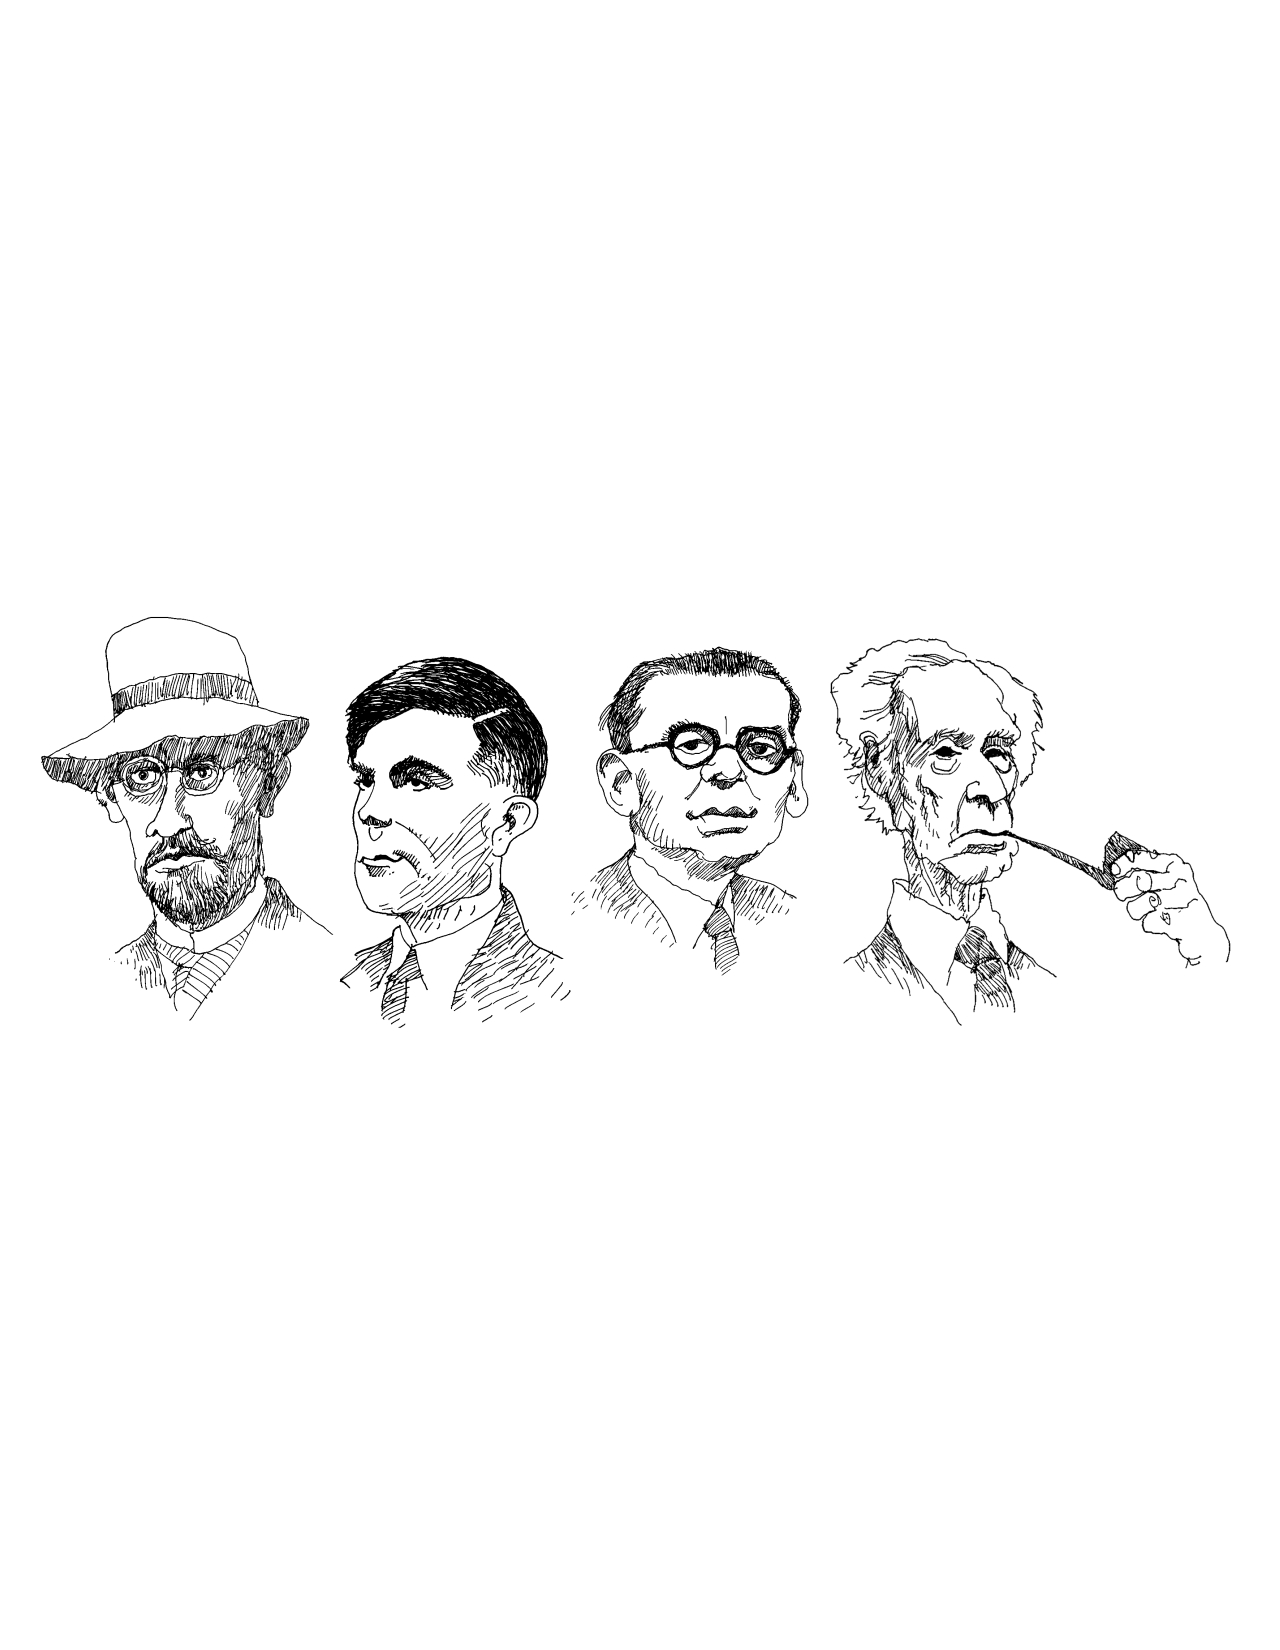
\includegraphics[scale=0.65]{figures/cover.jpeg}}} 
    \vspace*{5cm}
\endgroup
	%----------------------------------------------------------------------------------------
%	Páginas de Copyright
%----------------------------------------------------------------------------------------
\newpage
\noindent Valdigleis S. Costa

\noindent Professor Adjunto, Colegiado de Ciência da Computação

\noindent Universidade Federal do Vale do São Francisco

\noindent Salgueiro, PE\\

\noindent Copyright \copyright\ 2019-{\the\year} Valdigleis S Costa

\noindent Este texto  \textsc{NÃO}  possui qualquer tipo de vínculo editorial.

\noindent Página pessoal do autor \url{https://profvaldi.site}

\noindent As imagens usadas na capa pode ser encontradas no ótimo \textit{paper} de Chaitin \cite{chaitin2002figures}.

~\vfill

% Zera as configurações de formatação
\thispagestyle{empty}


\begin{figure*}[h]
	\centering
	
\includegraphics[width=0.15\linewidth]{figures/license}
\end{figure*}
\noindent Este material é licenciado sob a Licença Atribuição-NãoComercial-CompartilhaIgual 3.0 Não Adaptada (CC BY-NC-SA 3.0).  Você pode obter uma copia da licença acessando a página: 
\begin{center}
	\url{https://creativecommons.org/licenses/by-nc-sa/3.0/deed.pt_BR}
\end{center}
\noindent ou enviando uma carta para Creative Commons, 444 Castro Street, Suite 900, Mountain View, California, 94041, USA.

~\vfill

% Zera as configurações de formatação
\thispagestyle{empty}

\hrule
\vspace*{1cm}
%\noindent As imagens dos personagens Snuffles, Rick e Morty são encontradas facilmente pelo Google, o direito comercial sobre elas pertence totalmente aos seus criadores.\\

\noindent Este manuscrito é redigido usando um \textit{template} desenvolvido pelo próprio autor. Este texto foi escrito com {\LaTeX} e {\LaTeXe} nos ambientes de trabalho Debian/Ubuntu e Mac OS usando o \textit{software} TeXstudio e as distribuições  {\TeX}Live e Mac{\TeX}. \\ 

\noindent \textit{Release, \today--\currenttime} %
\newpage
	%----------------------------------------------------------------------------------------
%	Página de Disclaimer
%----------------------------------------------------------------------------------------
\begingroup
\thispagestyle{empty}
\begin{center}
	{\normalfont\fontsize{20}{20}\sffamily\selectfont \textbf{\textit{Disclaimer}}}\par
\end{center}

\vspace{1cm}

Este manuscrito está sendo construído tendo como base diversas notas de aula que eu preparei para cursos de:

\begin{multicols}{2}
	\begin{fieldsList}
		\item Matemática Discreta
		\item Lógica para Ciência da Computação
		\item Linguagens Formais e Autômatos
		\item Análise de Algoritmos
		\item Computabilidade
		\item Teoria dos Números para Computação
	\end{fieldsList}
\end{multicols}	

Uma vez que este manuscrito ainda é um projeto em andamento e possivelmente sua escrita nunca será realmente concluída com total aprovação de seu autor, é claro que você poderá encontrar diversos erros, que com toda certeza você leitor irá me enviar e-mails\footnote{E-mail do autor: \url{valdigleis.costa@univasf.edu.br}} ou \textit{issues}\footnote{Páginas de \textit{issues}: \url{https://github.com/valdigleis/Manuscrito/issues}} com reports de tais erros.

%Com respeito a organização do manuscrito é interessante ressaltar que ele não tem uma ordem geral para a leitura de capítulos, de fato, existem diversas ordem de leituras. Assim o autor recomenda a leitura na ordem com que o leitor for necessitando dos conteúdos, isto é, realizando \textbf{pulos}, \textbf{adiamentos} e \textbf{retomadas} de leitura entre os capítulos e seções.

%Além das básicas estruturas de definições, teoremas, lemas, exercícios, exemplos e etc, este manuscrito ainda conta com três tipos ``novos'' de ambientes sendo: as explicações Snuffles, observações do Rick e perguntas do Morty.

%\begin{SnufflesInfo}
%	O Snuffles é um cachorrinho que ficou super inteligente,  ele gosta de se gabar dando explicações ao leitor sobre temas do manuscrito.
%\end{SnufflesInfo}

%\begin{RickInfo}
%	O Rick como é um grande cientista conhece muito de tudo então durante o texto ele vai dando ao leitor observações de diversos tipos sobre os temas e mostrando outras formas de entender o mesmo assunto.
%\end{RickInfo}

%\begin{MortyInfo}
%	O Morty ainda é um adolescente que está crescendo e aprendendo, assim ele faz diversas perguntas a você leitor, já que o Rick está bêbado demais para responder e o Snuffles prefere fazer planos (para a revolução canina) do que explicar coisas ao Morty. Se você estiver com a mesma dúvida do Morty, pergunte ao seu professor em sala de aula, assim você sana a dúvida sua e do Morty.
%\end{MortyInfo}

\endgroup
\newpage
	%----------------------------------------------------------------------------------------
%	Página de Disclaimer
%----------------------------------------------------------------------------------------
\begingroup
\thispagestyle{empty}

\vspace*{\fill}
\centering
\noindent
\textit{Este trabalho é dedicado aos meus professores e alunos, vocês são um conjunto enumerável de bons motivos para continuar escrevendo!} 
\vspace*{\fill}

\endgroup
\newpage
	%----------------------------------------------------------------------------------------
%	Páginas de Agradecimentos
%----------------------------------------------------------------------------------------
\begingroup
\thispagestyle{empty}
\begin{center}
	{\normalfont\fontsize{20}{20}\sffamily\selectfont \textbf{Agradecimentos}}\par
\end{center}

\vspace{1cm}

Este manuscrito está sendo construído aos poucos e diversas pessoas com o tempo irão contribuir direta ou indiretamente para que ele fique cada vez melhor, assim dedico esta(s) página(s) a agradecer nominalmente a qualquer um que tenha ajudado:

\begin{itemize}
	\item {\color{red}Raul da Silva Martins} ({\color{blue} Discente univasf/2021}) - Apontou correções de conteúdo no texto.
	\item {\color{red}Matheus Barros Rosa} ({\color{blue} Discente univasf/2022}) - Apontou correções ortográficas no texto.
	\item {\color{red}Gabriel Ferreira Rodrigues} ({\color{blue} Discente univasf/2022}) - Apresentou problemas de nomenclatura em uma definição.
\end{itemize}

\endgroup
	%----------------------------------------------------------------------------------------
%	Página da Epigrafe
%----------------------------------------------------------------------------------------
\newpage
\pagestyle{empty} % Disable headers and footers for the following pages

\vspace*{\fill}
\epigraph{``Ciência da Computação está tão relacionada aos computadores quanto a Astronomia aos telescópios, Biologia aos microscópios, ou Química aos tubos de ensaio...''}{Edsger Wybe Dijkstra (1930-2002)}
	
\pagestyle{fancy} % Enable headers and footers again
	\pagestyle{empty} % Disable headers and footers for the following pages

\tableofcontents % Print the table of contents itself

\cleardoublepage % Forces the first chapter to start on an odd page so it's on the right side of the book

\pagestyle{fancy} % Enable headers and footers again
	
	%---------------------------------------------------------------------------------------
	%	Adicionando os elementos do texto
	%---------------------------------------------------------------------------------------
	\part{Ferramentas e Linguagem Básica}\label{Parte:basica}
	\chapter{Conjuntos}\label{cap:Conjuntos}

\epigraph{``-Comece pelo começo'', disse o Rei de maneira severa,\\ ``-E continue até chegar ao fim, então pare!''}{Lewis Carroll, Alice no País das Maravilhas.}

\section{Conjuntos e Elementos}\label{sec:ConjuntoElemento}

A ideia de conjunto é provavelmente o conceito mais fundamental compartilhado pelos mais diversos ramos da matemática. O primeiro grande estudioso que apresentou uma forma relativamente precisa para o conceito de conjunto foi o matemático alemão George Cantor (1845-1918) em seu seminal trabalho \cite{cantor1895}. A seguir será apresentada uma tradução não literal da definição original de Cantor.

\begin{definition}[Cantor]\label{def:ConjuntoCantor}
	Um \textbf{conjunto} $A$ é uma \textbf{coleção} numa totalidade $M$ de certos \textbf{objetos} distintos e bem-definidos $n$ que fazem parte da nossa percepção ou pensamento, tais objetos são chamados de \textbf{elementos} de $A$.
\end{definition}

Note que a definição apresentada por Cantor exige dois aspectos sobre a natureza dos elementos em um conjunto: (1) que eles sejam distintos entre si, ou seja, em um conjunto não poderá haver repetição de elementos e (2) os elementos devem ser bem-definidos. 

A definição de Cantor permite que sejam criados conjuntos com qualquer coisa que o indivíduo racional possa pensar ou perceber pelos seus sentidos. Agora, entretanto, deve-se questionar o que significa dizer que algo é bem-definido? Uma resposta satisfatória para essa perguntar é dizer que algo é bem-definido se esse algo pode ser descrito sem ambiguidades. 

É claro que qualquer coisa pode ser descrita a partir de suas propriedades, características ou atributos, sendo que essas propriedades sempre podem ser verificadas pelos sentidos no caso de objetos físicos, e sempre pode-se pensar e argumentar sobre elas no caso de objetos abstratos. Assim pode-se modificar um pouco a definição de Cantor para a definição que se segue.

\begin{definition}[Definição de Cantor Modificada]\label{def:ConjuntoMinha}
	Um \textbf{conjunto} $A$ é uma \textbf{coleção} numa totalidade $M$ de certos \textbf{objetos} $n$ distintos e que satisfazem certas propriedades, tais objetos são chamados de \textbf{elementos} de $A$.
\end{definition}

\begin{remark}
	A partir desse ponto será usado a nomenclatura discurso em vez de totalidade na especificação de conjuntos.
\end{remark}

Note que a Definição \ref{def:ConjuntoMinha} permite concluir que um conjunto pode ser visto como o agrupamento de entidades (os elementos) que satisfazem certas propriedades, ou ainda que, as propriedades definem os conjuntos. Prosseguindo nesse texto serão apresentadas as convenções da \textbf{teoria ingênua dos conjuntos} de forma usual, mas também serão apresentados os aspectos sintáticos e semânticos da teoria.

\begin{definition}[Notações Básicas]\label{def:NotacaoConjuntos1}
	As letras maiúsculas do alfabeto latino $A, B, \cdots, M,$ $N, \cdots, Z$ como e sem indexação serão usadas como variáveis para representar conjuntos e as letras minúsculas $a, b, \cdots, m, n, \cdots, z$ como e sem indexação serão usadas como meta-variáveis para representar elementos.
\end{definition}

Assim a sintaxe da teoria ingênua dos conjuntos diz que letras minúsculas sempre representam elementos e letras maiúsculas sempre representam os conjuntos.

\begin{remark}
	O termo variável é usado para designar símbolos (ou palavras) de uma linguagem responsáveis por representar de forma genérica as entidades da teoria que a linguagem descreve (para detalhes leia \cite{sato2003}), ou seja,  são ``apelidos'' ou ``rótulos'' para as entidades.
\end{remark}

Como dito anteriormente uma propriedade $\textbf{P}$ é responsável por definir um conjunto, pois todos os elementos no conjunto devem satisfazer (ou possuir) tal propriedade. Tendo isso em mente pode-se introduzir a definição a seguir.

\begin{definition}[Notação compactada]\label{def:NotacaoCompacta}
	Um conjunto $A$ definido por alguma propriedade $\textbf{P}$ é representada na \textbf{forma compacta} como:
	\begin{equation}
		A = \{ x \mid \textbf{P}\}
	\end{equation}
\end{definition}

Na notação compacta $A = \{ x \mid \textbf{P}\}$ o símbolo $A$ é chamado de rótulo do conjunto, e a parte $\{ x \mid \textbf{P}\}$ será chamada neste manuscrito de forma estrutural do conjunto.

\begin{remark}
	A notação compacta $A = \{ x \mid \textbf{P}\}$ é na verdade uma palavra da linguagem da teoria ingênua dos conjuntos, a semântica de tal palavra pode ser interpretada como: ``$A$ é o conjunto de todos os $x$'s que satisfazem (ou possuem) a propriedade $\textbf{P}$.
\end{remark}

\begin{example}\label{exe:conjuntos}
	Os seguintes conjuntos estão bem representados na notação compacta.
	\begin{itemize}
		\item[(a)] $X = \{a \mid a \mbox{ é uma cidade do Brasil}\}$.
		\item[(b)] $K = \{m \mid m \mbox{ é um animal mamífero}\}$.
		\item[(c)] $L = \{x \mid 0 \leq x < 10 \mbox{ e } x \mbox{ é um número impar}\}$.
		\item[(d)] $C = \{b \mid b \mbox{ é uma vogal}\}$.
	\end{itemize}
\end{example}

Para continuar o desenvolvendo da linguagem da teoria dos conjuntos, é conveniente relembrar ao leitor os símbolos usados como rótulos para representar os conjuntos numéricos mais importantes da matemática.

\begin{definition}[Símbolos dos conjuntos numéricos]\label{def:SimbolosConjuntos}
	O conjunto dos números naturais\footnote{Neste manuscrito é considerado que o conjuntos dos naturais corresponde ao conjunto $\{0, 1, 2, \cdots\}$.}, inteiros, racionais, irracionais, reais e complexos são representados respectivamente por   $\mathbb{N}$, $\mathbb{Z}$,  $\mathbb{Q}$,  $\mathbb{I}$,  $\mathbb{R}$ e  $\mathbb{C}$.
\end{definition}

\begin{remark}
	Neste manuscrito $\mathbb{N}_*, \mathbb{Z}_*, \mathbb{Q}_*$ e $\mathbb{R}_*$ irão denotar receptivamente o conjunto dos naturais, inteiros, racionais e reais sem o $0$. Já $\mathbb{Z}^+, \mathbb{Q}^+$ e $\mathbb{R}^+$ irão denotar receptivamente o conjunto dos inteiros, racionais e reais positivos. E por fim, $\mathbb{Z}^-, \mathbb{Q}^-$ e $\mathbb{R}^-$ irão denotar receptivamente o conjunto dos inteiros, racionais e reais negativos.
\end{remark}

Seguindo com o desenvolvimento da teoria dos conjuntos a definição a seguir estabelece um relacionamento (ou relação) de pertinência entre os conjuntos e os elementos do discurso.

\begin{definition}[Pertinência]\label{def:Pertinencia}
	Seja $A$ um conjunto definido sobre um discurso $M$ por uma propriedade $\textbf{P}$ e seja $x$ um elemento do discurso. Se o elemento $x$ possui (ou satisfaz) a propriedade $\textbf{P}$, então é dito que $x$ pertence a $A$, denotado por $x \in A$. Caso $x$ não possui (ou satisfaça) a propriedade $\textbf{P}$, então é dito que $x$ não pertence a $A$, denotado por $x \notin A$
\end{definition}

A Definição \ref{def:Pertinencia} está introduzindo novas entidades da linguagem da teoria dos conjuntos, sento tais objetos as palavras da forma $\underline{\ \ \ } \in \underline{\ \ \ }$ e da forma $\underline{\ \ \ } \notin \underline{\ \ \ }$. Em tais palavras o símbolo do lado esquerdo de $\in$ e $\notin$ sempre será visto como sendo um elemento do discurso ou uma variável que representa tal elemento, por outro lado, o símbolo do lado direito de $\in$ e $\notin$ sempre devem ser o rótulo ou a forma estrutural de um conjunto.

\begin{remark}
	Quando $x \in A$, em alguns texto como em \cite{lipschutz1978-TC} é comum o uso das interpretações semânticas: ``$A$ possui $x$'' ou que ``$x$ faz parte de $A$'', durante este manuscrito possa ser que uma dessas (ou ambas) interpretações sejam usadas, além da semântica padrão: $x \mbox{ pertence a }  A$.
\end{remark}

\begin{example}
	Seja $A$ o conjunto definido sobre a propriedade ``é professor de Ciência da Computação na univasf'' tem-se que o professor $\mbox{Rodrigo} \in A$. Já para os professores Regivan e Benjamin tem-se que $\mbox{Regivan, Benjamin} \notin A$. 
\end{example}

\begin{example}
	Seja $A_1$ o conjunto definido pela propriedade ``Clubes da primeira divisão do campeonato brasileira de futebol do ano 2021'' tem-se então que $\mbox{Vasco} \notin A_1$.
\end{example}

Há casos entretanto, que a notação compacta é descartada e assim os conjuntos podem ser escritos simplesmente listando seus elementos entre as chaves da forma estrutural, isso em geral acontece quando o conjunto é finito\footnote{Por hora o leitor deve considerar que um conjunto finito é aquele que o leitor poderia contar o número de elementos, em capítulos futuros serão formalizados os conceitos de conjuntos finitos e infinitos.} e possui um número não muito grande de elementos.

\begin{example}
	A seguir são listados alguns conjuntos finitos escritos descartando a notação compacta.
	\begin{itemize}
		\item[(a)] O conjunto das vogais pode ser representado como $A = \{a,e,i,o,u\}$.
		\item[(b)] O conjunto das siglas dos estados nordestinos pode ser escrito como $E = \{RN, PE,$ $PB, MA, CE, SE,$ $AL, BA, PI\}$.
		\item[(c)] O conjunto dos naturais menores que 10 é escrito como $N_{10} = \{0, 1, 2, 3, 4, 5, 6, 7, 8, 9\}$.
	\end{itemize}
\end{example}

\begin{remark}
	Quando se optar por escrever um conjunto finito apenas listando os seus elementos entre chaves a ordem com que os elementos aparecem não importa, assim tem-se que os conjuntos $\{a, e, i, o , u\}$ e $\{e, u, i, a, o\}$ são na verdade o mesmo conjunto.
\end{remark}

Note que a relação de pertinência  apresentada anteriormente (Definição \ref{def:Pertinencia}) relaciona elementos e conjuntos, existe também uma relação extremamente fundamental dentro da teoria dos conjuntos que é definida entre dois conjuntos. 

A relação entre conjuntos recebe o nome de \textbf{relação de inclusão}, entretanto, como dito em \cite{lipschutz1978-TC}, é comum que quando um conjunto $A$ estiver relacionado com um conjunto $B$ pela relação de inclusão, se usar a interpretação semântica ``$A$ é subconjunto de $B$'', em vez de, ``$A$ está incluso em $B$''. A seguir é apresentado formalmente esta relação.

\begin{definition}[Relação de inclusão]\label{def:RelacaoInclusao}
	Dado dois conjuntos $A$ e $B$ quaisquer, é dito que $A$ é subconjunto de $B$, denotado por $A \subseteq B$, quando todo $x \in A$ é tal que $x \in B$.
\end{definition}

\begin{example}\label{exe:ConjuntoHerdeiro}
	Dado o conjunto $\mathbb{Z}$ tem-se que o conjunto $N = \{x \mid x \in \mathbb{Z} \mbox{ e } x = 2k \mbox{ para algum } k \in \mathbb{Z}\}$ é claramente um subconjunto de $\mathbb{Z}$ pois todo número par é também um número inteiro.
\end{example}

\begin{example}\label{exe:Inclusao}
	As seguintes relações de inclusão se verificam:
	\begin{itemize}
		\item[(a)] $\{a, e, u\} \subseteq \{a, e, o, i , u\}$.
		\item[(b)] $\{x \mid x \mbox{ é uma cidade do PE}\} \subseteq \{x \mid x \mbox{ é uma cidade do Brasil}\}$.
		\item[(c)] $\{x \mid x = 2k \mbox{ para algum } k \in \mathbb{N}\} \subseteq \mathbb{N}$.
		\item[(d)] $\{\mbox{Brasil}\} \subseteq \{x \mid x \mbox{ é um país do continente americano}\}$
	\end{itemize}
\end{example}

É obvio que a Definição \ref{def:RelacaoInclusao} está introduzindo novas entidades da linguagem da teoria dos conjuntos, sento tais objetos as palavras da forma $\underline{\ \ \ } \subseteq \underline{\ \ \ }$. Em tais palavras os elementos à esquerda e à direita do símbolo $\subseteq$ sempre devem ser o rótulos ou as formas estruturais de conjuntos. Em oposição a relação de inclusão existe a relação de não inclusão descrita a seguir.

\begin{definition}[Relação de inclusão]\label{def:RelacaoNaoInclusao}
	Dado dois conjuntos $A$ e $B$ quaisquer, é dito que $A$ é não subconjunto de $B$, denotado por $A \not\subseteq B$, quando existe pelo menos um $x \in A$ tal que $x \not\in B$.
\end{definition}

\begin{example}\label{exe:NaoInclusao}
	Seja $A = \{-1, 0, 1\}$ tem-se que $A \not\subseteq \mathbb{N}$.
\end{example}

Existe também a possibilidade de todos os elementos de $A$ serem elementos de $B$, mas que $B$ possua outros elementos que não fazem parte de $A$, nesse caso é dito que $A$ é um \textbf{subconjunto próprio} de $B$, e isto é denotado como $A \subset B$. 

\begin{example}\label{exe:InclusaoPropria}
	As seguintes relações de inclusão se verificam:
	\begin{itemize}
		\item[(a)] $\{1, 2\} \subset \mathbb{R}$.
		\item[(b)] $\{x \mid x \mbox{ é uma cidade do PE}\} \subset \{x \mid x \mbox{ é uma cidade do Brasil}\}$.
		\item[(c)] $\mathbb{Z}_+ \subset \mathbb{Z}$.
	\end{itemize}
\end{example}

\begin{remark}
	Note que todo subconjunto $A$ de um conjunto $B$ pode ser visto como um conjunto construído sobre os elementos de $B$ que satisfazem uma certa propriedade $\textbf{P}$, isto é, tem-se que todo subconjunto $A$ é um conjunto da seguinte forma:
	$$A = \{x \mid x \in B \mbox{ e } x \mbox{ satisfaz } \textbf{P}\}$$
	também é possível encontrar a notação $A = \{x \in B  \mid x \mbox{ satisfaz } \textbf{P}\}$, sempre que possível esse manuscrito irá adotar a segunda notação.
\end{remark}

Usando a ideia de subconjunto pode-se como apresentado na literatura em obras como \cite{abe1991-TC, halmos2001, lipschutz1978-TC} introduzir a ideia de igualdade entre conjuntos, esta noção é apresentada formalmente como se segue.

\begin{definition}[Igualdade de conjuntos]\label{def:IgualdadeConjuntos}
	\cite{abe1991-TC} Dois conjuntos $A$ e $B$ são iguais, denotado por $A = B$, se e somente se, $A \subseteq B$ e $B \subseteq A$.
\end{definition}

\begin{theorem}[Teorema da igualdade]
	Sejam $A, B$ e $C$ conjuntos quaisquer. Então:
	\begin{enumerate}
		\item $A = A$.
		\item Se $A = B$, então $B = A$.
		\item Se $A = B$ e $B = C$, então $A = C$.
	\end{enumerate}
\end{theorem}

Dentro da teoria dos conjuntos alguns conjuntos possuem tanta importância e destaque que eles recebem nomes e símbolos próprios. 

\begin{definition}[Conjunto Universo]\label{def:ConjuntoUniverso}
	O conjunto universo, ou universo do discurso, denotado por $\mathbb{U}$, é um conjunto que possui todos os elementos sobre os quais se ``fala\footnote{O termo fala aqui diz respeito ao ato pensar ou argumentar sobre os objetos.}''.
\end{definition}

O universo do discurso não é único, de fato o mesmo muda em função sobre o que se está ``discursando'', por exemplo, pode-se pensar em um universo do discurso para falar sobre números, carros, pessoas, animais, palavras, times de futebol e etc.

\begin{definition}[Conjunto vazio]\label{def:ConjuntoVazio}
	O conjunto vazio, denotado por $\emptyset$, corresponde a um conjunto que não possui nenhum elemento.
\end{definition} 

Uma propriedade interessante sobre o conjunto vazio é apresentada a seguir, tal propriedade garante que o conjunto vazio está presente em qualquer outro conjunto existente.

\begin{theorem}\label{teo:ConjuntoVazioSubDeTodos}
	Para todo conjunto $A$ tem-se que $\emptyset \subseteq A$.
\end{theorem}

\begin{proof}
	Suponha por absurdo que existe um conjunto $A$ tal que $\emptyset \not\subseteq A$, assim por definição  existe pelo menos um $x \in \emptyset$ tal que $x \notin A$, mas isto é um absurdo já que o vazio não possui elementos, e portanto, a afirmação que $\emptyset \not\subseteq A$ é falsa, logo, $\emptyset \subseteq A$ é verdadeiro para qualquer que seja o $A$.
\end{proof}

\begin{note}
	Neste manuscrito ao final das demonstrações será sempre colocado o símbolo $\blacksquare$, tal símbolo é conhecido como túmulo de Halmos\footnote{Em inglês esse símbolo é conhecido como \textit{tombstone}, e tal símbolo foi usado para marcar o final de uma demonstração inicialmente pelo matemático Paul Halmos (1916-2006).}, este símbolo será usado para substituir a notação q.e.d. (``\textit{quod erat demonstrandum}'') usando por outras fontes bibliográficas para marcar o ponto de finalização de uma demonstração. 
\end{note}

Agora que foram apresentados os conjuntos universo e vazio, é conveniente comentar sobre uma situação específica da teoria dos conjuntos como apresentada até aqui. Pelo que foi apresentado até agora já se sabe que os itens em um conjunto são chamados de elementos, entretanto, não existe qualquer restrição, além de ser bem definido, para a natureza (ou tipo) dos elementos em um conjunto. Isso possibilita que seja possível definir por exemplo um conjunto de conjuntos, isto é, um conjunto em que os elementos são também conjuntos.

\begin{definition}[Família de Conjuntos]\label{def:Familia}
	Um conjunto $A$ cujo os elementos são todos conjuntos, isto é, um conjunto da forma $A = \{x \mid x \mbox{ é um conjunto}\}$, é chamado de \textbf{família de conjuntos}.
\end{definition}

\begin{example}\label{exe:Familia}
	Os conjuntos: 
	$$A_1 = \{\mathbb{Z}^*_+, \mathbb{Z}_-, \{\pi, \sqrt{-1}\}\} \mbox{ e } A_2 = \{\{a, b\}, \{\clubsuit, \spadesuit, \heartsuit, \lozenge\}, \mathbb{R}\}$$
	são ambos famílias.
\end{example}

\begin{remark}
	Além do termo família algumas obras como \cite{lipschutz1978-TC} também usam a nomenclatura classe, neste manuscrito só será usado o termo classe em situações bem específicas como por exemplo, as classes de equivalência em um espaço quociente.
\end{remark}

\section{Operações sobre conjuntos}\label{sec:OperacoesConjuntos}

Seguindo a mesma organização de conteúdo apresentada em \cite{lipschutz2013-MD}, pode-se agora introduzir uma série de operações conjuntistas, isto é, operações que agem diretamente sobre conjuntos de ``entrada'' produzindo como ``saída'' novos conjuntos.

\begin{definition}[União de conjuntos]\label{def:UniaoConjuntos}
	Sejam $A$ e $B$ dois conjuntos quaisquer, a união de $A$ com $B$, denotada por $A \cup B$, corresponde ao seguinte conjunto.
	$$A \cup B = \{x \mid x \in A \mbox{ ou } x \in B\}$$
\end{definition}

\begin{example}\label{exe:UniaoDeConjuntos1}
	Dados os dois conjuntos $A = \{x \in \mathbb{N} \mid x = 2i \mbox{ para algum } i \in \mathbb{N}\}$ e $B = \{x \in \mathbb{N} \mid x = 2j + 1 \mbox{ para algum } j \in \mathbb{N}\}$ tem-se que $A \cup B = \mathbb{N}$.
\end{example}

\begin{example}\label{exe:UniaoDeConjuntos2}
	Seja $N = \{1, 2, 3, 6\}$ e $L = \{4, 6\}$ tem-se que $N \cup L = \{1, 4, 6, 3, 2\}$.
\end{example}

Como apontado em \cite{lipschutz1978-TC} alguns livros usam a notação $A + B$ para representar a união, é comum nesse caso não usar a nomenclatura união, em vez disso, é usado o termo soma de conjunto, entretanto, trata-se da mesma operação de união apresentada na definição anterior.

\begin{definition}[Interseção de conjuntos]\label{def:IntersecaoConjuntos}
	Sejam $A$ e $B$ dois conjuntos quaisquer, a interseção de $A$ com $B$, denotada por $A \cap B$, corresponde ao seguinte conjunto.
	$$A \cap B = \{x \mid x \in A \mbox{ e } x \in B\}$$
\end{definition}

\begin{example}\label{exe:IntersecaoDeConuuntos1}
	Dado $A_1 = \{x \in \mathbb{N} \mid x \mbox{ é múltiplo de } 2\}$ e $A_2 = \{x \in \mathbb{N} \mid x \mbox{ é múltiplo de } 3\}$ tem-se que $A_1 \cap A_2 = \{x \in \mathbb{N} \mid x \mbox{ é múltiplo de } 6\}$.
\end{example}

\begin{example}\label{exe:IntersecaoDeConuuntos2}
	Seja $A = \{1, 2, 3\}, B = \{2, 3, 4, 5\}$ e $C = \{5\}$ tem-se que:
	\begin{itemize}
		\item[(a)] $A \cap B = \{2, 3\}$.
		\item[(b)] $A \cap C = \emptyset$.
		\item[(c)] $B \cap C = \{5\}$.
		\item[(d)] $B \cap B = \{2, 3, 4, 5\} = B$.
	\end{itemize}
\end{example}

Com respeito as propriedades equacionais das operações de união e interseção tem-se como exposto em \cite{lipschutz2013-MD} os seguintes resultados para todo $A, B$ e $C$.

\begin{table}[h]
	\centering
	%\scriptsize
	\begin{tabular}{cccc}
		\hline
		identificador & None & União & Interseção  \\
		\hline
		$p_1$ & Idempotência &  $A \cup A = A$ & $A \cap A = A$  \\
		$p_2$ & Comutatividade & $A \cup B = B \cup A$ & $A \cap B = B \cap A$ \\
		$p_3$ & Associatividade & $A \cup (B \cup C) = (A \cup B) \cup C$ & $A \cap (B \cap C) = (A \cap B) \cap C$ \\
		$p_4$ & Distributividade & $A \cup (B \cap C) = (A \cup B) \cap (A \cup C)$ & $A \cap (B \cup C) = (A \cap B) \cup (A \cap C)$\\
		$p_5$ & Neutralidade &  $A \cup \emptyset = A$ & $A \cap \mathbb{U} = A$ \\
		$p_6$ & Absorção & $A \cup \mathbb{U} = \mathbb{U}$ & $A \cap \emptyset = \emptyset$ \\
		\hline
	\end{tabular}
	\caption{Tabela das propriedades das operações de união e interseção.}
	\label{tab:PropriedadesUniaoIntersecao}
\end{table}

Além das propriedades apresentadas pela Tabela \ref{tab:PropriedadesUniaoIntersecao}, a união e a interseção possuem propriedades ligadas a relação de inclusão.

\begin{theorem}\label{teo:MonotonicidadeDaUniaoIntersecao}
	Para quaisquer conjuntos $A$ e $B$ tem-se que:
	\begin{itemize}
		\item[i.] $A \subseteq (A \cup B)$.
		\item[ii.] $(A \cap B) \subseteq A$
	\end{itemize}
\end{theorem}

\begin{proof}
	Direta das Definições \ref{def:RelacaoInclusao}, \ref{def:UniaoConjuntos} e \ref{def:IntersecaoConjuntos}.
\end{proof}

A partir da definição de interseção é estabelecido um conceito de extrema valia para a teoria dos conjuntos e suas aplicações, tal conceito é o estado de disjunção entre dois conjuntos.

\begin{definition}[Conjuntos disjuntos]\label{def:ConjuntosDisjuntos}
	Dois conjuntos $A$ e $B$ são ditos disjuntos sempre que $A \cap B = \emptyset$.
\end{definition}

\begin{example}\label{exe:ConjuntosDisjuntos}
	Seja $A = \{1, 2, 3\}, B = \{2, 3, 5\}$ e $C = \{5\}$ tem-se que $A$ e $C$ são disjuntos, por outro lado, $A$ e $B$ não são disjuntos entre si, além disso, $B$ e $C$ também não são disjuntos entre si.
\end{example}

\begin{definition}[Complemento de conjuntos]\label{def:ComplementoConjuntos}
	Seja $A \subseteq \mathbb{U}$ para algum universo $\mathbb{U}$, o complemento de $A$, denotado por $\overline{A}$, corresponde ao seguinte conjunto:
	$$\overline{A} = \{x \in \mathbb{U} \mid x \notin A\}$$
\end{definition}

\begin{example}\label{exe:Complemento}
	Dado $P = \{ x \in \mathbb{Z} \mid x = 2k \mbox{ para algum } k \in \mathbb{Z}\}$ tem-se então o seguinte complemento $\overline{P} = \{ x \in \mathbb{Z} \mid x = 2k + 1 \mbox{ para algum } k \in \mathbb{Z}\}$.
\end{example}

\begin{example}
	Dado um universo do discurso $\mathbb{U}$ tem-se direto da definição que $\overline{\mathbb{U}} = \emptyset$, e obviamente, $\overline{\emptyset} = \mathbb{U}$.
\end{example}

\begin{theorem}\label{teo:PropriedadesComplemento}
	Dado um conjunto $A$ tem-se que:
	\begin{itemize}
		\item[i.] $A \cup \overline{A} = \mathbb{U}$.
		\item[ii.] $A \cap \overline{A} = \emptyset$.
		\item[iii.] $\overline{\overline{A}} = A$.
	\end{itemize}
\end{theorem}

\begin{proof}
	Direta das Definições \ref{def:UniaoConjuntos}, \ref{def:IntersecaoConjuntos} e \ref{def:ComplementoConjuntos}.
\end{proof}

\begin{remark}
	A propriedade $(iii)$ apresentada no Teorema \ref{teo:PropriedadesComplemento} costuma ser chamada involução, como dito em \cite{lipschutz1978-TC}.
\end{remark}

Além das propriedades apresentadas no Teorema \ref{teo:PropriedadesComplemento} o complemento também apresenta propriedades ligadas diretamente a união e a interseção, tais propriedades são uma versão conjuntistas das famosas leis De Morgan (ver \cite{carmo2013, joaoPavao2014, lipschutz2013-MD}) muito conhecidas pelos estudiosos da área de lógica, a seguir são apresentadas as leis De Morgan para a linguagem teoria dos conjuntos.

\begin{table*}[h]
	\centering
	\begin{tabular}{lc}
		\textbf{(DM1) Lei De Morgan 1ª forma:} & $\overline{(A \cup B)} = \overline{A} \cap \overline{B}$\\
		\textbf{(DM2) Lei De Morgan 2ª forma:} & $\overline{(A \cap B)} = \overline{A} \cup \overline{B}$\\
	\end{tabular}
\end{table*}

Seguindo com este manuscrito, uma outra importante operação sobre conjuntos é a diferença entre conjuntos. A diferença entre conjunto apresenta duas formas, a primeira considerada por muito com a diferença natural \cite{carmo2013} e existe também a diferença simétrica, que em um certo sentido, pode ser usada para medir a  dissimetria entre conjuntos, ambas as operações são definidas formalmente a seguir.

\begin{definition}[Diferença de conjuntos]\label{def:DiferencaConjuntos}
	Dado dois conjuntos $A$ e $B$, a diferença de $A$ e $B$, denotado por $A - B$ corresponde ao seguinte conjunto:
	$$A - B = \{x \in A \mid x \notin B\}$$
\end{definition}

\begin{example}\label{exe:DiferencaConjuntos1}
	Dado os conjuntos $S = \{a, b, c, d\}$ e $T = \{f, b, g, d\}$ tem-se os seguintes conjuntos de diferença: $S - T = \{a, c\}$ e $T - S = \{f, g\}$.
\end{example}

\begin{example}\label{exe:DiferencaConjuntos2}
	Dado so conjuntos $\mathbb{Z}$ e $\mathbb{Z}_+^*$ tem-se que $\mathbb{Z} - \mathbb{Z}_+^* = \mathbb{Z}_-$.
\end{example}

\begin{remark}
	Note que o Exemplo \ref{exe:DiferencaConjuntos1} mostra que a operação de diferença de conjuntos não é comutativa.
\end{remark}

\begin{theorem}\label{teo:BasicoDiferencaConjuntos}
	Para todo $A$ e $B$ tem-se que:
	\begin{itemize}
		\item[i.] $A - B = A \cap \overline{B}$.
		\item[ii.] Se $B \subset A$, então $A - B = \overline{B}$.
	\end{itemize}
\end{theorem}

\begin{proof}
	Dado os conjuntos $A$ e $B$ segue que:
	\begin{itemize}
		\item[i.] Por definição para todo $x \in A - B$ tem-se que $x \in A$ e $x \notin B$, mas isto só é possível se, e somente se, $x \in A$ e $x \in \overline{B}$, e por sua vez, isto só é possível se, e somente se, $x \in A \cap \overline{B}$, portanto, tem-se que $A - B = A \cap \overline{B}$.
		\item[ii.] Suponha que $B \subset A$, ou seja, todo $x \in B$ e tal que $x \in A$. Agora note que todo $x \in A - B$ é tal que $x \in A$ e $x \notin B$, e portanto, pela Definição \ref{def:DiferencaConjuntos} e pela hipótese de $B \subset A$ é claro que $A - B = \overline{B}$.
	\end{itemize}
\end{proof}

A seguir são apresentadas duas séries de igualdades notáveis relacionadas a diferença entre conjuntos.

\begin{theorem}\label{teo:ElementarDiferencaConjuntos1}
	Sejam $A$ e $B$ subconjuntos de um universo $\mathbb{U}$, tem-se que:
	\begin{itemize}
		\item[a.] $A - \emptyset = A$ e $\emptyset - A = \emptyset$.
		\item[b.] $A - \mathbb{U} = \emptyset$ e $\mathbb{U} - A = \overline{A}$.
		\item[c.] $A - A = \emptyset$.
		\item[d.] $A - \overline{A} = A$.
		\item[e.] $\overline{(A - B)} = \overline{A} \cup B$.
		\item[f.] $A - B = \overline{B} - \overline{A}$.
	\end{itemize}
\end{theorem}

\begin{proof}
	Para todas as equações a seguir suponha que $A$ e $B$ são subconjuntos de um universo $\mathbb{U}$ assim segue que:
	\begin{itemize}
		\item[a.] 
		\begin{eqnarray*}
			A - \emptyset & \stackrel{Teo. \  \ref{teo:BasicoDiferencaConjuntos}(i)}{=}& A \cap \overline{\emptyset} \\
			& = & A \cap \mathbb{U} \\
			& \stackrel{Tab. \ \ref{tab:PropriedadesUniaoIntersecao}(p_5)}{=} & A
		\end{eqnarray*}
		e também tem-se que, 
		\begin{eqnarray*}
			\emptyset - A &\stackrel{Teo. \  \ref{teo:BasicoDiferencaConjuntos}(i)}{=}& \emptyset \cap \overline{A}\\
			&\stackrel{Tab. \ \ref{tab:PropriedadesUniaoIntersecao}(p_6)}{=}& \emptyset
		\end{eqnarray*}
		
		\item[b.] A prova tem um raciocínio similar a demonstração do item anterior, assim será deixado como exercício ao leitor.
		\item[c.] Trivial pela própria Definição \ref{def:DiferencaConjuntos}.
		\item[d.] 
		\begin{eqnarray*}
			A - \overline{A} &\stackrel{Teo. \  \ref{teo:BasicoDiferencaConjuntos}(i)}{=}& A \cap \overline{\overline{A}}\\ 
			&\stackrel{Teo. \ \ref{teo:PropriedadesComplemento}(iii)}{=}& A \cap A\\
			&\stackrel{Tab. \ \ref{tab:PropriedadesUniaoIntersecao}(p_1)}{=}& A
		\end{eqnarray*} 
		\item[e.] 
		\begin{eqnarray*}
			\overline{(A - B)} &\stackrel{Teo. \  \ref{teo:BasicoDiferencaConjuntos}(i)}{=}& \overline{(A \cap \overline{B})}\\
			&\stackrel{\textbf{(DM2)}}{=}& \overline{A} \cup \overline{\overline{B}}\\
			&\stackrel{Teo. \ \ref{teo:PropriedadesComplemento}(iii)}{=}&  \overline{A} \cup  B
		\end{eqnarray*}
		\item[f.] 
		\begin{eqnarray*}
			A - B &\stackrel{Teo. \  \ref{teo:BasicoDiferencaConjuntos}(i)}{=}& A \cap \overline{B}\\
			&\stackrel{Tab. \ \ref{tab:PropriedadesUniaoIntersecao}(p_2)}{=}& \overline{B} \cap A\\
			&\stackrel{Teo. \ \ref{teo:PropriedadesComplemento}(iii)}{=}& \overline{B} \cap \overline{\overline{A}}\\
			&\stackrel{Teo. \  \ref{teo:BasicoDiferencaConjuntos}(i)}{=}&  \overline{B} - \overline{A}
		\end{eqnarray*}
	\end{itemize}
	E assim a prova está concluída.
\end{proof}

\begin{note}
	Na demonstração do Teorema \ref{teo:ElementarDiferencaConjuntos1} apresentada anteriormente, algumas vezes foi escrito o símbolo de $=$ com um texto acima, isso é uma técnica comum na escrita de demonstrações matemáticas, o entendimento que leitor precisa ter é que ao escrever $\stackrel{\kappa}{=}$ significa que a igualdade segue (ou é garantida) pela propriedade ou resultado $\kappa$. Durante este manuscrito em algumas demonstrações uma escrita similar irá aparecer para outros símbolos (implicações, bi-implicações e etc.) que serão introduzidos no decorrer deste manuscrito.
\end{note}

\begin{theorem}\label{teo:ElementarDiferencaConjuntos2}
	Sejam $A, B$ e $C$ subconjuntos de um universo $\mathbb{U}$, tem-se que:
	\begin{itemize}
		\item[a.] $(A - B) - C = A - (B \cup C)$.
		\item[b.] $A - (B - C) = (A - B) \cup (A \cap C)$.
		\item[c.] $A \cup (B - C) = (A \cup B) - (C - A)$.
		\item[d.] $A \cap (B - C) = (A \cap B) - (A \cap C)$.
		\item[e.] $A - (B \cup C) = (A - B) \cap (A - C)$.
		\item[f.] $A - (B \cap C) = (A - B) \cup (A - C)$.
		\item[g.] $(A \cup B) - C = (A - C) \cup (B - C)$.
		\item[h.] $(A \cap B) - C = (A - C) \cap (B - C)$.
		\item[i.] $A - (A - B) = A \cap B$.
		\item[j.] $(A - B) - B = A - B$.´
	\end{itemize}
\end{theorem}

\begin{proof}
	Para todas as equações a seguir suponha que $A, B$ e $C$ são subconjuntos de um universo $\mathbb{U}$ assim segue que:
	\begin{itemize}
		\item[a.] 
		\begin{eqnarray*}
			(A - B) - C & \stackrel{Teo. \  \ref{teo:BasicoDiferencaConjuntos}(i)}{=} & (A \cap \overline{B}) \cap \overline{C}\\
			& \stackrel{Tab. \ \ref{tab:PropriedadesUniaoIntersecao}(p_3)}{=} & A \cap (\overline{B} \cap \overline{C})\\
			& \stackrel{\textbf{(DM1)}}{=} & A \cap \overline{(B \cup C)}\\
			& \stackrel{Teo. \  \ref{teo:BasicoDiferencaConjuntos}(i)}{=} & A - (B \cup C)
		\end{eqnarray*}
		\item[b.]
		\begin{eqnarray*}
			A - (B - C) & \stackrel{Teo. \  \ref{teo:BasicoDiferencaConjuntos}(i)}{=} & A \cap \overline{(B - C)} \\
			& \stackrel{Teo. \ \ref{teo:ElementarDiferencaConjuntos1}(e)}{=} & A \cap (\overline{B} \cup C)\\
			& \stackrel{Tab. \ \ref{tab:PropriedadesUniaoIntersecao}(p_4)}{=} & (A \cap \overline{B}) \cup (A \cap C)\\
			& \stackrel{Teo. \  \ref{teo:BasicoDiferencaConjuntos}(i)}{=} & (A - B) \cup (A \cap C)
		\end{eqnarray*} 
		\item[c.] 
		\begin{eqnarray*}
			A \cup (B - C) & \stackrel{Teo. \  \ref{teo:BasicoDiferencaConjuntos}(i)}{=} & A \cup (B \cap \overline{C})\\
			& \stackrel{Tab. \ \ref{tab:PropriedadesUniaoIntersecao}(p_4)}{=} &  (A \cup B) \cap (A \cup \overline{C})\\
			& \stackrel{Tab. \ \ref{tab:PropriedadesUniaoIntersecao}(p_2)}{=} & (A \cup B) \cap (\overline{C} \cup A)\\
			& \stackrel{Teo. \ \ref{teo:PropriedadesComplemento}(iii)}{=}& (A \cup B) \cap (\overline{C} \cup \overline{\overline{A}})\\
			& \stackrel{\textbf{(DM2)}}{=}& (A \cup B) \cap \overline{(C \cap \overline{A})}\\
			& \stackrel{Teo. \  \ref{teo:BasicoDiferencaConjuntos}(i)}{=}& (A \cup B) - (C \cap \overline{A})\\
			& \stackrel{Teo. \  \ref{teo:BasicoDiferencaConjuntos}(i)}{=}& (A \cup B) - (C - A)\\
		\end{eqnarray*}
		\item[d.] 
		\begin{eqnarray*}
			A \cap (B - C) & \stackrel{Teo. \  \ref{teo:BasicoDiferencaConjuntos}(i)}{=}& A \cap (B \cap \overline{C})\\
			& = & \emptyset \cup ( A \cap (B \cap \overline{C}))\\
			& \stackrel{Tab. \ \ref{tab:PropriedadesUniaoIntersecao}(p_2)}{=} & \emptyset \cup ( (A \cap B) \cap \overline{C})\\
			& \stackrel{Tab. \ \ref{tab:PropriedadesUniaoIntersecao}(p_6)}{=} & (\emptyset \cap B) \cup ( (A \cap B) \cap \overline{C})\\
			& \stackrel{Teo. \ \ref{teo:PropriedadesComplemento}(ii)}{=} & ((A \cap \overline{A}) \cap B) \cup ( (A \cap B) \cap \overline{C})\\
			& \stackrel{Tab. \ \ref{tab:PropriedadesUniaoIntersecao}(p_2, p_3)}{=} & ((A \cap B) \cap \overline{A}) \cup ( (A \cap B) \cap \overline{C})\\
			& \stackrel{Tab. \ \ref{tab:PropriedadesUniaoIntersecao}(p_4)}{=}& (A \cap B) \cap (\overline{A} \cup \overline{C})\\
			& \stackrel{\textbf{(DM2)}}{=}& (A \cap B) \cap \overline{(A \cap C)}\\
			& \stackrel{Teo. \  \ref{teo:BasicoDiferencaConjuntos}(i)}{=}& (A \cap B) - (A \cap C)
		\end{eqnarray*}
		\item[e.] 
		\begin{eqnarray*}
			A - (B \cup C) & \stackrel{Teo. \  \ref{teo:BasicoDiferencaConjuntos}(i)}{=}& A \cap \overline{(B \cup C)}\\
			& \stackrel{\textbf{(DM1)}}{=}& A \cap (\overline{B} \cap \overline{C})\\
			& \stackrel{Tab. \ \ref{tab:PropriedadesUniaoIntersecao}(p_1)}{=}& (A \cap A) \cap (\overline{B} \cap \overline{C})\\
			& \stackrel{Tab. \ \ref{tab:PropriedadesUniaoIntersecao}(p_3)}{=}& ((A \cap A) \cap \overline{B}) \cap \overline{C}\\
			& \stackrel{Tab. \ \ref{tab:PropriedadesUniaoIntersecao}(p_2, p_3)}{=}& ((A \cap \overline{B}) \cap A) \cap \overline{C}\\
			& \stackrel{Tab. \ \ref{tab:PropriedadesUniaoIntersecao}(p_3)}{=}& (A \cap \overline{B}) \cap (A \cap \overline{C})\\
			& \stackrel{Teo. \  \ref{teo:BasicoDiferencaConjuntos}(i)}{=}& (A - B) \cap (A - C)\\
		\end{eqnarray*}
		\item[f.]
		\begin{eqnarray*}
			A - (B \cap C) & \stackrel{Teo. \  \ref{teo:BasicoDiferencaConjuntos}(i)}{=}&  A \cap \overline{(B \cap C)}\\
			& \stackrel{\textbf{(DM2)}}{=}& A \cap (\overline{B} \cup \overline{B})\\
			& \stackrel{Tab. \ \ref{tab:PropriedadesUniaoIntersecao}(p_4)}{=}&  (A \cap \overline{B}) \cup (A \cap \overline{C})\\
			& \stackrel{Teo. \  \ref{teo:BasicoDiferencaConjuntos}(i)}{=}&  (A - B) \cup (A - C)
		\end{eqnarray*}
		\item[g.]
		\begin{eqnarray*}
			(A \cup B) - C & \stackrel{Teo. \  \ref{teo:BasicoDiferencaConjuntos}(i)}{=}& (A \cup B) \cap \overline{C}\\
			& \stackrel{Tab. \ \ref{tab:PropriedadesUniaoIntersecao}(p_4)}{=}& (A \cap \overline{C}) \cup (B \cap \overline{C})\\
			& \stackrel{Teo. \  \ref{teo:BasicoDiferencaConjuntos}(i)}{=} & (A - C) \cup (B - C)
		\end{eqnarray*}
		\item[h.]
		\begin{eqnarray*}
			(A \cap B) - C & \stackrel{Teo. \  \ref{teo:BasicoDiferencaConjuntos}(i)}{=}& (A \cap B) \cap \overline{C}\\
			& \stackrel{Tab. \ \ref{tab:PropriedadesUniaoIntersecao}(p_4)}{=}& (A \cap B) \cap (\overline{C} \cap \overline{C})\\
			& \stackrel{Tab. \ \ref{tab:PropriedadesUniaoIntersecao}(p_2, p_3)}{=}& (A \cap \overline{C}) \cap (B \cap \overline{C})\\
			& \stackrel{Teo. \  \ref{teo:BasicoDiferencaConjuntos}(i)}{=}& (A - C) \cap (B - C)
		\end{eqnarray*}
		\item[i.]
		\begin{eqnarray*}
			A - (A - B) & \stackrel{Teo. \  \ref{teo:BasicoDiferencaConjuntos}(i)}{=} & A \cap \overline{(A \cap \overline{B})}\\
			& \stackrel{\textbf{(DM2)}}{=}& A \cap (\overline{A} \cup \overline{\overline{B}})\\
			& \stackrel{Tab. \ \ref{tab:PropriedadesUniaoIntersecao}(p_4)}{=}& (A \cap \overline{A}) \cup (A \cap \overline{\overline{B}})\\
			& \stackrel{Teo. \ \ref{teo:PropriedadesComplemento}(ii)}{=}& \emptyset  \cup (A \cap \overline{\overline{B}})\\
			& \stackrel{Tab. \ \ref{tab:PropriedadesUniaoIntersecao}(p_5)}{=}& A \cap \overline{\overline{B}}\\
			& \stackrel{Teo. \ \ref{teo:PropriedadesComplemento}(iii)}{=}& A \cap B
		\end{eqnarray*}
		\item[j.]
		\begin{eqnarray*}
			(A - B) - B & \stackrel{Teo. \  \ref{teo:BasicoDiferencaConjuntos}(i)}{=} & (A \cap \overline{B}) \cap \overline{B}\\
			& \stackrel{Tab. \ \ref{tab:PropriedadesUniaoIntersecao}(p_3)}{=}& A \cap (\overline{B} \cap \overline{B})\\
			& \stackrel{Tab. \ \ref{tab:PropriedadesUniaoIntersecao}(p_1)}{=}& A \cap \overline{B}\\
			& \stackrel{Teo. \  \ref{teo:BasicoDiferencaConjuntos}(i)}{=} & A - B
		\end{eqnarray*}
	\end{itemize}
\end{proof}

Para prosseguir com esta seção sobre as operações definidas sobre conjuntos será agora apresentada a última operação ``clássica'', sendo esta a diferença simétrica.

\begin{definition}[Diferença simétrica]\label{def:DiferencaSimetricaConjuntos}
	Dado dois conjuntos $A$ e $B$, a diferença simétrica de $A$ e $B$, denotado por $A \ominus B$, corresponde ao seguinte conjunto:
	$$A \ominus B = \{x \mid x \in (A - B) \mbox{ ou } x \in (B - A)\}$$
\end{definition}

Olhando atentamente a definição anterior é fácil notar que o conjunto da diferença simétrica é exatamente a união das possíveis diferenças entre os conjuntos, isto é, a diferença simétrica corresponde a seguinte igualdade: $A \ominus B = (A - B) \cup (B - A)$.

\begin{example}
	Seja $A = \{1, 2, 3\}$ e $B = \{3, 4, 5, 2\}$ tem-se que $A \ominus B = \{1, 4, 5\}$.
\end{example}

A seguir será apresentada uma série de importantes resultados com respeito a diferença simétrica.

\begin{theorem}\label{teo:PropriedadeBasicaDifSimetrica}
	Sejam $A$ e $B$ subconjuntos quaisquer de um determinado universo $\mathbb{U}$, tem-se que $A \ominus B = (A \cup B) \cap \overline{(A \cap B)}$.
\end{theorem}

\begin{proof}
	Dado $A$ e $B$ dois subconjuntos quaisquer de um determinado universo $\mathbb{U}$ segue que:
	\begin{eqnarray*}
		A \ominus B & = &  (A - B) \cup (B - A)\\
		& \stackrel{Teo. \  \ref{teo:BasicoDiferencaConjuntos}(i)}{=} & (A \cap \overline{B}) \cup (B \cap \overline{A})\\
		& \stackrel{Tab. \ \ref{tab:PropriedadesUniaoIntersecao}(p_4)}{=}& (A \cup (B \cap \overline{A})) \cap (\overline{B} \cup (B \cap \overline{A}))\\
		& \stackrel{Tab. \ \ref{tab:PropriedadesUniaoIntersecao}(p_4)}{=}& ((A \cup B) \cap (A \cup \overline{A})) \cap ((\overline{B} \cup B) \cap (\overline{B} \cup \overline{A}))\\
		& \stackrel{Teo. \ \ref{teo:PropriedadesComplemento}(i)}{=}& ((A \cup B) \cap \mathbb{U}) \cap (\mathbb{U} \cap (\overline{B} \cup \overline{A}))\\
		& \stackrel{Tab. \ \ref{tab:PropriedadesUniaoIntersecao}(p_1, p_5)}{=}& (A \cup B) \cap (\overline{B} \cup \overline{A})\\
		& \stackrel{\textbf{(DM2)}}{=}& (A \cup B) \cap \overline{(B \cap A)}\\
		& \stackrel{Tab. \ \ref{tab:PropriedadesUniaoIntersecao}(p_2)}{=}& (A \cap B) \cap \overline{(A \cap B)}
	\end{eqnarray*}
\end{proof}

\begin{corollary}\label{col:DiferencaSimetrica}
	Sejam $A$ e $B$ subconjuntos quaisquer de um determinado universo $\mathbb{U}$, tem-se que $A \ominus B = (A \cup B) - (A \cap B)$.
\end{corollary}

\begin{proof}
	Pelo Teorema \ref{teo:PropriedadeBasicaDifSimetrica} tem-se que $A \ominus B = (A \cup B) \cap \overline{(A \cap B)}$, mas pelo Teorema \ref{teo:BasicoDiferencaConjuntos} (i) segue que $(A \cup B) \cap \overline{(A \cap B)} = (A \cup B) - (A \cap B)$, e portanto, $A \ominus B = (A \cup B) - (A \cap B)$.
\end{proof}

O próximo resultado mostra que a operação de diferença simétrica entre conjunto possui elemento neutro, isto é, existe um conjunto que quando operado com qualquer outro conjunto $A$, o resultado é o próprio conjunto $A$.

\begin{theorem}\label{teo:NeutroDiferencaSimetrica}
	Para todo $A$ tem-se que $A \ominus \emptyset = A$.
\end{theorem}

\begin{proof}
	Dado um conjunto $A$ qualquer pelo Corolário \ref{col:DiferencaSimetrica} tem-se que $A \ominus \emptyset = (A \cup \emptyset) - (A \cap \emptyset)$, mas pelas propriedades apresentadas na Tabela \ref{tab:PropriedadesUniaoIntersecao} tem-se: $A \cup \emptyset = A$ e $A \cap \emptyset = \emptyset$. Logo $A \ominus \emptyset = A - \emptyset$, por fim, pelo Teorema \ref{teo:ElementarDiferencaConjuntos1} (a) tem-se que $A - \emptyset = A$, consequentemente, $A \ominus \emptyset = A$.
\end{proof}

Seguindo com as propriedades que a operação de diferença simétrica possui, o próximo resultado mostra a existência de um elemento que neste manuscrito será chamado de \textbf{alternador}, isto é, existe um conjunto que quando operado com qualquer outro conjunto $A$, o resultado é o complemento deste conjunto $A$.

\begin{theorem}\label{teo:InversorDiferencaSimetrica}
	Para todo $A$ tem-se que $A \ominus \mathbb{U} = \overline{A}$.
\end{theorem}

\begin{proof}
	Similar a demonstração do Teorema \ref{teo:NeutroDiferencaSimetrica}, ficando assim como exercício ao leitor.
\end{proof}

O teorema a seguir mostra que a diferença simétrica entre um conjunto $A$ e seu complementar $\overline{A}$ é exatamente igual a totalidade do universo do discurso em que estes conjuntos estão inseridos.

\begin{theorem}
	Para todo $A$ tem-se que $A \ominus \overline{A} = \mathbb{U}$.
\end{theorem}

\begin{proof}
	Dado um conjunto $A$ qualquer e seu complementar $\overline{A}$ tem-se pelo Corolário \ref{col:DiferencaSimetrica}  que 	$A \ominus \emptyset = (A \cup \overline{A}) - (A \cap \overline{A})$, mas pelo Teorema \ref{teo:PropriedadesComplemento} tem-se que $A \cup \overline{A} = \mathbb{U}$ e $A \cap \overline{A} = \emptyset$, consequentemente,  $A \ominus \emptyset = \mathbb{U} -  \emptyset$, mas pelo Teorema \ref{teo:ElementarDiferencaConjuntos1} tem-se que $\mathbb{U} -  \emptyset = \mathbb{U}$, e portanto, $A \ominus \overline{A} = \mathbb{U}$.
\end{proof}

Continuando a estudar a diferença simétrica o próximo teorema mostra que a diferença simétrica entre um conjunto $A$ e ele mesmo é exatamente igual ao conjunto vazio.

\begin{theorem}
	Para todo $A$ tem-se que $A \ominus A = \emptyset$.
\end{theorem}

\begin{proof}
	Dado um conjunto $A$ qualquer tem-se pelo Corolário \ref{col:DiferencaSimetrica} que vale a seguinte igualdade,  $A \ominus A = (A \cup A) - (A \cap A)$. Mas pelas propriedades apresentadas na Tabela \ref{tab:PropriedadesUniaoIntersecao} tem-se que $(A \cup A) = (A \cap A) = A$, logo $A \ominus A =  A - A$, mas pelo Teorema \ref{teo:ElementarDiferencaConjuntos1} tem-se que $A - A = \emptyset$, portanto, $A \ominus \overline{A} = \emptyset$.
\end{proof}

Anteriormente foi mostrado que a diferença entre conjuntos não era comutativa (Exemplo \ref{exe:DiferencaConjuntos1}), o próximo resultado contrasta esse fato com respeito a diferença simétrica.

\begin{theorem}
	Para todo $A$ e $B$ tem-se que $A \ominus B = B \ominus A$.
\end{theorem}

\begin{proof}
	Dado dois conjuntos $A$ e $B$ tem-se pelo Corolário \ref{col:DiferencaSimetrica} que vale a seguinte igualdade,  $A \ominus B = (A \cup B) - (A \cap B)$, mas pela propriedade de comutatividade de $\cup$ e de $\cap$ (ver Tabela \ref{tab:PropriedadesUniaoIntersecao}) tem-se que $A \cup B = B \cup A$ e $A \cap B = B \cap A$, logo tem-se que $A \ominus B = (B \cup A) - (B \cap A)$, mas pelo Corolário \ref{col:DiferencaSimetrica} tem-se que $(B \cup A) - (B \cap A) = B \ominus A$, e portanto, $A \ominus B = B \ominus A$.
\end{proof}

\begin{theorem}
	Para todo $A, B$ e $C$ tem-se que $(A \ominus B) \ominus C = A \ominus (B \ominus C)$.
\end{theorem}

\begin{proof}
	A prova deste teorema sai direto da definição de diferença simétrica e assim ficará como exercício ao leitor.
\end{proof}

\begin{theorem}
	Para todo $A$ e $B$ tem-se que $\overline{(A \ominus B)} = (A \cap B) \cup (\overline{A} \cap \overline{B})$.
\end{theorem}

\begin{proof}
	Para todo $A$ e $B$ segue que:
	\begin{eqnarray*}
		\overline{(A \ominus B)} & \stackrel{Teo. \ \ref{teo:PropriedadeBasicaDifSimetrica}}{=} & \overline{((A \cup B) \cap \overline{(A \cap B)})}\\
		& \stackrel{\textbf{(DM2)}}{=}& \overline{(A \cup B)} \cup \overline{\overline{(A \cap B)}}\\
		& \stackrel{\textbf{(DM1)}}{=}& (\overline{A} \cap \overline{B}) \cup \overline{\overline{(A \cap B)}}\\
		& \stackrel{\textbf{(DM2)}}{=}& (\overline{A} \cap \overline{B}) \cup \overline{(\overline{A} \cup \overline{B})}\\
		& \stackrel{\textbf{(DM1)}}{=}& (\overline{A} \cap \overline{B}) \cup (\overline{\overline{A}} \cap \overline{\overline{B}})\\
		& \stackrel{Tab. \ \ref{tab:PropriedadesUniaoIntersecao}(p_2)}{=}& (\overline{\overline{A}} \cap \overline{\overline{B}}) \cup (\overline{A} \cap \overline{B})\\
		& \stackrel{Teo. \ \ref{teo:PropriedadesComplemento}(iii)}{=}& (A \cap B) \cup (\overline{A} \cap \overline{B})
	\end{eqnarray*}
\end{proof}

\section{Operações generalizadas}\label{sec:OperacaoGeneralizada}

Agora após a apresentação de todas as operações básicas sobre conjuntos e suas principais propriedades, este manuscrito irá continuar o estudo da teoria ingênua dos conjuntos pela forma generalizada das operações de união e interseção. 

\begin{definition}[União generalizada]\label{def:UniaoGeneralizadas}
	Dado uma família $A$ então a união generalizada dos conjuntos em $A$ corresponde respectivamente a:
	$$A_\cup = \bigcup_{x \in A} x$$
\end{definition}

\begin{example}
	Dado a família $A = \{\{2, 4\}, \{-1, 2\}, \{4, 9, 8, -1\}\}$ tem-se que:
	$$A_\cup = \{2, 4, -1, 9, 8\}$$
\end{example}

\begin{example}
	Seja $A = \{\{a, b\}, \{a\}, \{b\}, \{c\}\}$ tem-se que a união generalizada dos elementos de $A$ corresponde ao conjunto $A_\cup = \{a, b, c\}$.
\end{example}

É fácil perceber pela própria definição que a união generalizada só será vazia se todos os membros da família $A$ forem exatamente iguais ao conjunto vazio. De forma dual tem-se a definição generalizada da interseção como se segue.

\begin{definition}[Interseção generalizada]\label{def:IntersecaoGeneralizadas}
	Dado uma família $A$ então a interseção generalizada dos conjuntos em $A$ corresponde respectivamente a:
$$A_\cap = \bigcap_{x \in A} x$$
\end{definition}

\begin{example}
	Seja $D = \{\mathbb{Z}_+, \{0, -1, -2, -3\}, (\mathbb{Z}_- \cup \{0\})\}$, a interseção generalizada de $D$ corresponde ao conjunto $D_\cap = \{0\}$.
\end{example}

\begin{example}
	Dado $A = \{\{a, t, c, g\}, \{v, x, a, g, d\}, \{z, b, a, y, g\}, \{g, b, a\}\}$ tem-se que $A_\cap = \{a, g\}$.
\end{example}

\begin{remark}
	Vale destacar que as igualdades nas Definições \ref{def:UniaoGeneralizadas} e \ref{def:IntersecaoGeneralizadas} são sustentadas pelas propriedades da idempotência,  associatividade e comutatividade descritas na Tabela \ref{tab:PropriedadesUniaoIntersecao}, para mais detalhes consulte \cite{carmo2013}.
\end{remark}

Como dito em \cite{carmo2013, lipschutz2013-MD}, quando $A$ é uma família com uma quantidade de $n$ conjuntos, isto é, quanto tem-se que $A = \{x_1, \cdots, x_n\}$, é comum reescrever a definição da união e da interseção generalizada usando as seguintes igualdades:
$$A_\cup = x_1 \cup \cdots \cup x_n$$
e
$$A_\cap = x_1 \cap \cdots \cap x_n$$
ou ainda:
$$A_\cup = \bigcup_{i = 1}^n x_i$$
e
$$A_\cap = \bigcap_{i = 1}^n x_i$$

\begin{theorem}
	Se $A$ é uma família, então:
	\begin{itemize}
		\item[i.] $\displaystyle \overline{A_\cup} = \bigcap_{x \in A} \overline{x}$.
		\item[ii.] $\displaystyle \overline{A_\cap} = \bigcup_{x \in A} \overline{x}$.
	\end{itemize}
\end{theorem}

\begin{proof}
	A prova segue da aplicação das leis De Morgan, e ficará como exercício ao leitor.
\end{proof}

\section{Partes e Partições}

Como já mencionando algumas vezes anteriormente uma família é um conjunto cujo os elementos são também conjuntos. Agora dado um conjunto $A$ qualquer, em algum momento possa ser que seja necessário (por interesse prático ou teórico) trabalhar com a família dos subconjuntos deste conjunto $A$, note porém, que qualquer elemento desta família é uma parte do conjunto $A$, ou seja, a família reuni as partes de $A$, a seguir é definido formalmente o conceito de família das partes obtida a partir de um determinado conjunto.

\begin{definition}[Conjunto das partes]\label{def:ConjuntoDasPartes}
	Seja $A$ um conjunto. O conjunto das partes\footnote{Em alguns livros é usado o termo conjunto potência em vez do termo conjunto das partes, nesse caso é usado a notação $2^A$ para denotar tal família de conjuntos, por exemplo ver \cite{lipschutz2013-MD}.} de $A$, é denotada por $\wp(A)$, e corresponde a seguinte família de conjuntos:
	$$\wp(A) = \{x \mid x \subseteq A\}$$
\end{definition}

Uma propriedade interessante do conjuntos das partes como dito em \cite{lipschutz1978-TC}, é que se $A$ for da forma $A = \{x_1, \cdots, x_n\}$ para algum $n \in \mathbb{N}$, então pode-se mostrar que $\wp(A)$ terá exatamente $2^n$ elementos.

\begin{example}
	Seja $A = \{a, b, c\}$ tem-se que o conjunto das parte de $A$ corresponde a família de conjunto $\{\emptyset, \{a\}, \{b\}, \{c\}, \{a, b\},\{a, c\}, \{c, b\},$ $\{a, b, c\}\}$.
\end{example}

\begin{example}
	Dado o conjunto $X = \{1\}$ tem-se que $\wp(X) = \{\emptyset, \{1\}\}$.
\end{example}

\begin{example}
	Seja $A = \emptyset$ tem-se que $\wp(A) = \{\emptyset\}$.
\end{example}

Além da ideia de conjunto das partes, uma outra família muito importante dentro da teoria dos conjuntos é a família das partições de um conjunto.

\begin{definition}[Partição]\label{def:ParticaoConjuntos}
	Seja $A$ um conjunto não vazio, uma partição é uma família não vazia de subconjuntos disjuntos de $A$, ou seja, uma família $\{x_i \mid x_i \subseteq A\}$ tal que as seguintes condições são satisfeitas:
	\begin{itemize}
		\item[(1)] Para todo $y \in A$ tem-se que existe um único $i$ tal que $y \in x_i$ para algum $x_i \subseteq A$.
		\item[(2)] Pata todo $i$ e todo $j$ sempre que $i \neq j$, então $x_i \cap x_j = \emptyset$.
	\end{itemize}
\end{definition} 

Como dito em \cite{lipschutz2013-MD} os elementos em uma partição são chamados de \textbf{células}.

\begin{theorem}
	Se $A$ é um conjunto não vazio, então existe pelo menos uma partição de $A$.
\end{theorem}

\begin{proof}
	Suponha que o conjunto $A$ seja não vazio, assim definia o conjunto $PT_A = \{\{x\} \mid x \in A\}$, agora é claramente tem-se que $PT_A$ satisfaz todas as condições da Definição \ref{def:ParticaoConjuntos} e, portanto, $PT_A$ é uma partição do conjunto $A$. 
\end{proof}

\begin{example}
	Dado o conjunto $A = \{0, 1, 2, 3, 4, 5\}$ tem-se que:
	\begin{itemize}
		\item[(a)] $R = \{\{1, 5\}, \{2, 1, 4\}, \{0, 3\}\}$ não é uma partição de $A$ pois $\{1, 5\} \cap \{2, 1, 4\} = \{1\}$, e portanto, não são disjuntos.
		\item[(b)] $S = \{\{1, 5\}, \{0, 4\}, \{3\}\}$ não é uma partição de $A$ pois o elemento $2 \in A$ não pertence a nenhum dos conjuntos em $S$.
		\item[(c)] $T_1 = \{\{0, 5\}, \{1, 3, 4\}, \{2\}\}$ e $T_2 = \{\{0, 1\}, \{4, 5\}, \{3, 2\}\}$ são ambos partições do conjunto $A$ pois satisfazem todas as condições apresentadas na Definição \ref{def:ParticaoConjuntos}.
	\end{itemize}
\end{example}

\begin{remark}
	É claro que uma partição de um conjunto $A$ é vazia se, e somente se, $A = \emptyset$.
\end{remark}

\section{Questionário}\label{sec:Questionario1part1}

\begin{problem}\label{prob:Conjuntos1}
	Para cada um dos conjuntos a seguir, determine uma propriedade que define o conjunto e escreva os conjuntos na notação compacta.
\end{problem}

\begin{exerList}
	\item $\{0,2,4,6,8,1,3,5,7,9\}$.
	\item $\{-2, -4, -6, -8, 0, 6, 4, 8, 2\}$.
	\item $\{3, 5, 7, 9, 11, 13, 15, 17, \cdots\}$.
	\item $\{a, c, s\}$
	\item $\{2, 3, 5, 7, 11, 13, 17, 19, \cdots\}$.
	\item $\{1, 4, 9, 16, 25, 36, 64, 81, 100\}$.
	\item $\{3, 6, 9, 12, 15, 18, 21, \cdots\}$.
	\item $\{\frac{1}{2}, \frac{2}{4}, \frac{3}{6}, \frac{4}{8}, \frac{5}{10}, \cdots\}$
\end{exerList}

\begin{problem}\label{prob:Conjuntos2}
	Escreva os seguintes conjuntos em notação compacta.
\end{problem}

\begin{exerList}
	\item Conjunto de todos os países da América do sul.
	\item Conjunto de planetas do sistema solar.
	\item Conjunto dos números reais maiores que 1 e menores que 2.
	\item Conjunto de estados brasileiros cujo nome começa com a letra ``R''.
	\item Conjunto dos times nordestinos que já foram campões da primeira divisão do campeonato brasileiro de futebol.
\end{exerList}

\begin{problem}\label{prob:Conjuntos3}
	Escreva as sentença a seguir de forma apropriada usando a linguagem da teoria dos conjuntos.
\end{problem}

\begin{exerList}
	\item $x$ não pertence ao conjunto $A$.
	\item $-2$ não é um número natural.
	\item O símbolo $\pi$ representa um número real.
	\item O conjunto das vogais não é subconjunto do conjunto das consoantes. 
	\item $y$ é um número inteiro, porém não é um número maior que $10$.
	\item $D$ é o conjunto de todos os múltiplos de $-3$ que são maiores que $1$.
\end{exerList}

\begin{problem}\label{prob:Conjuntos4}
	Considere o conjunto de letras $K = \{b, t, s\}$ responda falso ou verdadeiro e justifique sua resposta:
\end{problem}

\begin{exerList}
	\item $s \in K$?
	\item $t \subset K$?
	\item $K \not\subseteq K$?
	\item $\{b\} \in K$?
	\item $K - \{a\} = K$?
\end{exerList}

\begin{problem}\label{prob:Conjuntos5}
	Considere cada conjunto a seguir e escreva todos os seus subconjuntos.
\end{problem}

\begin{exerList}
	\item $B = \{1, 2, 3\}$.
	\item $F = \{a, b, c, d\}$.
	\item $N = \{\emptyset\}$.
	\item $R = \{\emptyset, \{\emptyset\}\}$.
	\item $P = \{\{a, b\}, \{c, d\}, \{a, f\}, \{a, b, c\}, \emptyset\}$.
\end{exerList}

\begin{problem}\label{prob:Conjuntos6}
	Considerando o universo dos números naturais dado os subconjuntos:  $A = \{1, 2, 3, 4, 5\}$, $B = \{x \in \mathbb{N} \mid x^2 = 9\}$, $C = \{x \in \mathbb{N} \mid x^2 - 4x + 6 = 0\}$ e $D = \{x \in \mathbb{N} \mid  x = 2k \mbox{ para algum } k \in \mathbb{N}\}$, complemente as frase com os símbolos $\subseteq$ e $\not\subseteq$.
\end{problem}

\begin{exerList}
	\item $A \ \underline{ \ \ \ \ \ \ } \ B$.
	\item $C \ \underline{ \ \ \ \ \ \ } \ B$.
	\item $D \ \underline{ \ \ \ \ \ \ } \ C$.
	\item $B \ \underline{ \ \ \ \ \ \ } \ A$.
	\item $A \ \underline{ \ \ \ \ \ \ } \ D$.
	\item $C \ \underline{ \ \ \ \ \ \ } \ A$.
	\item $D \ \underline{ \ \ \ \ \ \ } \ B$.
	\item $B \ \underline{ \ \ \ \ \ \ } \ \mathbb{N}$.
	\item $\mathbb{N} \ \underline{ \ \ \ \ \ \ } \ D$.
	\item $A \ \underline{ \ \ \ \ \ \ } \ \mathbb{N}$.
	\item $A \ \underline{ \ \ \ \ \ \ } \ \mathbb{Z}_-$.
	\item $\mathbb{N} \ \underline{ \ \ \ \ \ \ } \ D$.
	\item $\mathbb{N} \ \underline{ \ \ \ \ \ \ } \ C$.
	\item $C \ \underline{ \ \ \ \ \ \ } \ \mathbb{N}$.
	\item $\{6\} \ \underline{ \ \ \ \ \ \ } \ C$.
\end{exerList}

\begin{problem}\label{prob:Conjuntos7}
	Complete as sentença da teoria dos conjuntos com $\in, \subseteq$ e $\not\subseteq$.
\end{problem}

\begin{exerList}
	\item $2 \underline{ \ \ \ \ \ \ } \{1, 2, 3\}$.
	\item $\{2\} \underline{ \ \ \ \ \ \ } \{1, 2, 3\}$.
	\item $\{1\} \underline{ \ \ \ \ \ \ } \{\{1\}, \{2\}, \{3\}\}$.
	\item $\emptyset \underline{ \ \ \ \ \ \ } \{1\}$.
	\item $\emptyset \underline{ \ \ \ \ \ \ } \{\emptyset\}$.
	\item $\{3\} \underline{ \ \ \ \ \ \ } \emptyset$.
	\item $\mathbb{N} \underline{ \ \ \ \ \ \ } \{2, 3, 6\}$.
	\item $\{\{\emptyset\}, \emptyset\} \underline{ \ \ \ \ \ \ } \{\{\{\emptyset\}, \emptyset\}, \emptyset\}$.
	\item $a \underline{ \ \ \ \ \ \ } \{\{a\}, b\} \underline{ \ \ \ \ \ \ } \{a, b, c\}$.
	\item $0 \underline{ \ \ \ \ \ \ }  \mathbb{Z}_+^*$.
	\item $\frac{1}{0} \underline{ \ \ \ \ \ \ }  \mathbb{Q}$.
	\item $\emptyset \underline{ \ \ \ \ \ \ }  \emptyset$.
	\item $\{1, 2, 4\} \underline{ \ \ \ \ \ \ }  \{2, 4, 6\} \underline{ \ \ \ \ \ \ } \{y \mid y = 2x \mbox{ para algum } x \in \mathbb{N}\}$.
	\item $\{1\} \underline{ \ \ \ \ \ \ }  \mathbb{R}$.
	\item $\frac{3}{4} \underline{ \ \ \ \ \ \ }  \mathbb{N}$.
\end{exerList}

\begin{problem}\label{prob:Conjuntos8}
	Justifique as seguintes afirmações.
\end{problem}

\begin{exerList}
	\item $\{\frac{2}{x} \mid x - 1 > 0 \mbox{ com } x \in \mathbb{N}\}$ não é subconjunto de $\mathbb{N}$. 
	\item $\{2, 3, 4, 6, 8\}$ não é subconjunto de $\{x \in \mathbb{N} \mid  x = 2k \mbox{ para algum } k \in \mathbb{N}\}$.
	\item $\{1, 2, 3\}$ é um subconjunto próprio do conjunto $\{1, 2, 3, 4, 5, 6, 7,8,9,0\}$.
	\item $\{0, 5\}$ é subconjunto de $\mathbb{Z}$ mas não é subconjunto de $\mathbb{Z}^*$.
	\item $\{ x \mid x + x = x\}$ é subconjunto próprio de $\mathbb{N}$.
	\item Existem exatamente 15 subconjuntos próprios do conjunto $\{2, 3, 5, 7\}$.
	\item Não existem subconjuntos próprios do conjunto $\emptyset$.
	\item Sempre que $A \subset B$ e $A_0 \subset A$, tem-se que $A_0$ é também um subconjunto próprio de $B$.
	\item O conjunto $\{2\}$ tem um único subconjunto próprio.
	\item O conjunto $\{x \in \mathbb{N} \mid 0 < x < 3\}$ tem exatamente 3 subconjuntos próprios.
\end{exerList}

\begin{problem}\label{prob:Conjuntos9}
	Considerando o universo $\mathbb{U} = \{1, 2, 3, 4, 5, 6, 7, 8, 9, 0\}$ e seus subconjuntos $A = \{2, 4, 6, 8\}$, $B = \{1, 3, 5, 7, 9\}$, $C = \{1, 2, 3, 4, 0\}$ e $D = \{0, 1\}$ exiba os conjuntos a seguir.
\end{problem}

\begin{exerList}
	\item $A \cup B$.
	\item $C \cup D$.
	\item $D \cap A$.
	\item $B \cap C$.
	\item $A \cap (B \cup D)$.
	\item $D \cap (A \cap C)$.
	\item $(A \cap B) \cup (D \cap C)$.
	\item $(\mathbb{U} \cap A) \cup D$.
	\item $(D \cup A) \cap C$
	\item $D \cap (B \cup A)$
	\item $A \cup \overline{B}$.
	\item $\overline{(C \cap B)} \cup D$.
	\item $\overline{D \cap A}$.
	\item $B \cap \overline{C}$.
	\item $A \cap \overline{(\overline{B} \cup D)}$.
	\item $D \cap (A \cap C)$.
	\item $\overline{(A \cap B)} \cup (\overline{D} \cap C)$.
	\item $\overline{(\mathbb{U} \cap \overline{A})} \cup D$.
	\item $(D \cup A) \cap \overline{C}$
	\item $\overline{D \cap (B \cup A)}$
	\item $\overline{D - A}$.
	\item $(A - B) \cap \overline{C}$.
	\item $A \cap \overline{(\overline{B} - D)}$.
	\item $D \cap (A - C)$.
	\item $\overline{C} - D$.
	\item $D - A$.
\end{exerList}

\begin{problem}\label{prob:Conjuntos10}
	Considerando o universo $\mathbb{U} = \{a, b, c, d, e, f, g, h, i, j\}$ e seus subconjuntos $A = \{b, d, f, h\}$, $B = \{a, c, e, g, i\}$, $C = \{a, b, c, d, j\}$ e $D = \{a, j\}$ exiba os seguintes conjuntos.
\end{problem}

\begin{exerList}
	\item $\overline{B} - C$.
	\item $A - (B \cup D)$.
	\item $(A - (A \cap B)) - ((\overline{D} \cap C) - A)$
	\item $\overline{(\mathbb{U} - \overline{C})} - D$
	\item $A \ominus (B \cup D)$.
	\item $(A \ominus (A \cap B)) \ominus ((\overline{D} \cap C) \ominus A)$
	\item $\overline{(\mathbb{U} \ominus \overline{C})} \ominus D$
	\item $\overline{D \ominus A}$.
	\item $(A \ominus B) \cap \overline{C}$.
	\item $\overline{C} \ominus D$.
	\item $D \ominus A$.
	\item $\overline{B} \ominus C$.
	\item $A \cap \overline{(\overline{B} \ominus D)}$.
	\item $D \cap (A \ominus C)$.
\end{exerList}

\begin{problem}\label{prob:Conjuntos11}
	Uma aluna do curso de Ciência da Computação realizou uma pesquisa sobre três ritmos (A, B e C) presentes no aplicativo de música \textit{Spotify} com seus colegas de classe para seu trabalho na disciplina de estatística,  e levantou os dados expostos na Tabela \ref{tab:TabelaDeDados}.
\end{problem}

\begin{table}[h]
	%\scriptsize
	\centering
	\begin{tabular}{ccccccccc}
		\hline
		Total de & Ouvem & Ouvem & Ouvem & Ouvem & Ouvem &  Ouvem & Ouvem &   Não ouvem \\
		entrevistados & A & B & C & A e B & A e C & B e C & A, B e C & nenhum dos ritmos  \\
		\hline
		23 & 8 & 4 & 6 & 2 & 3 & 1 & 1 & 10\\
		\hline
	\end{tabular}
	\caption{Tabela com dados fictício da pesquisa sobre ritmos no \textit{Spotify}.}
	\label{tab:TabelaDeDados}
\end{table}

\begin{exerList}
	\item Qual é o número de entrevistados que escutam apenas o ritmo A?
	\item Qual é o número de entrevistados que escutam o ritmo A e não escutam o ritmo B?
	\item Quantos entrevistados não escutam o ritmo C?
	\item Qual é o número de entrevistados que escutam algum dos ritmos? 
	\item Quantos entrevistados escutam o ritmo B ou C, mas não escutam o ritmo A?
\end{exerList}

\begin{problem}\label{prob:Conjuntos12}
	Dado os conjuntos $A = \{1, 2, 3\}, B = \{3,4,5\}$ e $C = \{1, 5, 6\}$ construa um conjunto $X$ com exatamente $4$ elementos tal que $A \cap X = \{3\}$, $B \cap X =\{3, 5\}$ e $C \cap X = \{5, 6\}$.
\end{problem}

\begin{problem}\label{prob:Conjuntos13}
	Considere o banco de dados representado na Tabela \ref{tab:TabelaBaseDeDados1}. Esboce o conjunto gerado por cada \textit{Query} detalhada abaixo  e relacione essas \textit{Queries} com as operações sobre conjuntos.
\end{problem}

\begin{table}[h]
	\centering
	%\scriptsize
	\begin{tabular}{ccccc}
		\hline
		id & Nome & Salário & Idade & Sexo \\
		\hline
		23 & Júlio & 2.300,00 & 34 & M \\
		102 & Patrícia & 4.650,00 & 23 & F \\
		33 & Daniel & 1.375,00 & 20 & M \\
		43 & Renata & 6.400,00 & 24 & F \\
		23 & Rafaela & 1.800,00 & 19 & F \\
		57 & Tadeu & 14.450,00 & 54 & M \\
		\hline
	\end{tabular}
	\caption{Uma base de dados representada como uma tabela.}
	\label{tab:TabelaBaseDeDados1}
\end{table}

\begin{exerList}
	\item O conjuntos dos id's onde o sexo é igual a F e o salário não é inferior a $2.000,00$.
	\item O conjunto dos salários em que a idade não é superior a $35$ ou o sexo é igual a M.
	\item O conjunto de todos os nome em que a idade não é maior que $30$ ou id é menor que $65$.
\end{exerList}

\begin{problem}\label{prob:Conjuntos14}
	Exiba os seguintes conjuntos.
\end{problem}

\begin{exerList}
	\item $\wp(\{1, 2, 3\})$.
	\item $\wp(\wp(\{0,1\}))$.
	\item $\wp(\{\mathbb{N}\})$.
	\item $\wp(\{1, \{2\}, \{1, \{2\}\}\})$.
	\item $\wp(\{1, \{1\}, \{2\}, \{3, 4\}\})$.
	\item $\wp(\wp(\{1, 2\})) - \wp(\{0, 1\})$.
	\item $\wp(\{a, b, c, g\} \ominus \{g, e, f, d\})$.
	\item $\wp(\wp(\wp(\{0,1\})) \cup \wp(\{1, 2, 3\}))$.
	\item $\wp(\wp(\emptyset) - \emptyset)$.
	\item $\wp(\{2, 3, 4\} \cap (\{-1, 3\} \cup \{-5\}))$.
\end{exerList}

\begin{problem}\label{prob:Conjuntos15}
	Considere o universo $\mathbb{U} = \{a, b, c, d, e, f, g\}$ e seus subconjuntos $A = \{d, e, g\}, B = \{a, c\}, C =\{b, e, g\}$ calcule e exiba os seguintes conjuntos.
\end{problem}

\begin{exerList}
	\item $\wp(C)$.
	\item $\wp(A) - \wp(\overline{B})$.
	\item $\wp((A \cup B) \ominus C)$.
	\item $\wp((\overline{A} \cup B)) \ominus \wp(C)$.
	\item $\wp(\overline{(C \cap B)} - (\overline{A} \cap C))$
	\item $\wp(C) - (\wp(A) \ominus \wp(B))$.
	\item $\wp(\overline{A}) \ominus ((\wp(C) \cap \wp(B))  -  \wp(A))$.
	\item $\wp(\wp(A)) - \wp(\wp(B))$.
	\item $\wp(\wp(\overline{C})) \ominus \wp(\wp(B))$.
	\item $\wp(\mathbb{U})$.
\end{exerList}

\begin{problem}\label{prob:Conjuntos16}
	Dado o conjunto $A = \{a, b, c, d, e, f, g\}$ diga se as famílias de conjuntos a seguir são ou não partições de $A$, justifique todas as suas resposta.
\end{problem}

\begin{exerList}
	\item $P_1 = \{\{a, c, e\}, \{b\}, \{d, g\}\}$.
	\item $P_2 = \{\{a, g, e\}, \{c, d\}, \{b, e, f\}\}$.
	\item $P_3 = \{\{a, b, e, g\}, \{c\}, \{d, f\}\}$.
	\item $P_4 = \{\{a, b, c, d, e, f, g\}\}$.
	\item $P_5 = \{\{a, b, d, e, g\}, \{f, c\}\}$.
	\item $P_6 = \{\{a, b, c, d, e\}, \{e, f, g\}\}$.
	\item $P_7 = \{\{b, c, d, e, f, g\}, \{a\}, \{b, a,c\}\}$.
	\item $P_8 = \{\{a, b, c, d, e, f, g\}, \{e, d\}\}$.
	\item $P_9 = \{\{a\}, \{b\}, \{c\}, \{d,e\}, \{f\}, \{g\}\}$.
	\item $P_{10} = \{\{a\}, \{b\}, \{c\}, \{d\}, \{e\}, \{f\}, \{g\}\}$.
\end{exerList}

\begin{problem}\label{prob:Conjuntos17}
	Considere o universo $\mathbb{U} = \{a, b, c, d, e, f, g\}$ e seus subconjuntos $A = \{d, e, g\}, B = \{a, c\}, C =\{b, e, g\}$ exiba duas partições diferentes para cada um dos conjuntos a seguir. 
\end{problem}

\begin{exerList}
	\item $C - \overline{A}$.
	\item $A - \overline{B}$.
	\item $(A \cup B) \ominus C$.
	\item $(\overline{A} \cup B)) \ominus C$.
	\item $\overline{(C \cap B)} - (\overline{A} \cap C)$
	\item $C - (A \ominus B)$.
	\item $\overline{A} \ominus ((C \cap B)  - A)$.
	\item $A - B$.
	\item $\overline{C} \ominus B$.
	\item $\wp(\mathbb{U})$.
\end{exerList}
	\chapter{Métodos de Demonstração}\label{cap:Demonstracoes}

\epigraph{Mais um colchão, mais uma demonstração}{Paul Erdös}

\epigraph{Um matemático é uma máquina que transforma café em teoremas.}{Paul Erdös}

\section{Introdução}\label{sec:Introducao-Demonstracoes}

No capítulo anterior, o leitor encontrou diversas demonstrações dentro da teoria intuitiva (ou Cantoriana) dos conjuntos. Para um leitor iniciante talvez tenha sido um tanto quanto complicado entender a metodologia usada para construir tais demonstrações. E desde que, as demonstrações são figuras de interesse central no cotidiano dos matemáticos, cientistas da computação e engenheiros de software, em especial aqueles que trabalham com métodos formais, este texto irá fazer uma breve pausa no estudo da teoria dos conjuntos, para apresentar um pouco de teoria da prova ao leitor.

Este capítulo começa então com o seguinte questionamento: Do ponto de vista da ciência da computação qual a importância das demonstrações? Bem a resposta a essa pergunta pode ser dada de dois pontos de vista,  um teórico (purista) e um prático (aplicado ou de engenharia).

Na perspectiva de um cientista da computação puro, as demonstrações de teoremas, proposições, lema, corolários e propriedades são a principal ferramenta para investigar os limites dos diferentes modelos de computação propostos \cite{hopcroft2008, linz2006}, assim sendo é de suma importância que o estudante de graduação em ciência da computação receba em sua formação pelo menos o básico para dominar a ``arte'' de provar teoremas, sendo assim preparado para o estudo e a pesquisa pura em computação e(ou) matemática.

Já na visão prática, só existe uma forma segura de garantir que um \textit{software} está livre de erros, essa ``tecnologia'' é exatamente a demonstração das propriedades do \textit{software}. É claro que, mostrar que um \textit{software} não possui erros vai exigir que o \textit{software} seja visto através de um certo nível de formalismo e rigor matemático, mas após essa modelagem através de demonstrações pode-se garantir que um \textit{software} não apresentará erros (quando bem especificado), e assim se algo errado ocorrer foi por fatores externos, tais como defeito no \textit{hardware} por exemplo, e não por falha ou erros com a implementação. Este conceito é o cerne de uma área da engenharia de \textit{software} \cite{pressman2016}, chamada métodos  (ou especificações) formais, sendo essa área o ponto crucial no desenvolvimento de \textit{softwares} para sistemas críticos \cite{sommerville2011}. Isto já mostra a grande importância de programadores e engenheiros de \textit{software} terem em sua formação as bases para o domínio das técnicas de demonstração.

Nas próxima seções deste manuscrito serão descritas as principais técnicas de demonstração de interesse de matemáticos, cientistas da computação e engenheiros formais de \textit{software}. 

\begin{remark}
	Para o leitor que nunca antes teve contato com a lógica matemática recomenda-se que antes de estudar este capítulo, o leitor faça pelo menos um rápido estudo do Capítulo \ref{cap:IntroducaoLogica}.
\end{remark}

Para pode falar sobre métodos de demonstração e poder então descrever como os matemáticos, lógicos e cientistas da computação justificam propriedades usando apenas a argumentação matemática, será necessário fixar algumas nomenclaturas e falar sobre alguns conceitos importantes.

\begin{definition}[Asserção]\label{def:Assercao}
	Uma \textbf{asserção} é qualquer frase declarativa que possa ser expressa na linguagem da lógica simbólica.
\end{definition}

\begin{remark}
	O leitor que conheça lógica nota facilmente que uma asserção é uma proposição ou predicado, para detalhes ver o Capítulo \ref{cap:IntroducaoLogica}.
\end{remark}

Os métodos (ou estratégias) de demonstrações apresentadas neste manuscrito seguem as ideias e a ordem  de apresentação similar ao que foi exposto em \cite{velleman2019comProvar}. Em \cite{velleman2019comProvar} antes de apresentar as provas formais, erá necessário a construção de um rascunho de prova, este rascunho possui similaridades com as demonstrações em provadores de teoremas tais como Coq \cite{coq2013} e Lean \cite{lean2015}, isto é, existe uma separação clara entre dados (hipótese) e os objetivos (em inglês \textit{Goal}) que se quer demonstrar. 

Neste manuscrito por outro lado, não será utilizado a ideia de um rascunho de prova, em vez disso, será usado aqui a noção de \textbf{diagrama de blocos} \cite{broda2007}. Aqui tais diagramas serão encarados como as demonstrações em si, assim diferente de \cite{velleman2019comProvar} não haverá a necessidade de escrever um texto formal após o diagrama da prova ser completado.

Sobre o diagrama de blocos é conveniente explicar sua estrutura, ele consiste de uma série de linhas numeradas de $1$ até $m$, em cada linha está uma informação, sendo esta uma hipótese assumida como verdadeira ou deduzida a partir das informações anteriores a ela ou ainda um resultado (ou definição) válido(a) conhecido(a). Um diagrama de bloco representa uma prova, porém, uma prova pode conter $n$ subprovas. Cada \textbf{prova} é delimitada no diagrama por um \textbf{bloco}, assim se existe uma subprova $p'$ em uma prova $p$, significa que o diagrama de bloco de $p'$ é interno ao diagrama de bloco de $p$. Na linha abaixo de todo bloco sempre estará a conclusão que se queria demonstrar, isto é, abaixo de cada bloco está a asserção que tal bloco demonstra.

Cada linha no diagrama começa com algum termo reservado (em um sentido similar ao de palavra reservada de linguagem de programação \cite{aho2007, cooper2017}) escrito em negrito\footnote{A escrita dos termos reservados em negrito em geral será usada para que o leitor consiga identificar o que é informação último da prova e o que é apenas um artificio textual para dá melhor entendimento a demonstração.}, esses termos reservados tem três naturezas distintas: inicialização de bloco, ligação e conclusão de blocos. Tais palavras podem variar a depender do material sobre demonstrações que o leitor possa encontrar na literatura neste manuscrito serão usando os seguintes conjuntos de palavras:

\begin{itemize}
	\item Termos de inicialização de bloco: \textbf{Suponha}, \textbf{Deixe ser}, \textbf{Assuma} e \textbf{Considere};
	\item Termos de ligação: \textbf{mas}, \textbf{tem-se que}, \textbf{então}, \textbf{assim}, \textbf{logo}, \textbf{além disso}, \textbf{desde que} e \textbf{dessa forma};
	\item Termos de conclusão de bloco: \textbf{Portanto}, \textbf{Dessa forma}, \textbf{Consequentemente} e \textbf{Logo por contra positiva}.
\end{itemize}  

%O exemplo a seguir ilustra a construção de um diagrama de bloco para uma demonstração de uma famosa asserção.

\begin{example}\label{exe:DiagramaProva1}
	Demonstre a asserção: Dado $A = \{x \in \mid x = 2i, i \in \mathbb{Z}\}$ e $B = \{x \in \mid x = 2j - 2, j \in \mathbb{Z}\}$ tem-se que $A = B$.
	{\scriptsize
	\begin{logicproof}{3}
		\begin{subproof}
			\text{\textbf{Assuma} que } x \text{ é um elemento qualquer, }&\\ 
			\begin{subproof}
				\text{\textbf{Suponha} que } x \in A, &\\
				\text{\textbf{assim }} x = 2i, i \in \mathbb{Z}, &\\
				\text{\textbf{desde que} existe } k \in \mathbb{Z} \text{ tal que } k = j - 1 \text{ e fazendo } i = k, &\\
				\text{\textbf{tem-se que} } x = 2i = 2k = 2(j -1) = 2j - 2.&\\
				\text{\textbf{Então} } x \in B. &
			\end{subproof}
			\text{\textbf{Portanto}, Se } x \in A, \text{ então } x \in B.&  
		\end{subproof}
		\text{\textbf{Consequentemente}, } \forall x.[\text{ Se } x \in A, \text{ então } x \in B].&\\
		\begin{subproof}
			\text{\textbf{Assuma} que } x \text{ é um elemento qualquer, }&\\ 
			\begin{subproof}
				\text{\textbf{Suponha} que } x \in B. &\\
				\text{\textbf{assim }} x = 2j -2, j \in \mathbb{Z}, &\\
				\text{\textbf{desde que} } j - 1 \in \mathbb{Z}, \text{ pode-se fazer } i = j - 1&\\
				\text{\textbf{logo }} x = 2i. &\\
				\text{\textbf{Então} } x \in A. &
			\end{subproof}
			\text{\textbf{Portanto}, Se } x \in B, \text{ então } x \in A.&  
		\end{subproof}
		\text{\textbf{Consequentemente}, } \forall x.[\text{ Se } x \in B, \text{ então } x \in A].&\\
		\text{\textbf{Portanto,} } A \subseteq B \text{ e } B \subseteq A \text{ assim por definição } A = B.&
	\end{logicproof}
	}
\end{example}

Neste momento o exemplo anterior serve apenas para esboçar a ideia de um diagrama de bloco para uma demonstração, note que fica evidente que a depender da situação alguns termos de ligação são melhores que outros, e o mesmo também é válido para os termos de inicialização e conclusão de bloco. 

Aqui não será detalhando a aplicação dos métodos de demonstração usado na demonstração do Exemplo \ref{exe:DiagramaProva1}, mas nas próximas seções serão apresentados cada um dos métodos de demonstração, e seguida será gradativamente apresentados exemplos para esboçar ao leitor como é usado o diagrama de blocos e relação a cada método de demonstração..

Como o leitor pode ter notado pelo diagrama de bloco no Exemplo \ref{exe:DiagramaProva1}, é possível enxergar o diagrama como ambiente muito similar a ideia de um programa imperativo em uma linguagem de programação estruturada (como Pascal ou C), no sentido de que, uma demonstração pode ser visto como a combinação de diversos blocos, em que os blocos respeito uma hierarquia e podem está aninhados entre si, a hierarquia dos bloco é determinar por uma indentação\footnote{Indentação é um termo utilizando em código fonte de um programa, serve para ressaltar ou definir a estrutura do algoritmo. Na maioria das linguagens de programação, a indentação é empregada com o objetivo de ressaltar a estrutura do algoritmo, aumentando assim a legibilidade do código, porém a linguagem de programação em que a indentação é parte da própria da gramática da linguagem.}. 

\section{Demonstrando Implicações}\label{sec:DemonstrandoImplicacoes}

Este manuscrito irá iniciar a apresentação dos métodos de demonstração a partir das estratégias usadas para demonstrar a implicação, isto é, as estratégias usadas para provar asserção da forma: ``se $\alpha$, então $\beta$''.

\begin{definition}[Prova Direta (PD)]
	Dado uma asserção da forma: ``se $\alpha$, então $\beta$''. A metodologia de prova direta para tal asserção consiste em supor $\alpha$ como sendo verdade e a partir disto deduzir $\beta$.
\end{definition}

\begin{remark}
	Obviamente ao fazer a demonstração é necessário identificar que são os componentes $\alpha$ e $\beta$ da implicação.
\end{remark}

Esta estratégia é provavelmente a técnicas mais famosa e usada dentre todos os métodos de demonstração que existem, um conhecedor de lógica pode notar facilmente que tal estratégia nada mais é do que a regra de dedução natural chamada de introdução da implicação\cite{joaoPavao2014}. 

No que diz respeito ao diagrama tal estratégia consistem em: (1) criar um bloco, e dentro deste bloco na primeira linha irá conter a afirmação de que $\alpha$ está sendo assumido com uma hipótese verdadeira; (2) nas próximas $n$ linhas irão acontecer as deduções necessárias até que na linha $n+2$ seja deduzido o $\beta$ e o bloco é fechado e (3) na linha $n + 3$ será adicionada a conclusão do bloco. A seguir serão apresentados exemplos do uso do método de demonstração direto para implicações e seu uso junto com o diagrama de bloco.

\begin{example}\label{exe:DiagramaProva2}
	Para demonstrar da asserção \textbf{``Se $x$ é ímpar, então $x^2 + x$ é par''} deve-se usar o método de demonstração \textbf{PD}, assim a prova começa abrindo um bloco e inserido na primeira linha a hipótese de que o antecedente \textbf{$x$ é um número ímpar} é verdadeira, ou seja, tem-se:
	{\scriptsize
	\begin{logicproof}{2}
		\begin{subproof}
			\text{\textbf{Suponha} que } x \in \mathbb{N}, &
		\end{subproof}
	\end{logicproof}
	}
	\noindent em seguida  pode-se na linha 2 deduzir a forma que $x$, mudando o diagrama para:
	{\scriptsize
		\begin{logicproof}{2}
			\begin{subproof}
				\text{\textbf{Suponha} que } x \in \mathbb{N}, &\\
				\text{\textbf{logo} } x = 2k + 1, k  \in \mathbb{N},&
			\end{subproof}
		\end{logicproof}
	}
	\noindent  agora nas próximas duas linhas pode-se deduzir respectivamente as formas (ou valores) de $x^2$ e $x^2 + x$, assim o diagrama é atualizado para:
	{\scriptsize
		\begin{logicproof}{2}
			\begin{subproof}
				\text{\textbf{Suponha} que } x \text{ é um número ímpar}, &\\
				\text{\textbf{logo} } x = 2k + 1, k  \in \mathbb{Z},&\\
				\text{\textbf{assim} } x^2 = 4k^2 + 4k + 1, k \in \mathbb{Z},&\\
				\text{\textbf{dessa forma} } x^2 + x= 2((2k^2 + 2k) + k + 1), k \in \mathbb{Z}.&
			\end{subproof}
		\end{logicproof}
	}
	\noindent agora note que $x^2 + x= 2((2k^2 + 2k) + k + 1)$ pode ser reescrito (por substituição) como $x^2 + x= 2j$ com $j = (2k^2 + 2k) + k + 1$, essa dedução é inserida na linha de número $5$ atualizando o diagrama para:
	{\scriptsize
		\begin{logicproof}{2}
			\begin{subproof}
				\text{\textbf{Suponha} que } x \text{ é um número ímpar}, &\\
				\text{\textbf{logo} } x = 2k + 1, k  \in \mathbb{Z},&\\
				\text{\textbf{assim} } x^2 = 4k^2 + 4k + 1, k \in \mathbb{Z},&\\
				\text{\textbf{dessa forma} } x^2 + x= 2((2k^2 + 2k) + k + 1), k \in \mathbb{Z}.&\\
				\text{\textbf{logo} } x^2 + x= 2j \text{ com } j = (2k^2 + 2k) + k + 1, k \in \mathbb{Z}.&
			\end{subproof}
		\end{logicproof}
	}
	\noindent agora na sexta linha do diagrama pode-se então deduzir a partir da informação na linha de número $5$ que $x^2 + x$ é um número par, assim o diagrama muda para a forma:
	{\scriptsize
		\begin{logicproof}{2}
			\begin{subproof}
				\text{\textbf{Suponha} que } x \text{ é um número ímpar}, &\\
				\text{\textbf{logo} } x = 2k + 1, k  \in \mathbb{Z},&\\
				\text{\textbf{assim} } x^2 = 4k^2 + 4k + 1, k \in \mathbb{Z},&\\
				\text{\textbf{dessa forma} } x^2 + x= 2((2k^2 + 2k) + k + 1), k \in \mathbb{Z}.&\\
				\text{\textbf{logo} } x^2 + x = 2j \text{ com } j = (2k^2 + 2k) + k + 1, k \in \mathbb{Z},&\\
					\text{\textbf{então} } x^2 + x \text{ por definição é um número par}.&
			\end{subproof}
		\end{logicproof}
	}
	\noindent note porém que a informação na deduzida na linha de número $6$ é exatamente o consequente da implicação que se queria deduzir. Portanto, o objetivo interno ao bloco foi atingido, pode-se então fechar o bloco introduzindo abaixo dele a conclusão do bloco, ou seja, na linha de número $7$ é escrito que o antecedente de fato implica no consequente, assim o diagrama fica da forma:
	{\scriptsize
		\begin{logicproof}{2}
			\begin{subproof}
				\text{\textbf{Suponha} que } x \text{ é um número ímpar}, &\\
				\text{\textbf{logo} } x = 2k + 1, k  \in \mathbb{Z},&\\
				\text{\textbf{assim} } x^2 = 4k^2 + 4k + 1, k \in \mathbb{Z},&\\
				\text{\textbf{dessa forma} } x^2 + x= 2((2k^2 + 2k) + k + 1), k \in \mathbb{Z}.&\\
				\text{\textbf{logo} } x^2 + x = 2j \text{ com } j = (2k^2 + 2k) + k + 1, k \in \mathbb{Z},&\\
				\text{\textbf{então} } x^2 + x \text{ por definição é um número par}.&
			\end{subproof}
			\text{\textbf{Portanto}, Se } x \text{ é ímpar, então } x^2 + x \text{ é par.} &
		\end{logicproof}
	}
	\noindent assim o objetivo a ser demonstrado foi atingido e, portanto, a prova está completa.
\end{example}

\begin{note}
	Na demonstração apresentada no Exemplo \ref{exe:DiagramaProva2} as justificativas da evolução do diagrama fora apresentadas passo a passo e separadas do diagrama, isso foi adotado nesse primeiro exemplo para detalhar a evolução da demonstração ao leitor, entretanto, isso não é o padrão, o normal (que será adotado) é que a justificativa (caso necessário\footnote{Quando a justificativa for trivial, ela não será inserida na prova.}) da dedução de uma linha seja inserida a direita da informação deduzida, separada desta pelo símbolo ---. A partir deste ponto até o fim deste capítulo será usado esta forma de escrita.
\end{note}

\begin{remark}
	Nas justificativas das provas as palavras definição, associatividade, comutatividade serão  abreviadas para DEF, ASS, COM respetivamente
\end{remark}

\begin{example}\label{exe:DiagramaProva3}
	Demonstração da asserção: Se $n$ é múltiplo de 4, então também é múltiplo de 2.
	
	{\scriptsize
		\begin{logicproof}{2}
			\begin{subproof}
				\text{\textbf{Suponha} que } n \text{ é múltiplo de } 4, & --- Hipótese\\
				\text{\textbf{logo} } x = 4k, k  \in \mathbb{Z},& --- DEF de múltiplo de $4$\\
				\text{\textbf{assim} } x = (2 \cdot 2)k, k \in \mathbb{Z},& --- Reescrita da linha $2$\\
				\text{\textbf{dessa forma} } x= 2(2k), k \in \mathbb{Z}.& --- ASS da multiplicação\\
				\text{\textbf{logo} } x= 2i, \text{ com } i = 2k, k \in \mathbb{Z}.& --- Reescrita da linha $4$\\
				\text{\textbf{então} } x \text{ é múltiplo de } 2.& --- DEF de múltiplo de 2
			\end{subproof}
			\text{\textbf{Portanto}, Se } n \text{ é múltiplo de } 4, \text{ então também é múltiplo de 2}. & --- Conclusão da PD (linhas 1-7)
		\end{logicproof}
	}
\end{example}

O leitor deve ter notado nos Exemplos \ref{exe:DiagramaProva2} e \ref{exe:DiagramaProva3} as demonstrações sempre iniciam das hipótese que estão sendo assumidas, isto é, os antecedentes das implicações, isso ocorrer por que nenhuma informação adicional (necessária) é apresentada como premissa, há caso entretanto, que as premissas são importantes para o desenvolvimento da prova, como será visto no próximo exemplo.

\begin{example}\label{exe:DiagramaProva4}
	Demonstração da asserção: Dado $m$ inteiro maior ou igual que 5 e $n$ um número ímpar positivo. Se $n$ é ímpar, então $m+n$ é um par maior ou igual que 6.
	
	{\scriptsize
		\begin{logicproof}{2}
			m \geq 5, m \in \mathbb{Z} & --- Premissa\\
			n = 2k + 1, k \in  \mathbb{Z}^+ & --- Premissa\\
			\begin{subproof}
				\text{\textbf{Suponha} que } m \text{ é ímpar}, & --- Hipótese\\
				\text{\textbf{logo} } m = 2j +1, j  \in \mathbb{Z},& --- DEF  de número ímpar\\
				\text{\textbf{assim} } m + n = 2(j + k + 1)&\\
				\text{\textbf{desde que} } m \geq 5 \text{ tem-se que } j \geq 2, &\\
				\text{\textbf{mas} como } n \in \mathbb{Z}_+ \text{ tem-se que } k \geq 0, &\\
				\text{\textbf{assim }} j + k + 1 \geq 3, & --- Direto das linhas $6$ e $7$\\
				\text{\textbf{logo} } 2(j + k + 1) \geq 6 &\\
				\text{\textbf{então} } m + n \geq 6. & --- Reescrita da linha 9 
			\end{subproof}
			\text{\textbf{Portanto}, Se } n \text{ é ímpar}, \text{ então } m + n \text{ é um par maior ou igual } 6. & --- Conclusão da PD (linhas 3-10)
		\end{logicproof}
	}
\end{example}

%\begin{remark}
%	No Exemplo \ref{exe:DiagramaProva4} as linhas $6,7$ e $8$ da demonstração foram destacada na cor purpura por que juntas elas dizem respeito a um ferramenta da lógica que será explicado mais adiante neste capítulo.
%\end{remark}
%	{\color{pupChapters}


\begin{example}\label{exe:DiagramaProva5}
	Demonstração da asserção: Dado $m,n \in \mathbb{R}$ e $3m + 2n \leq 5$. Se $m > 1$, então $n < 1$.
	
	{\scriptsize
		\begin{logicproof}{2}
			m, n \in \mathbb{R} & --- Premissa\\
			3m + 2n \leq 5 & --- Premissa\\
			\begin{subproof}
				\text{\textbf{Suponha} que } m > 1, & --- Hipótese\\
				\text{\textbf{assim} } 3m > 3, &\\
				\text{\textbf{desde que }} 3m \leq 5 - 2n, &\\
				\text{\textbf{tem-se que }} 3 < 3m  \leq  5 - 2n& --- Direto das linhas $4$ e $5$\\
				\text{\textbf{logo} } 3 < 5 - 2n,&\\
				\text{\textbf{assim} } 3 + 2n < 5,&\\
				\text{\textbf{então} } n < 1.&
			\end{subproof}
			\text{\textbf{Portanto}, Se } n > 1, \text{ então }  n < 1. & --- Conclusão da PD (linhas 3-10)
		\end{logicproof}
	}
\end{example}

Além do método de prova direta asserções que são implicações podem ser provadas por um segundo método, chamado método da contra positiva (ou contraposição). Como dito em \cite{menezes2010MD}, o método da contra positiva se baseia na equivalência semântica\footnote{De forma mais rigorosa o que de fato sustenta o método de demonstração por contra positiva é a corretude e a completude da lógica de primeira ordem, e não simplesmente uma questão semântica.} (ver Capítulo \ref{cap:LogicaProposicional}) da expressão ``Se $\alpha$, então $\beta$'' com a expressão ``Se não $\beta$, então não $\alpha$''. Formalmente o método de demonstração por contra positiva é como se segue.

\begin{definition}[Prova por Contra Positiva (PCP)]
	Dado uma asserção da forma: ``se $\alpha$, então $\beta$''. A metodologia de prova por contra positiva para tal asserção consiste em demonstrar usando PD a asserção ``se não $\beta$, então não $\alpha$'', em seguida concluir (ou enunciar) que a veracidade de ``se $\alpha$, então $\beta$'' segue da veracidade de ``se não $\beta$, então não $\alpha$''.
\end{definition}

\begin{remark}
	Como pode ser visto no Capítulo \ref{cap:IntroducaoLogica} a asserção não $\alpha$ representa a negação da asserção $\alpha$.
\end{remark}

Agora em termos do diagrama de blocos o método PCP apresenta o seguinte raciocínio de construção do diagrama: (1) abrir um bloco com a primeira linha em braco; (2) realizar em um bloco (interno) a  demonstração  de que ``se não $\beta$, então não $\alpha$'' e (3) após a conclusão deste segundo bloco, o primeiro bloco é fechado, e sua conclusão consiste na informação ``se $\alpha$, então $\beta$'' e a justificativa de tal informação é simplesmente a conclusão PCP das linhas $i$-$j$, onde $i$-$j$ diz respeito ao intervalo contendo as  linhas do bloco e da conclusão da demonstração de ``se não $\beta$, então não $\alpha$''.

\begin{note}
	Vale salientar que a linha em branco no início é apenas um fator estético adotado neste manuscrito, para tornar a leitura do diagrama da demonstração mais agradável. A depender da situação do diagrama seu uso pode ser desconsiderado´.
\end{note}

\begin{example}\label{exe:DiagramaProva6}
	Demonstração da asserção: Se $n! > (n+1)$, então $n > 2$.
	{\scriptsize
		\begin{logicproof}{3}
			\begin{subproof}
				&  \\
				\begin{subproof}
					\text{\textbf{Suponha} que } n \leq 2, & --- Hipótese\\
					\text{\textbf{assim} } n = 0, n = 1 \text{ ou } n = 2 & --- Direto da linha $2$\\
					\text{\textbf{logo} } n! = 1 \text{ ou } n! = 2, & --- Da linha $3$ e da DEF de fatorial\\
					\text{\textbf{então} } n! \leq (n + 1) \text{ com } n \leq 2 .& --- Direto das linhas $3$ e $4$
				\end{subproof}
				\text{\textbf{Portanto}, Se } n \leq 2, \text{ então }  n! \leq (n + 1). & --- Conclusão da PD (linhas 2-5)
			\end{subproof}
			\text{\textbf{Logo por contra positiva}, Se }n! > (n+1), \text{ então }n > 2. & --- Conclusão da PCP (linhas 2-6)
		\end{logicproof}
	}
\end{example}

\begin{example}\label{exe:DiagramaProva7}
	Demonstração da asserção: Se $n \neq 0$, então $n + c \neq c$.
	{\scriptsize
		\begin{logicproof}{3}
			\begin{subproof}
				&  \\
				\begin{subproof}
					\text{\textbf{Suponha} que } n + c = c, & --- Hipótese\\
					\text{\textbf{assim} } n + c - c = c -c  & \\
					\text{\textbf{logo}, } n + 0 = 0, &\\
					\text{\textbf{então} } n = 0 .&
				\end{subproof}
				\text{\textbf{Portanto}, Se } n + c = c, \text{ então }  n  = 0. & --- Conclusão da PD (linhas $2$-$5$)
			\end{subproof}
			\text{\textbf{Logo por contra positiva}, Se }n \neq 0, \text{ então } n + c \neq c. & --- Conclusão da PCP (linhas $2$-$6$)
		\end{logicproof}
	}
\end{example}

\begin{example}\label{exe:DiagramaProva8}
	Demonstração da asserção: Dado três números $x, y, z \in \mathbb{R}$ com $x > y$. Se $xz \leq yz$, então $z \leq 0$.
	{\scriptsize
		\begin{logicproof}{3}
			x, y, z \in \mathbb{R}, & --- Premissa\\
			x > y, & --- Premissa\\
			\begin{subproof}
				&  \\
				\begin{subproof}
					\text{\textbf{Suponha} que } z > 0, & --- Hipótese\\
					\text{\textbf{então} } xz > yz,  & --- Das linhas $2$ e $4$ e da monotonicidade da multiplicação em $\mathbb{R}$
				\end{subproof}
				\text{\textbf{Portanto}, Se } z > 0, \text{ então }  xz > yz. & --- Conclusão da PD (linhas $2$-$5$)
			\end{subproof}
			\text{\textbf{Logo por contra positiva}, Se }xz \leq yz, \text{ então } y \leq 0. & --- Conclusão da PCP (linhas $3$-$6$)
		\end{logicproof}
	}
\end{example}

\begin{example}\label{exe:DiagramaProva9}
	Demonstração da asserção: Se $n^2$ é par, então $n$ é par.
	{\scriptsize
		\begin{logicproof}{3}
			\begin{subproof}
				&  \\
				\begin{subproof}
					\text{\textbf{Suponha} que } n \text{ não é par}, & --- Hipótese\\
					\text{\textbf{logo} } n = 2k + 1 \text{ com } k \in \mathbb{Z},  & --- DEF de paridade\\
					\text{\textbf{assim} } n^2 = 4k^2 + 4k + 1 \text{ com } k \in \mathbb{Z},&\\
					\text{\textbf{dessa forma }} n^2 = 2j + 1 \text{ com } j = 2k^2 + 2k,& --- Reescrita da linha $4$\\
					\text{\textbf{então} } n^2 \text{ não é par}& --- DEF de paridade
				\end{subproof}
				\text{\textbf{Portanto}, Se } n  \text{ não é par}, \text{ então } n^2  \text{ não é par}. & --- Conclusão da PD (linhas $2$-$6$)
			\end{subproof}
			\text{\textbf{Logo por contra positiva}, Se }n^2 \text{ é par}, \text{ então } n \text{ é par}. & --- Conclusão da PCP (linhas $2$-$6$)
		\end{logicproof}
	}
\end{example}

\section{Demonstração por Absurdo}\label{sec:DemonstracaoAbsurdo}

O método de demonstração por redução ao absurdo\footnote{\textit{Reductio ad absurdum} em latim.} (ou por contradição) tem por objetivo provar que a asserção $\alpha$ junto com as premissas (se houverem) é verdadeira a partir da prova de que a suposição de que a asserção ``não $\alpha$'' seja verdadeira junto das mesmas premissas (mencionadas anteriormente) gera um absurdo (ou contradição). O fato deste absurdo seja gerado, permite concluir que suposição de que a asserção ``não $\alpha$'' seja verdadeira é ridícula, ou seja, ``não $\alpha$'' tem que ser falsa e, portanto, a asserção $\alpha$ tem que ser verdadeira. Esse argumento é garantido pelos princípios da não contradição e do terceiro excluído, ambos mencionados na Seção \ref{sec:Tipos-Logica-Aplicacoes} do Capítulo \ref{cap:IntroducaoLogica}.

%Em uma aspecto mais formal, isto é, em termos da linguagem de lógica (ver a Parte \ref{Parte:logica} desde manuscrito), a prova por redução ao absurdo de uma asserção $\alpha$ ser verdadeira é garantido pela prova de que $\Gamma\vdash \neg \alpha \Rightarrow \bot$, com $\Gamma$ sendo o conjunto de premissas.

\begin{definition}[Prova por Redução ao Absurdo (RAA)]
	A metodologia para uma demonstração por redução ao absurdo de uma asserção $\alpha$, consiste em supor que não $\alpha$ é uma hipótese verdadeira, então deduzir um absurdo (ou contradição). Em seguida concluir que dado que a partir de não $\alpha$ foi produzido um absurdo pode-se afirma que $\alpha$ é verdadeiro.
\end{definition} 

Em termos do diagrama de blocos o método RAA consiste nos seguintes passo: (1) abrir um bloco  cuja primeira linha é vazia; (2) abri um bloco interno em que na primeira linha deste bloco o termo de inicialização do bloco (já listados anteriormente) é seguida da expressão ``por absurdo'' e da asserção não $\alpha$; (3) em seguida nas próximas $n$ linhas irão acontecer as deduções necessárias até que na linha $n+2$ seja deduzido o absurdo (ou uma contradição) e o bloco é fechado, inserido na linha $n +3$ a informação de que ``Se não $\alpha$, então $\bot$'' e é fechado o bloco externo e (4) na linha $n + 4$ será adicionada a conclusão do bloco externo, contendo algo como `` Portanto, $\alpha$ é verdadeiro''.

\begin{remark}
	Como explicado na Parte \ref{Parte:logica} deste manuscrito, o símbolo $\bot$ é usado para denotar o absurdo.
\end{remark}

\begin{example}\label{exe:DiagramaProva10}
	Demonstração da asserção: $\sqrt{2} \not\in \mathbb{Q}$.
	{\scriptsize
		\begin{logicproof}{3}
			\begin{subproof}
				&  \\
				\begin{subproof}
					\text{\textbf{Assuma por absurdo} que } \sqrt{2} \in \mathbb{Q}, & --- Hipótese \\
					\text{\textbf{logo} existem } a,b \in \mathbb{Z} \text{ tal que }  \sqrt{2} = \frac{a}{b} \text{ sendo } b \neq 0, mdc(a, b) = 1 &\\
					\text{\textbf{logo} } a^2 = 2b^2, \text{ ou seja, } a^2 \text{ é par},  &\\
					\text{\textbf{dessa forma} } a = 2i \text{ com } i \in \mathbb{Z},& --- Pela linha $4$ e o Exemplo \ref{exe:DiagramaProva9}\\
					\text{\textbf{logo} } b^2 = 2i^2 \text{ com } i \in \mathbb{Z},&\\
					\text{\textbf{dessa forma} } b = 2j \text{ com } j \in \mathbb{Z},& --- Pela linha $6$ e o Exemplo \ref{exe:DiagramaProva9}\\
					\text{\textbf{assim} } mdc(a, b) \geq 2,& --- Direto das linhas $5$ e $7$\\
					\text{\textbf{mas} } mdc(a, b) = 1  \text{ e } mdc(a, b) \geq 2 \text{ é um absurdo}.& --- Direto das linhas $3$ e $8$
				\end{subproof}
				\text{\textbf{Portanto}, Se } \sqrt{2} \in \mathbb{Q}, \text{ então }  \bot. & --- Conclusão da PD (linhas $2$-$10$)
			\end{subproof}
			\text{\textbf{Consequentemente}, } \sqrt{2} \notin \mathbb{Q}. & --- Conclusão da RAA (linhas $2$-$11$)
		\end{logicproof}
	}
\end{example}

\begin{note}
	O termo $mdc$ que aparece na demonstração no Exemplo \ref{exe:DiagramaProva10} é a abreviação para o conceito de máximo divisor comum.
\end{note}

\begin{remark}
	Note que internamente a prova por redução ao absurdo de uma asserção $\alpha$, deve ser demonstrado a asserção: não $\alpha \Rightarrow \bot$.
\end{remark}

\begin{example}\label{exe:DiagramaProva11}
	Demonstração da asserção: Não existe solução inteira positiva não nula para a equação diofantina\footnote{Equações diofantinas são equações polinomiais, que permite a duas ou mais variáveis assumirem apenas valores inteiros.} $x^2 - y^2 = 1$.
	{\scriptsize
		\begin{logicproof}{3}
			\begin{subproof}
				&  \\
				\begin{subproof}
					\text{\textbf{Assuma por absurdo} que } \exists x, y \in \mathbb{Z}_+^* \text{ tal que } x^2 - y^2 = 1 , & --- Hipótese\\
					\text{\textbf{logo }}  x, y \in \mathbb{Z}_+^* \text{ tem-se que } min(x, y) = 1 \text{ e tem-se que } (x-y)(x+y) = 1,&\\
					\text{\textbf{assim} } x - y = 1 \text{ e } x + y = 1 \text{ ou }  x - y = -1 \text{ e } x + y = -1, & --- Por $x, y \in \mathbb{Z}_+^*$\\
					\text{\textbf{mas} se } x - y = 1 \text{ e } x + y = 1 \text{ pode-se assumir } x = 1 \text{ e } y = 0,&\\
					\text{\textbf{assim} } min(x, y) \neq 1,& --- Direto da linha $5$\\
					\text{\textbf{mas} se }  x - y = -1 \text{ e } x + y = -1 \text{ pode-se assumir } x = -1 \text{ e } y = 0, &\\
					\text{\textbf{assim} } min(x, y) \neq 1,& --- Direto da linha $7$\\
					\text{\textbf{mas} } min(x, y) = 1  \text{ e } min(x, y) \neq 1 \text{ é um absurdo}.&--- Direto das linhas $3, 6$ e $8$.
				\end{subproof}
				\text{\textbf{Portanto}, Se } \exists x, y \in \mathbb{Z}_+^* \text{ tal que } x^2 - y^2 = 1, \text{ então }  \bot. & --- Conclusão da PD (linhas $2$-$10$)
			\end{subproof}
			\text{\textbf{Consequentemente}, não } \exists x, y \in \mathbb{Z}_+^* \text{ tal que } x^2 - y^2 = 1. & --- Conclusão da RAA (linhas $2$-$10$)
		\end{logicproof}
	}
\end{example}

\begin{remark}
	Equações diofantinas tem papel central para computação, assim vale mencionar aqui que um importante resultado sobre essas equações que possui forte impacto na lógica, computabilidade e teoria dos números  foi demonstrado pela combinação dos trabalhos de Julia Robinson (1919--1985) e Yuri Matiyasevich(1947--.) \cite{yuri1993hilbert}. Tal resultado é a prova do problema de número dez da famosa lista de Hilbert\footnote{A lista de Hilbert é um lista inicialmente composta por 10 problemas e depois expandida para 23, que foi apresentada pelo matemático alemão David Hilbert (1862-1943) como uma forma de guia a atenção dos matemáticos no século XX.}, de forma sucinta a prova do resultado diz que não existe um algoritmo (ou método) universal para determinar se uma equação diofantina tem raízes inteiras.
\end{remark}

\begin{example}\label{exe:DiagramaProva12}
	Demonstração da asserção: Não existe um programa $P$ jogador de xadrez que sempre vença.
	{\scriptsize
		\begin{logicproof}{3}
			\begin{subproof}
				&  \\
				\begin{subproof}
					\text{\textbf{Assuma por absurdo} que $P$ é um programa jogador de xadrez que sempre vence}, & --- Hipótese\\
					\text{\textbf{logo } pode-se instanciar duas execuções de }  P \text{ denotadas por } P_1 \text{ e } P_2,&\\
					\text{\textbf{mas} se } P_1 \text{ joga contra } P_2 \text{ e vence},&\\
					\text{\textbf{tem-se que} } P \text{ não é um programa que sempre vence},& --- Direto da linha $4$\\
					\text{\textbf{além disso} se ocorre o contrário e } P_2 \text{ joga contra } P_1 \text{ e vence},&\\
					\text{\textbf{tem-se que} } P \text{ não é um programa que sempre vence},& --- Direto da linha $6$\\
					\text{\textbf{mas} } P \text{ perder é um absurdo, já que por hipótese } P \text{ é um programa que sempre vence}.&--- Direto das linhas $3, 5$ e $7$.
				\end{subproof}
				\text{\textbf{Portanto}, Se } P \text{ é um programa de jogar xadrez que sempre vence}, \text{ então }  \bot. & --- Conclusão da PD (linhas $2$-$8$)
			\end{subproof}
			\text{\textbf{Consequentemente}, Não existe um programa $P$ jogador de xadrez que sempre vença.}. & --- Conclusão da RAA (linhas $2$-$9$)
		\end{logicproof}
	}
\end{example}

\begin{note}
	O Exemplo \ref{exe:DiagramaProva12} apresenta a demonstração de uma clássica asserção diretamente ligada a computação, tal exemplo foi apresentado para mostrar ao leitor iniciante que argumentos válidos não necessariamente usam a notação matemática.
\end{note}

\begin{example}\label{exe:DiagramaProva13}
	Demonstração da asserção: Se $3n + 2$ é ímpar, então $n$ é ímpar.
	{\scriptsize
		\begin{logicproof}{3}
			\begin{subproof}
				&  \\
				\begin{subproof}
					\text{\textbf{Suponha por absurdo} que }3n + 2 \text{ é ímpar e } n \text{ é par}, & --- Hipótese\\
					\text{\textbf{logo} } n = 2k, k \in \mathbb{Z},& --- DEF de paridade\\
					\text{\textbf{dessa forma} } 3n + 2 = 2(3k + 1), k \in \mathbb{Z},&\\ 
					\text{\textbf{assim} } 3n + 2 \text{ é par},& --- Da linha $4$ e da DEF de paridade\\
					\text{\textbf{mas} } 3n + 2 \text{ ser ímpar e } 3n + 2 \text{ ser par, é um absurdo}.& --- Das linhas $2$ e $5$
				\end{subproof}
				\text{\textbf{Portanto}, se } 3n + 2 \text{ é ímpar e } n \text{ é par}, \text{ então }  \bot. & --- Conclusão da PD (linhas $2$-$7$)
			\end{subproof}
			\text{\textbf{Consequentemente}, se $3n + 2$ é ímpar, então $n$ é ímpar}. & --- Conclusão da RAA (linhas $2$-$8$)
		\end{logicproof}
	}
\end{example}

\section{Demonstrando  Generalizações}\label{sec:DemonstracaoGeneralizacao}

Antes de falar sobre o método usado para demonstrar generalizações deve-se primeiro reforçar ao leitor o que é são generalizações. Uma generalização é qualquer asserção que contenha em sua formação expressões das formas: 
\begin{itemize}
	\item[(a)] Para todo \underline{\ \ \ \ \ \ \ \ \ \ \ \ \ }.
	\item[(b)] Para cada \underline{\ \ \ \ \ \ \ \ \ \ \ \ \ }.
	\item[(c)] Para qualquer \underline{\ \ \ \ \ \ \ \ \ \ \ \ \ }.
\end{itemize}

\begin{example}
	A seguintes asserções são generalizações.
	\begin{itemize}
		\item[(a)] Todos os cachorros tem quatro patas.
		\item[(b)] Todos os números inteiros possuem um inverso aditivo.
		\item[(c)] Todos os times de futebol pernambucanos são times brasileiros.
	\end{itemize}
\end{example}

Nos termos da lógica uma asserção é uma generalização sempre que o quantificador universal é o quantificador mais externo a da asserção.

\begin{remark}
	Neste texto sempre que possível será usado a escrita da lógica de primeira ordem nas asserções universais e existenciais, para detalhes ver Capítulos \ref{cap:IntroducaoLogica} e \ref{cap:LogicaPredicados}. 
\end{remark}

Agora que o leitor está a par do que é uma generalização, pode-se prosseguir o texto deste manuscrito apresentando formalmente o método de demonstração para generalizações.

\begin{definition}[Prova de Generalizações (PG)]
	Para provar uma asserção da forma, ``$(\forall x)[P(x)]$'', em que $P(x)$ é uma asserção acerca da variável $x$. Deve-se assumir que a variável $x$ assume como valor um objeto qualquer no universo do discurso de que trata a  generalização, em seguida, provar que a asserção $P(x)$ é verdadeira, usando as propriedades disponível de forma genérica para os objetos do universo do discurso.
\end{definition}

Em termos do diagrama, a prova de uma generalização começa inserido na primeira linha de um bloco a informação de que $x$ é um objeto genérico (ou qualquer) do discurso, em seguida deve ser provado $P(x)$ é verdadeiro, caso seja necessário deve ser é aberto um novos blocos para as subprovas, após demonstrar que $P(x)$ é verdadeiro para um $x$ genérico do discurso, o bloco externo (aberto para a prova da generalização) é fechado e  pode-se apresentar a conclusão de que todo objeto $x$ do discurso $P(x)$ é verdadeiro. Note que esse raciocínio de demonstração garante (com explicado em \cite{velleman2019comProvar}) que a asserção $P$ é universal sobre o universo do discurso, ou seja, garante a universalidade da asserção $P$.

\begin{example}\label{exe:DiagramaProva14}
	Demonstração da asserção: $(\forall x \in \{4n \mid n \in \mathbb{N} \})$[$x$ é par].
	{\scriptsize
		\begin{logicproof}{3}
			\begin{subproof}
				\text{\textbf{Assuma} que } x \text{ é um elemento qualquer de } \{4n \mid n \in \mathbb{N} \}&  --- Hipótese\\
				\begin{subproof}
					\text{\textbf{dessa forma} } x = 4n, n \in \mathbb{N}, & --- DEF do discurso\\
					\text{\textbf{logo} } x = (2\cdot 2)n, n \in \mathbb{N},& --- Reescrita da linha $2$\\
					\text{\textbf{dessa forma} } x = 2(2n), n \in \mathbb{N},& --- ASS da multiplicação \\ 
					\text{\textbf{assim} } x = 2k, k \in \mathbb{N},& \\
					\text{\textbf{então} } x \text{ é par}.& --- DEF de paridade
				\end{subproof}
				\text{\textbf{Portanto}, quando } x \in \{4n \mid n \in \mathbb{N} \}, \text{ tem-se então que }  x \text{ é par}. & --- Conclusão  das linhas $2$-$6$
			\end{subproof}
			\text{\textbf{Consequentemente},} (\forall x \in \{4n \mid n \in \mathbb{N} \})\text{[$x$ é par]}. & --- Conclusão da PG (linhas $1$-$7$)
		\end{logicproof}
	}
\end{example}

\begin{example}\label{exe:DiagramaProva15}
	Demonstração da asserção: $(\forall X, Y \subseteq \mathbb{U})$[se $X \neq \emptyset$, então $(X \cup Y) \neq \emptyset$].
	{\scriptsize
		\begin{logicproof}{3}
			\begin{subproof}
				\text{\textbf{Considere} dois conjuntos quaisquer } X, Y \subseteq \mathbb{U}&  --- Hipótese\\
				\begin{subproof}
					\text{\textbf{Suponha} que } X \neq \emptyset, & --- Hipótese\\
					\text{\textbf{logo} existe pelo menos um } x \in X,&\\
					\text{\textbf{desde que} } x \in X \text{ tem-se que } x \in (X \cup Y),&\\ 
					\text{\textbf{então} } (X \cup Y) \neq \emptyset.& 
				\end{subproof}
				\text{\textbf{Portanto}, Se } X \neq \emptyset, \text{ então }  X \cup Y \neq \emptyset. & --- Conclusão  das PD (linhas $2$-$5$)
			\end{subproof}
			\text{\textbf{Consequentemente},} (\forall X, Y \subseteq \mathbb{U})\text{[se $X \neq \emptyset$, então $(X \cup Y) \neq \emptyset$]}. & --- Conclusão da PG (linhas $1$-$6$)
		\end{logicproof}
	}
\end{example}

Um erro que muitos iniciantes frequentemente cometem ao tentar provar enunciados de generalização é utilizar uma (ou mais) propriedade(s) de um elemento genérico $x$  para provar $P(x)$, entretanto esta(s) propriedade(s) usada(s) não é (são) compartilhada(s) por todos os elementos de $\mathbb{U}$, isto é, apenas um subconjunto de $\mathbb{U}$ apresenta a(s) propriedade(s) usadas, para mais detalhes sobre este tipo de erro podem ser consultados em \cite{velleman2019comProvar}.

\begin{example}\label{exe:DiagramaProva16}
	Demonstração da asserção: $(\forall n \in \mathbb{Z})$[se $n > 2$, então $n^2 > n + n$].
	{\scriptsize
		\begin{logicproof}{3}
			\begin{subproof}
				\text{\textbf{Assuma} que } n \text{ é um número inteiro,}&  --- Hipótese\\
				\begin{subproof}
					\text{\textbf{Suponha} que } n > 2, & --- Hipótese\\
					\text{\textbf{logo} } n \cdot n > 2x,& --- Monotonicidade da multiplicação em $\mathbb{Z}$\\
					\text{\textbf{então} } n^2 > n + n.& --- Reescrita da linha $3$
				\end{subproof}
				\text{\textbf{Dessa forma}, se } n > 2, \text{ então } x^2 > n + n. & --- Conclusão  das PD (linhas $2$-$4$)
			\end{subproof}
			\text{\textbf{Portanto},} (\forall n \in \mathbb{Z})\text{[se $n > 2$, então $x^2 > n + n$]}. & --- Conclusão da PG (linhas $1$-$5$)
		\end{logicproof}
	}
\end{example}

\begin{example}\label{exe:DiagramaProva17}
	Demonstração da asserção: $(\forall n \in \mathbb{Z})$[$3(n^2 + 2n + 3) - 2n^2$ é um quadrado perfeito].
	{\scriptsize
		\begin{logicproof}{3}
			\begin{subproof}
				\text{\textbf{Assuma} que } x \text{ é um número inteiro,}&  --- Hipótese\\
				\begin{subproof}
					\text{\textbf{Desde que} } 3(n^2 + 2n + 3) - 2n^2 = 3n^2 + 6n + 9 - 2n^2, &\\
					\text{\textbf{mas} } 3n^2 + 6n + 9 - 2n^2 =  n^2 +6n + 9,&\\
					\text{\textbf{assim} } 3(n^2 + 2n + 3) - 2n^2 = n^2 +6n + 9& --- Direto das linhas $2$ e $3$\\
					\text{\textbf{mas} } n^2 +6n + 9 = (n + 3)^2,&\\
					\text{\textbf{logo} } 3(n^2 + 2n + 3) - 2n^2 = (n + 3)^2,& 
				\end{subproof}
				\text{\textbf{Dessa forma},  } 3(n^2 + 2n + 3) - 2n^2 \text{ é um quadrado perfeito.}&  --- Conclusão  das linhas $2$-$6$
			\end{subproof}
			\text{\textbf{Portanto},} (\forall n \in \mathbb{Z})\text{[$3(n^2 + 2n + 3) - 2n^2$ é um quadrado perfeito]}. & --- Conclusão da PG (linhas $1$-$7$)
		\end{logicproof}
	}
\end{example}

\section{Demonstrando Existência e Unicidade}\label{sec:DemonstrandoExistencia}

Antes de falar sobre o método de demonstração existencial deve-se primeiro reforçar ao leitor o que é um enunciado existencial. Um enunciado de uma sentença do tipo existencial é qualquer asserção que inicia usando as expressões das forma seguir:
\begin{itemize}
	\item[(a)] Existe um(a) $\underline{\ \ \ \ \ \ \ \ \ \ \ \ }$.
	\item[(b)] Há um(a) $\underline{\ \ \ \ \ \ \ \ \ \ \ \ }$.
\end{itemize} 

Agora sobre a metodologia para demonstrar (provar) a existência de um objeto com um determinada propriedade, ou seja, provar que um certo objeto $x$ satisfaz uma propriedade $P$,  é especificada pela definição a seguir.

\begin{definition}[Prova de existência (PE)]
	Para provar uma asserção da forma ``$(\exists x)[P(x)]$'', em que $P(x)$ é uma asserção sobre a variável x. Deve-se exibir um elemento específico ``$a$'' pertencente ao universo do discurso, e mostrar que a asserção $P(x)$ é verdadeira quando $x$ é instanciado como sendo exatamente o elemento $a$, ou seja, deve-se mostrar que $P(a)$ é verdadeira.
\end{definition}

Em relação ao diagrama de bloco, uma demonstração de existência, isto é, uma prova de uma asserção $(\exists x).[P(x)]$,  irá se comportar de forma muito semelhante a uma demonstração de generalidade, as única mudanças significativas é que tal método inicia seu bloco com a declaração de que será atribuído um objeto \textbf{específico} em vez de considerar a variável genérica a $x$, ou seja, é realizado uma instanciação de um elemento. Além disso, a conclusão do bloco externo deve ser exatamente a $(\exists x).[P(x)]$, ou seja, a conclusão deverá ser a asserção existencial.

\begin{example}\label{exe:DiagramaProva18}
	Demonstração da asserção: $(\exists m, n \in \mathbb{I})[m^n \in \mathbb{Q}]$.
	{\scriptsize
		\begin{logicproof}{3}
			\begin{subproof}
				\text{\textbf{Deixe ser} } a = \sqrt{2} \text{ e } b = \sqrt{2}&  --- Instanciação existencial\\
				\text{\textbf{logo} } a,b \in \mathbb{I}, & --- Pelo Exemplo \ref{exe:DiagramaProva10}\\
				\begin{subproof}
					\text{\textbf{Se} } \sqrt{2}^{\sqrt{2}} \in  \mathbb{Q},&\\
					\text{\textbf{então} não há mais nada a ser demonstrado.}&
				\end{subproof}
				\text{\textbf{Consequentemente}, se } \sqrt{2}^{\sqrt{2}} \in  \mathbb{Q}, \text{ então } a^b \in Q.& --- PD das linhas $3$-$4$\\
				\begin{subproof}
					\text{\textbf{Se} } \sqrt{2}^{\sqrt{2}} \notin  \mathbb{Q},&\\
					\text{\textbf{logo} } \sqrt{2}^{\sqrt{2}} \in  \mathbb{I},&\\
					\text{\textbf{assim} fazendo } c = a^b \text{ tem-se que } c \in \mathbb{I},&\\
					\text{\textbf{então} } c^b = (\sqrt{2}^{\sqrt{2}})^{\sqrt{2}} = 2.&
				\end{subproof}
				\text{\textbf{Consequentemente}, se } \sqrt{2}^{\sqrt{2}} \notin \mathbb{Q}, \text{ então } c^b \in \mathbb{Q} \text{ com } c \in \mathbb{I}, c = a^b.& --- PD das linhas $6$-$9$
			\end{subproof}
			\text{\textbf{Portanto},} (\exists m, n \in \mathbb{I})[m^n \in \mathbb{Q}]. & --- Conclusão da PE (linhas $1$-$10$)
		\end{logicproof}
	}
\end{example}

\begin{example}\label{exe:DiagramaProva19}
	Demonstração da asserção: $(\exists n \in \mathbb{N})[n = n^2]$.
	{\scriptsize
		\begin{logicproof}{3}
			\begin{subproof}
				\text{\textbf{Deixe ser} } n = 1 &  --- Instanciação existencial\\
				\text{\textbf{logo} } n \cdot 1 = 1 \cdot 1, & --- Monotonicidade da multiplicação\\
				\text{\textbf{assim} } n = 1^2, & --- Reescrita da linha $2$\\
				\text{\textbf{logo} } 1 = 1^2, & --- Das linhas $1$ e $3$\\
				\text{\textbf{então} } n = n^2,& --- Direto das linha $1, 3$ e $4$
			\end{subproof}
			\text{\textbf{Portanto},} (\exists n \in \mathbb{N})[n = n^2]. & --- Conclusão da PE (linhas $1$-$5$)
		\end{logicproof}
	}
\end{example}

\begin{example}\label{exe:DiagramaProva20}
	Demonstração da asserção: $(\exists X \subseteq \mathbb{U})[(\forall Y \subseteq \mathbb{U})[X \cup Y = Y]]$.
	{\scriptsize
		\begin{logicproof}{5}
			\begin{subproof}
				\text{\textbf{Deixe ser} } X = \emptyset, &  --- Instanciação existencial\\
				\begin{subproof}
					\text{\textbf{Assuma} que } Y \subseteq \mathbb{U}&  --- Hipótese\\
					\text{\textbf{logo} } y \in Y \text{ tem-se que } y \in (X \cup Y)& --- DEF de união\\
					\text{\textbf{assim} } Y \subseteq (X \cup Y), &\\
					\begin{subproof}
						&\\
						\begin{subproof}
							\text{\textbf{Suponha por absurdo} que } (X \cup Y) \not\subseteq Y&  --- Hipótese\\
							\text{\textbf{assim} tem-se que existe } z \in (X \cup Y) \text{ e } z \notin Y, &\\
							\text{\textbf{dessa forma} } z \in X,& --- Direto da linha $7$\\
							\text{\textbf{desde que} } X = \emptyset \text{ é um absurdo que } z \in X,& --- Da linha $1$ e da DEF de conjunto vazio 
						\end{subproof}
						\text{\textbf{Portanto}, se }(X \cup Y) \not\subseteq Y, \text{ então } \bot. & --- Conclusão da PD (linhas $6$-$9$)
					\end{subproof}
					\text{\textbf{Consequentemente}, } (X \cup Y) \subseteq Y.& --- Conclusão RAA (linhas $6$-$10$)
				\end{subproof}
				\text{\textbf{Dessa forma}, } (X \cup Y) = Y.& --- Direto das linhas $4$ e $11$
			\end{subproof}
			\text{\textbf{Portanto},} (\exists X \subseteq \mathbb{U})[(\forall Y \subseteq \mathbb{U})[X \cup Y = Y]]. & --- Conclusão da PE (linhas $1$-$12$)
		\end{logicproof}
	}
\end{example}

\begin{remark}
	O leitor que leu com  atenção o Capítulo \ref{cap:Conjuntos}, ou que tenha domínio sobre a teoria dos conjuntos sabe que $(\emptyset \cup X) = X$, para qualquer conjunto $X$, assim poderia escrever uma prova bem mais curta (fica como exercício) do que a demonstração mostrada no Exercício \ref{exe:DiagramaProva20}.
\end{remark}

Agora vale ressaltar uma importante questão, a prova de existência não garante que um único elemento do discurso satisfaça uma determinada propriedade, note que no Exemplo \ref{exe:DiagramaProva19} poderia ser substituído $1$ pelo número natural $0$ sem haver qualquer perca para a demonstração. De fato, o que a prova de existência garante é que \textbf{pelo menos um} elemento dentro do discurso satisfaz a propriedade que está sendo avaliada. Uma demonstração que garante que \textbf{um e apenas um} elemento em todo discurso satisfaz uma certa propriedade é chamada de demonstração de unicidade.

Antes de falar sobre o método de demonstração de unicidade deve-se primeiro reforçar ao leitor o que é um enunciado existencial de unicidade. Basicamente tal tipod e enunciado consiste de um enunciado de existência que adiciona os termos ``único'' ou ``apenas um'' na uma sentença do tipo existencial ficando da formas:
\begin{itemize}
	\item[(a)] Existe apenas um(a) $\underline{\ \ \ \ \ \ \ \ \ \ \ \ }$.
	\item[(b)] Há apenas um(a) $\underline{\ \ \ \ \ \ \ \ \ \ \ \ }$.
\end{itemize} 
ou ainda,
\begin{itemize}
	\item[(a)] Existe um(a) único(a) $\underline{\ \ \ \ \ \ \ \ \ \ \ \ }$.
	\item[(b)] Há  um(a) único(a) $\underline{\ \ \ \ \ \ \ \ \ \ \ \ }$.
\end{itemize} 

\begin{note}
	Deste ponto em diante sempre que possível será substituido a escrita ``se $P$, então $Q$'' pela notação da lógica simbólica $P \Rightarrow Q$.
\end{note}

\begin{definition}[Prova de unicidade (PU)]\label{def:ProvaUnicidade}
	Uma prova de unicidade consiste em provar uma asserção da forma ``$(\exists x)[P(x) \land (\forall y)[P(y) \Rightarrow x = y]]$'', em que $P$ é uma asserção sobre os elementos do discurso. Para tal primeiro deve-se demonstrar que a asserção ``$(\exists x)[P(x)]$'' é verdadeira, e depois prova que a generalização $(\forall y)[P(y) \Rightarrow x = y]$ também é verdadeira.
\end{definition}

\begin{remark}
	Pela noção de contrapositiva pode-se substituir na Definição \ref{def:ProvaUnicidade} a generalização $(\forall y)[P(y) \Rightarrow x = y]$ pela asserção da forma $(\forall y)[x \neq y \Rightarrow \neg P(y)]$.
\end{remark}

Com respeito ao diagrama de blocos, uma demonstração de unicidade apresenta um diagrama similar ao de uma prova de existência, entretanto, internamente ao bloco da demonstração irá existir uma subprova para a asserção $(\forall y)[P(y) \Rightarrow x = y]$, sendo está subprova responsável pro mostrar a unicidade. Por fim após fechar o bloco mais externo deve-se enunciar a conclusão.

\begin{example}\label{exe:DiagramaProva21}
	Demonstração da asserção: $(\exists! x \in  \mathbb{N})[x + x = x \land (\forall y \in  \mathbb{N})[y + y = y \Rightarrow x = y]]$.
	{\scriptsize
		\begin{logicproof}{3}
				\begin{subproof}
					\text{\textbf{Deixe ser} } x = 0, &  --- Instanciação existencial\\
					\text{\textbf{logo} } x + 0 = 0 + 0,&\\
					\text{\textbf{assim} } x + 0 = 0, &\\
					\text{\textbf{dessa forma} } x + x = x. & --- Da linha $1$ e da reescrita da linha $3$\\
					\begin{subproof}
						\text{\textbf{Suponha } que } y \in \mathbb{N}, &  --- Hipótese\\
						\begin{subproof}
							\text{\textbf{Assuma } que } y + y = y, &  --- Hipótese\\
							\text{\textbf{logo} } y = y - y,&\\
							\text{\textbf{assim} } y = 0,&\\
							\text{\textbf{então} } y = x,& --- Reescrita da linha $8$
						\end{subproof}
						\text{\textbf{Consequentemente},} y + y = y \Rightarrow x = y. & --- Conclusão da PD (linhas $6$-$9$)
					\end{subproof}
					\text{\textbf{Portanto},} (\forall y \in  \mathbb{N})[y + y = y \Rightarrow x = y], & --- Conclusão da PG (linhas $5$-$10$)\\
					\text{\textbf{logo} } x + x = x \land (\forall y \in  \mathbb{N})[y + y = y \Rightarrow x = y].& --- Direto das linhas $4$ e $11$
				\end{subproof}
			\text{\textbf{Portanto},} (\exists x \in  \mathbb{N})[x + x = x \land (\forall y \in  \mathbb{N})[y + y = y \Rightarrow x = y]]. & --- Conclusão da PU (linhas $2$-$13$)
		\end{logicproof}
	}
\end{example}

\begin{remark}
	Obviamente uma aserção de unicidade pode muito bem ser escrita usando a abreviação $(\exists! x)[P(x)]$, para mais detalhes sobre isto veja o Capítulo \ref{cap:IntroducaoLogica} da Parte \ref{Parte:logica} deste manuscrito.
\end{remark}

\begin{example}\label{exe:DiagramaProva22}
	Demonstração da asserção: $(\forall x \in  \mathbb{Z})[(\exists! y \in  \mathbb{Z})[x + y = 0]]$.
	{\scriptsize
		\begin{logicproof}{4}
			\begin{subproof}
				\text{\textbf{Assuma} que } x \in \mathbb{Z}, &  --- Hipótese\\
				\begin{subproof}
					\text{\textbf{Deixe ser} } y = -x, &  --- Instanciação existencial\\
					\text{\textbf{logo} } x + y = x + (-x),&\\
					\text{\textbf{mas} } x + (-x) = 0,&\\
					\text{\textbf{então} } x + y = 0.&
				\end{subproof}
				(\exists y \in  \mathbb{Z})[x + y = 0].& --- Conclusão da PE (linhas $2$-$5$)\\
				\begin{subproof}
					\text{\textbf{Assuma} que } z \in \mathbb{Z}, &  --- Hipótese\\
					\begin{subproof}
						& \\
						\begin{subproof}
							\text{\textbf{Suponha por absurdo} que } x + z = 0 \text{ e } z \neq y, &  --- Hipótese\\
							\text{\textbf{desde que} } x + y = 0 \text{ tem-se que } x + z = x + y,&\\
							\text{\textbf{mas} assim } z = y, \text{ o que contradiz a hipótese e, portanto, é um absurdo}.&
						\end{subproof}
						\text{\textbf{Consequentemente}, se } x + z = 0 \text{ e } z \neq -x, \text{ então } \bot.& --- Conclusão da PD (linhas $8$-$10$)
					\end{subproof}
					\text{\textbf{Portanto}, se } x + z = 0, \text{ então } x = y. & --- Conclusão da RAA (linhas $8$-$11$)
				\end{subproof}
				\text{\textbf{Dessa forma} } (\forall z \in  \mathbb{Z})[x + z = 0 \Rightarrow z = y]. & --- Conclusão da PG (linhas $7$-$13$)
			\end{subproof}
			\text{\textbf{Portanto},} (\forall x \in  \mathbb{Z})[(\exists! y \in  \mathbb{Z})[x + y = 0]]. & --- Conclusão da PU (linhas $2$-$13$)
		\end{logicproof}
	}
\end{example}

\section{Demonstração Guiada por Casos}

Para realizar uma demonstração guiada por casos (ou simplesmente demonstração por casos) a estratégia emprega consiste em demonstrar cobrindo todos os casos possíveis que as premissas  $\alpha_i$ em um enunciado podem assumir, formalmente esta metodologia de demonstração é definida como se segue.

\begin{definition}[Prova por Casos (PPC)]\label{metodo:PorCasos}
	Uma prova por caso, consiste em provar um enunciado da forma: Se $\alpha_1$ ou $\cdots$ ou $\alpha_n$, então $\beta$. Para isso é realizado os seguintes passos:
	\begin{itemize}
		\item Supor $\alpha_1$ (e apenas ela) verdadeira, e demonstrar $\beta$.
		
		$\vdots$
		
		\item Supor $\alpha_n$ (e apenas ela) verdadeira, e demonstrar $\beta$.
	\end{itemize}
\end{definition}

A justificativa da validade  da metodologia da prova por casos é que um enunciado que tenha a forma $(\alpha_1 \lor \cdots \lor \alpha_n) \Rightarrow \beta$ será verdadeiro quando a conjunção da forma $(\alpha_1 \Rightarrow \beta) \land \cdots \land (\alpha_n \Rightarrow \beta)$ for verdadeira,  e para isso deve-se provar a validade de $(\alpha_i \Rightarrow \beta)$ para todo $1 \leq i \leq n$. Dessa forma o leitor pode notar facilmente que uma prova por casos nada mais é do que provar uma série de $n$ implicações (se for necessário releia a Seção \ref{sec:DemonstrandoImplicacoes}).

\begin{remark}
	A justificativa descrita acima pode ser facilmente constatada utilizando o conceito de equivalência lógica, para detalhes veja a Seção \ref{sec:SistemaSemantico} que trata dos sistemas semânticos para da lógica proposicional.
\end{remark}
	
Com respeito ao diagrama de blocos uma prova por casos consiste de um diagrama que possui em seu interior $n$ provas da forma $\alpha_i \Rightarrow \beta$ com $1 \leq i \leq n$, após todas as sub-provas serem apresentadas a última linha no diagrama mais externo irá expressar uma sentença da forma $(\alpha_1 \Rightarrow \beta) \land \cdots \land (\alpha_n \Rightarrow \beta)$, então o diagrama será fechado e será escrita a conclusão do diagrama. O exemplo a seguir ilustram esse procedimento.
	
\begin{example}\label{exe:DiagramaProva23}
	Demonstração da asserção: Se $x \in  \mathbb{Z}$, então $x^2$ tem a mesma paridade de $x$.
	{\scriptsize
		\begin{logicproof}{4}
			\begin{subproof}
				&\\
				\begin{subproof}
					\text{\textbf{Assuma} que } x = 2i \text{ com } i \in \mathbb{Z}, &  --- Hipótese\\
					\text{\textbf{logo} } x^2 = 2(2i^2), \text{ com } i \in \mathbb{Z} &\\
					\text{\textbf{então} } x \text{ é par} & --- DEF de paridade
				\end{subproof}
				\text{\textbf{Portanto}, se } x \text{ é par, então }, x^2 \text{ é par} & --- Conclusão da PD (linhas 2-4)\\
				\begin{subproof}
					\text{\textbf{Assuma} que } x = 2i + 1\text{ com } i \in \mathbb{Z}, &  --- Hipótese\\
					\text{\textbf{logo} } x^2 = 2(2i^2) + 1, \text{ com } i \in \mathbb{Z} & \\
					\text{\textbf{assim} } x^2 = 2j + 1, \text{ com } j = (2i^2), i \in \mathbb{Z} & --- Reescrita\\
					\text{\textbf{então} } x \text{ é par} & --- DEF de paridade
				\end{subproof}
				\text{\textbf{Portanto}, se } x \text{ é ímpar, então }, x^2 \text{ é par} & --- Conclusão da PD (linhas 6-9)
			\end{subproof}
			\text{\textbf{Consequentemente}, se } x \in \mathbb{Z}, \text{então } x^2 \text{ tem a mesma paridade que } x. & --- Conclusão da PPC (linhas 1-10)
		\end{logicproof}
	}
\end{example}

\begin{remark}
	Note que os casos que guiam a prova do Exemplo \ref{exe:DiagramaProva23} são o caso do $x$ ser par e o caso do $x$ ser ímpar.
\end{remark}

\begin{example}\label{exe:DiagramaProva24}
	Demonstração da asserção: Dado $n \in \mathbb{N}$. Se $n \leq 2$, então $n! \leq n + 1$.
	{\scriptsize
		\begin{logicproof}{4}
			\begin{subproof}
				n \in \mathbb{N} & --- Premissa\\
				\begin{subproof}
					\text{\textbf{Assuma} que } n = 0, &  --- Hipótese\\
					\text{\textbf{desde que} } 0! = 1 &\\
					\text{\textbf{assim} } 0! \leq 1 &\\
					\text{\textbf{mas} } 1 = n + 1&\\
					\text{\textbf{então} } n! \leq n + 1 &
				\end{subproof}
				\text{\textbf{Portanto}, se } n = 0, \text{então } n! \leq n + 1 & --- Conclusão da PD (linhas 2-5)\\
				\begin{subproof}
					\text{\textbf{Assuma} que } n = 1, &  --- Hipótese\\
					\text{\textbf{desde que} } n! = 1 &\\
					\text{\textbf{assim} } n! < 2 &\\
					\text{\textbf{mas} } 2 = n + 1&\\
					\text{\textbf{então} } n! < n + 1 &
				\end{subproof}
				\text{\textbf{Portanto}, se } n = 1, \text{então } n! < n + 1 & --- Conclusão da PD (linhas 7-11)\\
				\begin{subproof}
					\text{\textbf{Assuma} que } n = 2, &  --- Hipótese\\
					\text{\textbf{desde que} } n! = 2 &\\
					\text{\textbf{logo} } n! < 3 &\\
					\text{\textbf{mas} } 3 = n + 1&\\
					\text{\textbf{então} } n! < n + 1 &
				\end{subproof}
				\text{\textbf{Portanto}, se } n = 2, \text{então } n! < n + 1 & --- Conclusão da PD (linhas 7-11)
			\end{subproof}
			\text{\textbf{Consequentemente}, Dado $n \in \mathbb{N}$. Se } n \leq 2, \text{ então }n! \leq n + 1. & --- Conclusão da PPC (linhas 1-19)
		\end{logicproof}
	}
\end{example}

\section{Outras Formas de Representação de Provas}\label{sec:OutrasFormasProvas}

Durante este capítulo foram apresentadas diversas metodologias para se realizar demonstrações, e para representar as provas (demonstrações) usando tais metodologias foi empregado o uso de representação por diagrama de blocos. Este manuscrito utilizou-se dessa representação por ela ser mais amigável ao leitor iniciante na tarefa de provar teoremas.

Existem diversas outras formas de representar a demonstração de um teorema, por exemplo, o professor Thanos Tsouanas em seu livro \cite{fmcbook}, usa o conceito de tabuleiro do ``jogo''da demonstração para representar as demonstrações. Por fim, vale destacar a representação das demonstrações por meio de texto formal, que consiste basicamente em descrever a prova usando um texto utilizando o máximo de formalismo matemático possível, o exemplo a seguir ilustra a representação em texto formal.

\begin{example}
	A representação por texto formal da demonstração da asserção: ``Se $n$ é par, então $n^2$ é par'', pode ser da seguinte forma.
	\begin{proof}
		Suponha que $n$ é par, logo $n = 2k$ para algum $k \in \mathbb{Z}$, dessa forma tem-se que $n^2 = n \cdot n = 2k \cdot 2k = 4k^2 = 2(2k^2)$, mas desde que a multiplicação e potenciação são fechadas em $\mathbb{Z}$ tem-se que existe $r \in \mathbb{Z}$ tal que $r = 2k^2$ e, portanto, $n^2 = 2r$, consequentemente,  $n^2$ é par.
	\end{proof}
\end{example}

A representação por texto formal é em geral a maneira utilizada de fato no meio acadêmico, para mais exemplos dessa representação veja \cite{valdi2016master, valdi2020phd, annax2019phd, thadeu2021phd, rui2019phd} e com texto em inglês é sugerido a leitura de \cite{vania2019phd}.

\begin{remark}
	A partir deste ponto do manuscrito será adotado a escrita de demonstração em texto formal, ficando assim a representação por bloco ``confinada'' neste capítulo.
\end{remark}

\section{Refutação por Contraexemplo}

Escrever futuramente sobre contraexemplos\footnote{A grafia contra-exemplos era usando no AO de 1945 e não é mais usada!}...!

\section{Questionário}\label{sec:Questionario2part1}

\begin{problem}\label{prob:Demosntracoes1}
	Demonstre as seguintes asserções.
\end{problem}

\begin{exerList}
	\item Dado $a, b, \in \mathbb{R}$. Se $a < b < 0$, então $a^2 > b^2$.
	\item Dado $a, b, \in \mathbb{R}$. Se $0 < a < b$, então $\frac{1}{b} < \frac{1}{a}$.
	\item Dado $a, \in \mathbb{R}$. Se $a^3 > a$, então $a^5 > a$.
	\item Sejam $(A - B) \subseteq (C \cap D)$ e $x \in A$. Se $x \notin D$, então $x \in B$.
	\item Sejam $a, b \in \mathbb{R}$. Se $a < b$, então $\frac{a + b}{2} < b$.
	\item Dado $x \in \mathbb{R}$ e $x \neq 0$. Se $\frac{\sqrt[3]{x} + 5}{x^2 + 6} = \frac{1}{x}$, então $x \neq 8$.
	\item Sendo $a, b, c, d \in \mathbb{R}$ com $0 < a < b$ e $d > 0$. Se $ac \geq bd$, então $c > d$.
	\item Dado $x, y \in \mathbb{R}$ e $3x + 2y \leq 5$. Se $x > 1$, então $y < 1$.
	\item Sejam $x, y \in \mathbb{R}$. Se $x^2 + y = -3$ e $2x - y = 2$, então $x = -1$.
	\item Se $n \in \mathbb{Z}$ e $4 \leq n \leq 12$, então $n$ é a soma de dois números primos.
	\item Dado $n \in \mathbb{N}$. Se $n \leq 3$, então $n! \leq 2^n$.
	\item Dado $n \in \mathbb{N}$. Se $2 \leq n \leq 4$, então $n^2 \geq 2^n$. 
	\item Se $n$ é um inteiro par, então $n^2 - 1$ é ímpar.
	\item Seja $n_0 \in \mathbb{N}$ e $n_1 = n_0 + 1$. Tem-se que $n_0n_1$ é par.
	\item Se $n \in \mathbb{Z}$, então $n^2 + n$ é par.
	\item Se $n \in \mathbb{Z}$ e $n$ é par, então $n^2$ é divisível por $4$. 
	\item Para todo $n \in \mathbb{Z}$ o número $3(n^2 + 2n + 3) - 2n^2$ é um quadrado perfeito.
	\item Dado $n \in \mathbb{Z}$. Se $x > 0$, então $x + 1 > 0$.
	\item Se $n$ é ímpar, então $n$ é a diferença de dois quadrados.
	\item Se $3n + 5 = 6k + 8$ com $k \in \mathbb{Z}$, então $n$ é ímpar.
	\item Se $n$ é par, então $3n + 2 = 6k + 2$ com $k \in \mathbb{Z}$.
	\item Se $x^2 + 2x - 3 = 0$, então $x \neq 2$.
	\item Dado $n, n_0, n_1 \in \mathbb{Z}$. Se $n_0$ e $n_1$ são ambos divisíveis por $n$, então $n_0 + n_1$ é também divisível por $n$.
	\item Dado $x, y \in \mathbb{Z}$. Se $xy$ não é divisível por $n$ tal que $n \in \mathbb{Z}$, então $x + y$ é divisível por $n$.
	\item Dado $m, n, p \in \mathbb{Z}$. Se $m$ é divisível por $n$ e $n$ é divisível por $p$, então $m$ é divisível por $p$.
	\item Se $x$ é ímpar, então $x^2 - x$ é par.
\end{exerList}

\begin{problem}\label{prob:Demosntracoes2}
	Prove que se $A$ e $(B - C)$ são disjuntos, então $(A \cap B) \subseteq C$.
\end{problem}

\begin{problem}\label{prob:Demosntracoes3}
	Prove que se $A \subseteq (B - C)$, então $A$ e $C$ são disjuntos.
\end{problem}

\begin{problem}\label{prob:Demosntracoes4}
	Dado $x \in \mathbb{R}$ prove que:
\end{problem}

\begin{exerList}
	\item Se $x \neq 1$, então existe $y \in \mathbb{R}$ tal que $\frac{y+1}{y-2} = x$.
	\item Se existe um $y \in \mathbb{R}$ tal que  $\frac{y+1}{y-2} = x$, então $x \neq 1$.
\end{exerList}

\begin{problem}\label{prob:Demosntracoes5}
	Dado um conjunto $A$ e $\mathcal{G}$ uma família demonstre que:
\end{problem}

\begin{exerList}
	\item Se $A \in \mathcal{G}$, então $A \subseteq \mathcal{G}_{\cup}$.
	\item Se $A \in \mathcal{G}$, então $\mathcal{G}_{\cap} \subseteq A$.
\end{exerList}

\begin{problem}\label{prob:Demosntracoes6}
	Demonstre que: se $B$ é um conjunto, $\mathcal{G}$ uma família não vazia e para todo $A \in \mathcal{G}$ tem-se que $B \subseteq A$, então $B \subseteq \mathcal{G}_{\cap}$.
\end{problem}
	\chapter{Relações}\label{cap:Relacoes}

\epigraph{``A única coisa perfeita é o conjunto vazio.''}{Elon Lages Lima}

\section{Noções Básicas de Relações}\label{sec:RelacaoParOdenado}

A ideia de relação é um conceito frequentemente utilizado, seja no cotidiano das pessoas, seja na matemática \cite{barreto1998}. Uma subárea da matemática de extrema importância para a Ciência da Computação, especificamente na área de banco de dados, é a álgebra relacional, que de forma resumida é o estudo das relações entre objetos de um mesmo espaço (conjunto). 

Como comentado em \cite{sussana2010-MD}, no cotidiano do mundo ``real'' existem diversos tipos de relacionamentos entre as entidades, por exemplo, imagine que duas pessoas, um homem jovem e um(a) garotinho(a) compartilham um ancestral comum, tal como um avô, assim pode-se dizer que os dois apresentam uma relação de parentesco, ou ainda que existe uma relação familiar entre os dois.  

No que diz respeito ao universo matemático a noção de relação entre os objetos é algo onipresente em todos os campos da matemática. Um exemplo clássico de relacionamento que se pode estabelecer entre dois números $x$ e $y$, é a ideia de dobro, isto é, $x$ e $y$ apresentam um relacionamento de dobro entre si no caso de $y = 2x$ ou $x = 2y$.

Note que de forma subliminar os exemplos anteriores caracterizam as relações de parentesco e dobro através da associação de elementos que juntos apresentavam uma certa propriedade, e nesse sentido uma relação nada mais é do que um conjunto definido sobre uma certa propriedade entre elementos de um espaço. A formalização das relações como sendo um conjunto será construída nas próximas seções.

\section{Pares Ordenados e Produto Cartesiano}\label{sec:ParesOrdenadoEProduto}

Da mesma forma que \cite{abe1991-TC}, neste manuscrito será considera a definição apresentada a seguir de par ordenado, sendo que tal definição foi apresentada pela primeira vez pelo grande matemático e lógico polonês Kazimierz Kuratowski (1896--1980).

\begin{definition}[Par ordenado]\label{def:ParOrdenado}
	Sejam $x$ e $y$ elementos em um universo do discurso. O par ordenado entre $x$ e $y$, denotado por $(x, y)$, corresponde a seguinte igualdade.
	\begin{eqnarray*}
		(x, y) = \{x, \{x, y\}\}
	\end{eqnarray*}
\end{definition}

Dado qualquer par ordenado $(x,y)$ o elemento $x$ é chamado de primeira componente do par ordenado, e o $y$ é chamado de segunda componente do par ordenado. Além disso, como explicado em \cite{lipschutz2013-MD, lipschutz1978-TC} a propriedade fundamental dos pares ordenados diz que, dois pares ordenados $(x_1, y_1)$ e $(x_2, y_2)$ serão iguais\footnote{Este resultado  segue da definição de igualdade de conjuntos (ver a Definição \ref{def:IgualdadeConjuntos}), provar tal igualdade é um exercício interessante ao leitor.},  isto é, $(x_1, y_1) = (x_2, y_2)$ se, e somente se, $x_1 = x_2$ e $y_1 = y_2$.

\begin{remark}
	O leitor deve ficar atento na distinção que existe entre o par ordenado $(x,y)$ e o conjunto $\{x, y\}$. Apesar de ambos terem os mesmo elementos básico, são objetos matemáticos distintos.
\end{remark}

De posse do conceito de par ordenado é possível definir uma nova operação sobre conjuntos, tal operação recebe o nome de produto Cartesiano\footnote{O nome produto Cartesiano provém do matemática francês René Descartes (1596--1650), que foi o primeiro a estudar tal operação conjuntista \cite{lipschutz1978-TC}.} e será de vital importância para em seguida apresentar as ideias ligadas ao conceito de relações.

\begin{definition}[Produto Cartesiano]\label{def:ProdutoCartesiano}
	Sejam $A$ e $B$ dois conjuntos quaisquer. O produto Cartesiano de $A$ e $B$, denotado por $A \times B$, corresponde ao conjunto de todos os pares ordenado onde a primeira componente é um elemento de $A$ e a segunda componente é um elemento de $B$, em notação formal tem-se que:
	\begin{eqnarray*}
		A \times B = \{(x, y) \mid x \in A, y \in B\}
	\end{eqnarray*}
\end{definition}

\begin{example}\label{exe:ProdutoCartesiano1}
	Dado os seguintes dois conjuntos $\{a, b, c\}$ e $\{-1, 1\}$ tem-se os seguintes produtos Cartesianos:
	\begin{itemize}
		\item[(a)] $\{a, b, c\} \times \{-1, 1\}  = \{(a, 1), (a, -1), (b, -1), (b, 1), (c, -1), (c, 1)\}$.
		\item[(b)] $\{-1, 1\} \times \{a, b, c\}  = \{(1, a), (1, b), (1, c), (-1, a), (-1, c), (-1, b)\}$.
		\item[(c)] $\{a, b, c\} \times \{a, b, c\}   = \{(a, a), (a, b), (a, c), (b, a), (b, b), (b, c), (c, a), (c, b), (c, c)\}$.
		\item[(d)] $\{-1, 1\} \times \{-1, 1\} = \{(1, 1), (1, -1), (-1, 1), (-1, -1)\}$.
	\end{itemize}
\end{example}

Um caso particular do produto Cartesiano e o chamado Cartesiano quadrado apresentado a seguir.

\begin{definition}[Cartesiano quadrado]\label{def:CartesianoQuadrado}
	Seja $A$ um conjunto qualquer. O produto Cartesiano quadrado de $A$, denotado por $A \times A$, corresponde ao produto Cartesiano de A consigo mesmo, em notação formal tem-se que:
	\begin{eqnarray*}
		A \times A = \{(x, y) \mid x, y \in A\}
	\end{eqnarray*}
\end{definition}

\begin{example}\label{exe:ProdutoCartesiano2}
	Os itens $(c)$ e $(d)$ do Exemplo \ref{exe:ProdutoCartesiano1} são produtos Cartesianos quadrados.
\end{example}

\begin{theorem}[Produto Cartesiano - absorção]\label{teo:AbsorcaoCatersiano}
	Dado dois conjuntos $A$ e $B$ tem-se que, $A \times B = \emptyset$ se, e somente se, $A = \emptyset$ ou $B = \emptyset$.
\end{theorem}

\begin{proof}
	$(\Rightarrow)$ Por contrapositiva assuma que $A \neq \emptyset$ e $B \neq \emptyset$, assim tem-se que existem $x \in A$ e $y \in B$, consequentemente, pela definição de produto cartesiano existe $(x,y) \in A \times B$, assim tem-se que, $A \times B \neq \emptyset$, e portanto, a afirmação: Se $A \times B = \emptyset$, então $A = \emptyset$ ou $B = \emptyset$ é verdadeira.
	
	$(\Leftarrow)$ Suponha que $A = \emptyset$ ou $B = \emptyset$, assim por vacuidade é claro que $A \times B = \emptyset$.
\end{proof}

\begin{theorem}[Produto Cartesiano - igualdade]\label{teo:IgualdadeCartesiano}
	Dado dois conjuntos $A$ e $B$ tem-se que, $A \times B = B \times A$ se, e somente se, $A = \emptyset$ ou $B = \emptyset$ ou $A = B$.
\end{theorem}

\begin{proof}
	A prova deste enunciado irá ficar como exercício ao leitor.
\end{proof}

O produto Cartesiano enquanto operação tem a propriedade de preservar a relação de inclusão à direta e à esquerda como pode ser visto a seguir.

\begin{theorem}[Produto Cartesiano - monotonicidade à direita]\label{teo:CartesianoMonoDireita}
	Dado três conjuntos $A, B$ e $C$ tem-se que, $A \subset B$ se, e somente se, $A \times C \subset B \times C$.
\end{theorem}

\begin{proof}
	$(\Rightarrow)$ Suponha que $A \subset B$, logo por definição tem-se que todo $x \in A$ é tal que $x \in B$, e assim é óbvio que para todo $(x,y) \in A \times C$ tem-se que $(x, y) \in B \times C$, e portanto, pela definição de subconjunto tem-se que $A \times C \subseteq B \times C$, mas por hipótese tem-se que existe $x' \in B$ tal que $x' \notin A$, logo existe $(x', y) \in B \times C$ tal que $(x', y) \notin A \times C$, consequentemente, $A \times C \subset B \times C$.
	
	$(\Leftarrow)$ Assuma que $A \times C \subset B \times C$, logo tem-se que para todo $(x, y) \in A \times C$ tem-se que $(x, y) \in B \times C$, mas note que por definição $(x, y) \in A \times C$ se, e somente se, $x \in A$ e de forma similar tem-se que $(x, y) \in B \times C$ se, e somente se, $x \in B$, dessa forma tem-se que $A \subset B$, além disso, por hipótese existe um $(x', y) \in B \times C$ tal que $(x', y) \notin A \times C$, portanto, é claro que existe $x' \in B$ tal que $x' \notin A$, consequentemente, $A \subset B$.
\end{proof}

\begin{theorem}[Produto Cartesiano - monotonicidade à esquerda]
	Dado três conjuntos $A, B$ e $C$ tem-se que, $A \subset B$ se, e somente se, $C \times A \subset C \times B$.
\end{theorem}

\begin{proof}
	Similar a demonstração do Teorema \ref{teo:CartesianoMonoDireita}.
\end{proof}

O próximo resultado mostra que a operação de produto Cartesiano se distribui sobre as operações de união, interseção e diferença.

\begin{theorem}[Leis de Distributividade do Cartesiano]\label{teo:DistributividadeCartesiano}
	Dado três conjuntos $A, B$ e $C$ tem-se que:
	\begin{itemize}
		\item[(i)] $A \times (B \cap C) = (A \times B) \cap (A \times C)$.
		\item[(ii)] $(A \cap B) \times C = (A \times C) \cap (B \times C)$.
		\item[(iii)] $A \times (B \cup C) = (A \times B) \cup (A \times C)$.
		\item[(iv)] $(A \cup B) \times C = (A \times C) \cup (B \times C)$.
		\item[(v)] $A \times (B - C) = (A \times B) - (A \times C)$.
		\item[(vi)] $(A - B) \times C = (A \times C) - (B \times C)$.
		\item[(vii)] $A \times (B \ominus C) = (A \times B) \ominus (A \times C)$.
		\item[(vii)] $(A \ominus B) \times C = (A \times C) \ominus (B \times C)$.
	\end{itemize}
\end{theorem}

\begin{proof}
	Sejam $A, B$ e $C$ conjuntos tem-se que:
	\begin{itemize}
		\item[(i)] 
		\begin{eqnarray*}
			A \times (B \cap C) & = & \{(x, y) \mid x \in A, y \in (B \cap C)\}\\
			& = & \{(x, y) \mid x \in (A \cap A), y \in (B \cap C)\}\\
			& = & \{(x, y) \mid x \in A, x \in A, y \in B, y \in C\}\\
			& = & \{(x, y) \mid x \in A, y \in B, x \in A, y \in C\}\\
			& = & \{(x, y) \mid x \in A, y \in B\} \cap \{(x, y) \mid x \in A, y \in C\}\\
			& = & (A \times B) \cap (A \times C)
		\end{eqnarray*}
		\item[(ii)] Similar ao item anterior.
		\item[(iii)]
		\begin{eqnarray*}
			A \times (B \cup C) & = & \{(x, y) \mid x \in A, y \in (B \cup C)\}\\
			& = & \{(x, y) \mid x \in (A \cup A), y \in (B \cup C)\}\\
			& = & \{(x, y) \mid x \in A \text{ ou } x \in A, y \in B \text{ ou } y \in C\}\\
			& = & \{(x, y) \mid x \in A, y \in B \text{ ou } x \in A, y \in C\}\\
			& = & \{(x, y) \mid x \in A, y \in B\} \cup \{(x, y) \mid x \in A, y \in C\}\\
			& = & (A \times B) \cup (A \times C)
		\end{eqnarray*}
		\item[(iv)] Similar ao item anterior.
		\item[(v)]
		\begin{eqnarray*}
			A \times (B - C) & = & \{(x, y) \mid x \in A, y \in (B-C)\}\\
			& = & \{(x, y) \mid x \in A \cap A, y \in (B-C)\}\\
			& = & \{(x, y) \mid x \in A, x \in A, y \in B, y \notin C\}\\
			& = & \{(x, y) \mid (x, y) \in A \times B, (x, y) \notin (A \times  C)\}\\
			& = & (A \times B) - (A \times C)
		\end{eqnarray*}
		\item[(vi)] Similar ao item anterior.
		\item[(vii)]
		\begin{eqnarray*}
			A \times (B \ominus C) & \stackrel{Cor. \ \ref{col:DiferencaSimetrica}}{=} & A \times ((B \cup C) - (B \cap C))\\
			& \stackrel{Teo. \ \ref{teo:DistributividadeCartesiano}(\text{v})}{=} & (A \times (B \cup C)) - (A \times (B \cap C))\\
			& \stackrel{Teo. \ \ref{teo:DistributividadeCartesiano}(\text{iii})}{=} & ((A \times B) \cup (A \times C)) - (A \times (B \cap C))\\
			& \stackrel{Teo. \ \ref{teo:DistributividadeCartesiano}(\text{i})}{=} & ((A \times B) \cup (A \times C)) - ((A \times B) \cap (A \times C))\\
			& \stackrel{Cor. \ \ref{col:DiferencaSimetrica}}{=} & (A \times B) \ominus (A \times C)
		\end{eqnarray*}
		\item[(viii)] Similar ao item anterior.
	\end{itemize}
\end{proof}

O conceito do produto Cartesiano pode, como explicado em \cite{lipschutz1978-TC, lipschutz2013-MD}, ser estendido a poder operar com mais de dois conjuntos, sendo essa extensão realizada de forma natural apenas aumentando um número de componentes nos elementos do conjunto resultante ao conjunto do produto, ou seja, os elementos deixam de ser simples pares ordenados para serem tuplas ordenadas. A seguir este conceito é formalizado.

\begin{definition}[Produto Cartesiano $n$-ário]
	Dado $n \geq 2$ e sejam $A_1, A_2, \cdots, A_n$ conjuntos quaisquer, o produto Cartesiano $n$-ário, denotado por $A_1 \times \cdots \times A_n$, corresponde ao conjunto formado por todas as tuplas da forma $(a_1, \cdots, a_n)$ tal que para todo $1 \leq i \leq n$ tem-se que $a_i \in A_i$.
\end{definition}

Em um produto Cartesiano $n$-ário da forma $A_1 \times \cdots \times A_n$ cada $A_i$ com $1 \leq i \leq n$ é chamado de $i$-ésimo fator do produto. Outra forma comum de denotar o produto Cartesiano $n$-ário muito encontrada na literatura é usando o símbolo do produtório, ou seja, $\displaystyle\prod_{i = 1}^{n} A_i$.

\begin{example}\label{exe:CartesianoNario1}
	Dado os conjuntos $\{-1, 1\}, \{a, b\}$ e $\{0, 1\}$ tem-se os seguintes produtos Cartesianos $n$-ários:
	\begin{eqnarray*}
		\{-1, 1\} \times \{a, b\} \times \{0, 1\} & = & \{(-1, a, 0), (-1, a, 1), (-1, b, 0), (-1, b, 1), \\
		& & \ \ (1, a, 0), (1, a, 1), (1, b, 0), (1, b, 1)\}
	\end{eqnarray*}
	\begin{eqnarray*}
		\{-1, 1\} \times \{-1, 1\} \times \{a, b\} \times \{a, b\} & = & \{ (-1, 1, a, a), (-1, 1, a, b), \\
		& & \ \ (-1, 1, b, a),  (-1, 1, b, b), \\
		& & \ \ (-1, -1, a, a), (-1, -1, a, b),\\
		& & \ \ (-1, -1, b, a), (-1, -1, b, b),\\
		& & \ \ (1, -1, a, a),  (1, -1, a, b),\\
		& & \ \ (1, -1, b, a),  (1, -1, b, b),\\
		& & \ \ (1, 1, a, a),   (1, 1, a, b),\\
		& & \ \ (1, 1, b, a),   (1, 1, b, b) \}
	\end{eqnarray*}
\end{example} 

\begin{note}[Açúcar Sintático]
	No caso de $A_i = A_j$ para todo $1 \leq i, j \leq n$ e $n \geq$ é comum usar um açúcar sintático\footnote{Açúcar sintático é uma expressão criada em 1964 por Peter J. Landin (1930-2009) em seus seminais trabalhos \cite{landin1964, landin1965}. De forma direta um açúcar sintático diz respeito a uma sintaxe dentro da linguagem formal que tem por finalidade tornar suas construções mais fáceis de serem lidas e expressas, ou seja, um açúcar sintático é uma ferramenta para tornar o uso da linguagem ``mais doce'' (ou amigável) para o uso dos seres humanos.} (\textit{syntactic sugar} em inglês) para representar o produto Cartesiano $n$-ário, em vez de usar, $A_1 \times \cdots \times A_n$ ou mesmo $\displaystyle\prod_{i = 1}^{n} A_i$, em geral é usado a notação $A^n$.
\end{note}

\begin{example}\label{exe:CartesianoNario2}
	Dado o conjunto $\{0,1\}$ tem-se que 
	\begin{eqnarray*}
		\{0, 1\}^5 & = & \{ (0, 0, 0, 0, 0), (0, 0, 0, 0, 1), (0, 0, 0, 1, 0), (0, 0, 0, 1, 1), (0, 0, 1, 0, 0), (0, 0, 1, 0, 1),\\
		& & \ \ (0, 0, 1, 1, 0), (0, 0, 1, 1, 1), (0, 1, 0, 0, 0), (0, 1, 0, 0, 1), (0, 1, 0, 1, 0), (0, 1, 0, 1, 1),\\
		& & \ \ (0, 1, 1, 0, 0), (0, 1, 1, 0, 1), (0, 1, 1, 1, 0), (0, 1, 1, 1, 1), (1, 0, 0, 0, 0), (1, 0, 0, 0, 1),\\
		& & \ \ (1, 0, 0, 1, 0), (1, 0, 0, 1, 1), (1, 0, 1, 0, 0), (1, 0, 1, 0, 1), (1, 0, 1, 1, 0), (1, 0, 1, 1, 1),\\
		& & \ \ (1, 1, 0, 0, 0), (1, 1, 0, 0, 1), (1, 1, 0, 1, 0), (1, 1, 0, 1, 1), (1, 1, 1, 0, 0), (1, 1, 1, 0, 1),\\
		& & \ \ (1, 1, 1, 1, 0), (1, 1, 1, 1, 1)\}\\
	\end{eqnarray*}
\end{example}

\begin{example}
	São produtos Cartesianos $n$-ários:
	\begin{itemize}
		\item[(a)] $\{a, b, c\}^2 = \{(a, a), (c, b), (a, c), (a, b), (c, c, )(b, a), (b, b), (b, c), (c, a)\}$.
		\item[(b)] $\{0, 1\}^2 = \{(1, 0), (1, 1), (0, 1), (0, 1)\}$.
		\item[(c)] $\{1\}^9 = \{(1, 1, 1, 1, 1, 1, 1, 1, 1)\}$.
	\end{itemize}
\end{example}

\begin{remark}
	Sempre que for possível durante este manuscrito será utilizado a notação açucarada do produto cartesiano $n$-ário.
\end{remark}

Quando os conjuntos $A_1, A_2, \cdots, A_n$ são todos conjuntos finitos, uma estratégia muito utilizada para se obter e também representar o mecanismo de construção das tuplas $(a_1, a_2, \cdots, a_n)$ pertencentes ao produto Cartesiano $n$-ário $A_1 \times A_2 \times \cdots \times A_n$ é usando a noção de diagrama de árvore \cite{lipschutz1978-TC, lipschutz2013-MD}.

\begin{remark}
	De forma contrária ao que acontecer nos diagramas de árvores nas área de estrutura de dados \cite{jaime1994}, linguagens formais \cite{benjaLivro2010, hopcroft2008, linz2006}  e compiladores \cite{aho2007, cooper2017}, os diagramas de árvore na teoria dos conjuntos são construídos de forma horizontal no sentido da esquerda para à direita.
\end{remark}

Em um diagrama de árvore o número de níveis na árvore é igual ao número de conjuntos envolvidos no Cartesiano mais 2, ou seja, para cada produto Cartesiano $n$-ário, o número de níveis na árvore que gera/representa tal cartesiano é igual a $n+2$. O diagrama é construindo por níveis da seguinte forma: Seguido a sequência dos conjuntos no Cartesiano $A_1 \times \cdots \times A_n$, para todo $1 \leq i \leq n$ cada nível $i$ do diagrama de árvore vai ser preenchido pelos elementos do conjunto $A_i$, com o conjunto $A_i$ sendo repetido exatamente $2^{i-1}$ vezes a cada nível $i$, no nível inicial da árvore (nível 0) é colocado o símbolo de inicio da árvore, neste manuscrito será usado o $\ast$ como símbolo inicial, e no último nível da árvore (ou nível EPC) estão os elementos do produto Cartesiano em si.

\begin{example}\label{exe:ArvoreDoCartesino}
	Dado os conjuntos $\{-1, 1\}, \{a, b\}$ e $\{-1, 1\}$ tem-se que o produto Cartesiano $\{-1, 1\} \times \{a, b\} \times \{-1, 1\}$ pode ser representado pelo diagrama esboçado na Figura \ref{fig:Cartesiano}.
	
	\begin{figure}[h]
		\begin{tikzpicture}[grow'=right,level distance=1.25in,sibling distance=.25in]
		\tikzset{edge from parent/.style= {thick, draw, edge from parent fork right}, every tree node/.style={align=center}}
		\Tree 
		[. $\ast$
			[.{$-1$}
				[.{$a$}
					[.{$-1$}
						[.{$(-1, a, -1)$} ]  
					]
					[.{$1$} 
						[.{$(-1, a, 1)$} ] 
					] 
				]
				[.{$b$} 
					[.{$-1$} 
						[.{$(-1, b, -1)$} ]   
					]
					[.{$1$} 
						[.{$(-1, a, 1)$} ] 	
					]
				]
			]
			[.{$1$}
				[.{$a$}
					[.{$-1$} 
						[.{$(1, a, -1)$} ]  
					]
					[.{$1$} 
						[.{$(1, a, 1)$} ]
					] 
				]
				[.{$b$} 
					[.{$-1$} 
						[.{$(1, b, -1)$} ]  
					]
					[.{$1$} 
						[.{$(1, b, 1)$} ]
					]
				]
			]
		]
		\begin{scope}[yshift=-6cm]
		\Tree 
		[.{nível 0} [.{nível 1} [.{nível 2} [.{nível 3} [.{EPC} ] ] ]  ] ]
		\end{scope}
		\end{tikzpicture}
		\caption{Diagrama de árvore para o Cartesiano $\{-1, 1\} \times \{a, b\} \times \{1, -1\}$.}
		\label{fig:Cartesiano}
	\end{figure}
\end{example}

Apesar de ser uma ótima forma prática de representar e visualizar o produto Cartesiano, os diagramas de árvores tendem a não ser adotados com frequência pois seu crescimento se dá em proporções fatoriais, o que torna sua construção facilmente complexa.

\begin{remark}
	Para finalizar o tópico ligado ao produto Cartesiano o leitor deve ficar atento a alguns fatos de cunho sintático a respeito do produto Cartesiano, por exemplo, note que $A \times B \times C \neq A \times (B \times C) \neq (A \times B) \times C$. No primeiro produto os elementos gerados são da forma $(x, y, z)$, já no segundo os elementos terão a forma $(x, (y, z))$, e por fim, no terceiro produto os elementos tem a seguinte forma $((x,y), z)$ sendo $x \in A, y \in B$ e $z \in C$. Além disso, tem-se que o produto Cartesiano $A^n \times B = (\underbrace{A \times \cdots \times A}_{n-\text{vezes}}) \times B$.
\end{remark}

\section{Relações}\label{sec:Relacoes}

Da mesma forma que foi apresentado em \cite{abe1991-TC}, este manuscrito irá iniciar tratando de relações binária e depois será feita uma apresentação para as relações $n$-árias. Assim esta seção inicia apresentando formalmente o conceito de relação binária como se segue.

\begin{definition}[Relação binária]\label{def:RelacaoBinaria}
	Seja $A$ e $B$ dois conjuntos, uma relação $R$ de $A$ em $B$ é qualquer subconjunto de $A \times B$, isto é, $R \subseteq (A \times B)$.
\end{definition}

\begin{note}[Açúcar sintático]\label{note:Acucar1}
	Dado $R$ uma relação binária de $A$ em $B$ a sintaxe da teoria dos conjuntos e de pares ordenados permite que seja escrito que $(x, y) \in R$, entretanto, está escrita é geralmente substituída por $x\mathrel{R}y$. E no caso de $(x,y) \notin R$ é escrito simplesmente $x\centernot{R}y$.
\end{note}

A semântica das palavras $x\mathrel{R}y$ e $x\centernot{R}y$ podem ser interpretadas respectivamente como: ``$x$ está $R$-relacionado (está relacionado por $R$) com $y$'' e ``$x$ não está $R$-relacionado (não está relacionado por $R$) com $y$''. Em algumas obras como \cite{carmo2013}, é possível ver a sintaxe $x \underrightarrow{R} y$ para designar que $(x, y) \in R$, neste manuscrito o autor irá optar sempre que possível pelo açúcar sintática descrito na Nota \ref{note:Acucar1}, e quando não for possível (ou conveniente) será usado a sintaxe padrão da teoria dos conjuntos e dos pares ordenados.

\begin{remark}
	Quando $R \subseteq A \times A$ é dito simplesmente que $R$ é uma relação sobre $A$, em vez de dizer que $R$ é uma relação de $A$ em $A$.
\end{remark}

Este manuscrito irá continuar definido dois objetos fundamentais no estudo das relações binárias, que são respectivamente o domínio e a imagem.

\begin{definition}[Domínio e Imagem]\label{def:DominioImagemRelacoes}
	Seja $R$ uma relação de $A$ em $B$, o domínio de $R$, denotado por $Dom(R)$, corresponde ao conjunto de todos os elementos de $A$ que são a primeira coordenada de $x\mathrel{R}y$, ou seja, 
	$$Dom(R) = \{x \in A \mid x\mathrel{R}y\}$$
	e a imagem de $R$, denotada por $Ima(R)$, corresponde ao conjunto de todos os elementos de $B$ que são a segunda coordenada de $x\mathrel{R}y$, ou seja, 
	$$Ima(R) = \{y \in B \mid x\mathrel{R}y\}$$
\end{definition}

\begin{example}\label{exe:RelacaoBinaria1}
	Seja $R = \{(a, 1), (b, -1), (c, 1), (b, 1), (c, -1)\}$ uma relação tem-se que $Dom(R) = \{a, b, c\}$ e $Ima(R) = \{1, -1\}$.
\end{example}

\begin{example}
	Dado a relação $Q = \{(x, y) \in \mathbb{N}^2 \mid x^2 = y\}$ tem-se que $Dom(Q) = \{x \in \mathbb{N} \mid (\exists y \in \mathbb{N})[\sqrt{y} = x]\}$ e $Ima(Q) = \{y \in \mathbb{N} \mid (\exists x \in \mathbb{N})[x^2 = y]\}$
\end{example}

\begin{example}
	Uma relação binária $R$ famosa é aquela usada para representar o conjunto das frações positivas, tal relação é definida como $F = \{(x, y)\mid x \in \mathbb{N}, y \in (\mathbb{N}-\{0\})\}$, note que a fração $\displaystyle\frac{1}{12}$ por exemplo corresponde ao elemento $1\mathrel{F}12$.
\end{example}

Dada qualquer relação $R$ sempre é possível obter uma nova relação a partir de $R$, essa nova relação recebe o nome de relação inversa ou oposta.

\begin{definition}[Relação inversa]\label{def:RelacaoInversa}
	Seja $R$ uma relação. A relação inversa (ou oposta) de $R$, denotada por $R^{-1}$, corresponde ao seguinte conjunto:
	$$R^{-1} = \{(y,x) \mid x\mathrel{R}y\}$$
\end{definition}

\begin{example}
	Considere a relação $R$ do Exemplo \ref{exe:RelacaoBinaria1}, tem-se que a relação inversa de $R$ corresponde ao conjunto $R^{-1} = \{(1, a), (-1, b), (1, c), (-1, c), (1, b)\}$.
\end{example}

\begin{example}
	Dado a relação $P = \{(a, b) \in \mathbb{N} \times \mathbb{N} \mid a = b^2\}$ tem-se a inversa de $P$ é exatamente a relação $R = \{(b, a) \in \mathbb{N} \times \mathbb{N} \mid b = \sqrt{a}\}$, isto é, $R = P^{-1}$.
\end{example}

\begin{remark}\label{rema:InvolucaoRelacaoInversa}
	Um fato básico para qualquer relação $R$ é que $(R^{-1})^{-1} = R$. Em outras palavras, tal igualdade descreve que a reversa de uma relação, vista como uma operação é sempre involutiva, assim como a negação e o complemento.
\end{remark}

Uma vez que relações são conjuntos pode-se falar sobre as operações sobre relações, aqui não serão tratadas as operações triviais de união, interseção, complemento e diferença. Para essas operações é recomendável que o leitor retorne para revisar o texto apresentado na Seção \ref{sec:OperacoesConjuntos} que trata exatamente de tais operações. 

Uma operação natural que surge para as relações é a noção de composição entre duas relações $R_1$ e $R_2$, a ideia da composição é gerar uma terceira relação a partir das relações iniciais. A seguir este manuscrito apresenta formalmente o conceito de composição.

\begin{definition}[Composição de relações]\label{def:ComposicaoRelacoes}
	Seja $R_1$ uma relação de $A$ em $B$ e seja $R_2$ uma relação de $B$ em $C$, a composição de $R_1$ e $R_2$, denotada por $R_1 \bullet R_2$, corresponde ao seguinte conjunto:
	$$R_1 \bullet R_2 = \{(x, z) \mid (\exists y \in B)[x\mathrel{R_1}y \text{ e } y\mathrel{R_2}z] \}$$ 
\end{definition}

\begin{proposition}
	Seja $R_1$ uma relação de $A$ em $B$ e seja $R_2$ uma relação de $B$ em $C$, então tem-se que:
	\begin{itemize}
		\item[(i)] $Dom(R_1 \bullet R_2) \subseteq Dom(R_1)$.
		\item[(ii)] $Ima(R_1 \bullet R_2) \subseteq Ima(R_2)$.
	\end{itemize}
\end{proposition}

\begin{proof}
	Trivial pela própria Definição \ref{def:ComposicaoRelacoes}.
\end{proof}

\begin{example}
	Sejam $R = A \times B$ e $Q = B \times C$ tem-se que $R \bullet Q = A \times C$.
\end{example}

\begin{example}
	Sejam $R_1 = \{(a, b), (i, b), (o, c), (o, e)\}$ e $R_2 = \{(b, 1), (b, -1), (c, 3), (d, 4)\}$ tem-se então que a composição de $R_1$ e $R_2$ é exatamente igual a relação $R = \{(a, 1), (a, -1),$ $(i, 1), (i, -1), (o, 3)\}$.
\end{example}

\begin{theorem}[Monotonicidade da Composição de Relações]\label{teo:MonotonicidadeComposicaoRelacoes}
	Seja $R_1$ e $R_2$ relações de $A$ em $B$. Se $R_1 \subseteq R_2$, então para toda relação $R_3$ de $B$ em $C$ tem-se que $(R_1 \bullet R_3) \subseteq (R_2 \bullet R_3)$
\end{theorem}

\begin{proof}
	Suponha que $R_1$ e $R_2$ são ambas relações de $A$ em $B$ e que $R_1 \subseteq R_2$, agora note que para qualquer relação $R_3$ de $B$ em $C$ tem-se por definição que $(x, z) \in (R_1 \bullet R_3)$ se, e somente se, $(\exists y \in B)[x\mathrel{R_1}y \text{ e } y\mathrel{R_3}z]$, mas uma vez que, $R_1 \subseteq R_2$ é claro que $ (\exists y \in B)[x \mathrel{R_2}y \text{ e } y\mathrel{R_3}z]$, e assim $(x, z) \in (R_2 \bullet R_3)$, portanto, $(R_1 \bullet R_3) \subseteq (R_2 \bullet R_3)$, concluindo assim a prova.
\end{proof}

\begin{corollary}\label{col:MonotonicidadeComposicaoRelacoes}
	Se $R_1, R_2, S_1, S_2$ são relações tais que $R_1 \subseteq R_2$ e $S_1 \subseteq S_2$ com $Ima(R_1) = Dom(S_1)$ e $Ima(R_2) = Dom(S_2)$, então $(R_1 \bullet S_1) \subseteq (R_2 \bullet S_2)$.
\end{corollary}

\begin{proof}
	Suponha que $R_1, R_2, S_1, S_2$ são relações tais que $R_1 \subseteq R_2$ e $S_1 \subseteq S_2$ com $Ima(R_1) = Dom(S_1)$ e $Ima(R_2) = Dom(S_2)$, assim pelo Teorema \ref{teo:MonotonicidadeComposicaoRelacoes} tem-se que $(R_1 \bullet S_1) \subseteq (R_2 \bullet S_1)$. Agora note que por definição $(x, z) \in (R_2 \bullet S_1)$ se, e somente se, $(\exists y \in Dom(S_1))[x\mathrel{R_2}y \text{ e } y\mathrel{S_1}z]$, mas uma vez que $S_1 \subseteq S_2$ tem-se que $Dom(S_1) \subseteq Dom(S_2)$ e $Ima(S_1) \subseteq Ima(S_2)$ e assim é claro que $(\exists y \in Dom(S_2))[x\mathrel{R_2}y \text{ e } y\mathrel{S_2}z]$, logo $(x, z) \in (R_2 \bullet S_2)$, consequentemente pela definição de subconjunto tem-se que $(R_2 \bullet S_1) \subseteq (R_2 \bullet S_2)$. E portanto, $(R_1 \bullet S_1) \subseteq (R_2 \bullet S_2)$.
\end{proof}

Os próximos resultados estabelece propriedades algébricas importantes para a operação de composição de relações.

\begin{theorem}\label{teo:PseudoMorganRelacoes}
	Seja $R_1$ uma relação de $A$ em $B$ e seja $R_2$ uma relação de $B$ em $C$ tem-se que $(R_1 \bullet R_2)^{-1} = R_2^{-1} \bullet R_1^{-1}$.
\end{theorem}

\begin{proof}
	Dado $R_1$ uma relação de $A$ em $B$ e seja $R_2$ uma relação de $B$ em $C$ logo, 
	\begin{eqnarray*}
		(x, z) \in (R_1 \bullet R_2)^{-1} & \Longleftrightarrow & (z, x) \in (R_1 \bullet R_2)\\
		& \stackrel{Def. \ref{def:ComposicaoRelacoes}}{\Longleftrightarrow }& (\exists y \in B)[(z, y) \in R_1 \text{ e } (y, x) \in R_2]\\
		& \Longleftrightarrow & (\exists y \in B)[(y, z) \in R_1^{-1} \text{ e } (x, y) \in R_2^{-1}]\\
		& \Longleftrightarrow & (\exists y \in B)[(x, y) \in R_2^{-1} \text{ e }(y, z) \in R_1^{-1} ]\\
		& \Longleftrightarrow & (x, z) \in R_2^{-1} \bullet R_1^{-1}
	\end{eqnarray*} 
	e assim pela Definição \ref{def:IgualdadeConjuntos} tem-se que $(R_1 \bullet R_2)^{-1} = R_2^{-1} \bullet R_1^{-1}$ o que completa a prova.
\end{proof}

\begin{theorem}
	Seja $R_1$ uma relação de $A$ em $B$ e seja $R_2$ uma relação de $B$ em $C$ e $R_3$ uma relação de $C$ em $D$ tem-se que $(R_1 \bullet R_2) \bullet R_3 = R_1 \bullet (R_2 \bullet R_3)$.
\end{theorem}

\begin{proof}
	Dado três relações $R_1$ de $A$ em $B$, $R_2$ de $B$ em $C$ e $R_3$ de $C$ em $D$ tem-se por definição que, $(x, z) \in (R_1 \bullet R_2) \bullet R_3$ se, e somente se, existe $w \in C$ tal que $(x, w) \in (R_1 \bullet R_2)$ e $(w, z) \in R_3$, mas isso só é possível se, e somente se, $\exists y \in B$ tal que $(x, y) \in R_1$ e $(y, w) \in R_2$. Mas assim pela Definição \ref{def:ComposicaoRelacoes} tem-se que $(y, z) \in R_2 \bullet R_3$, o que irá implicar que $(x, z) \in R_1 \bullet (R_2 \bullet R_3)$ e, portanto, tem-se que $(x, z) \in (R_1 \bullet R_2) \bullet R_3 \Longleftrightarrow (x, z) \in R_1 \bullet (R_2 \bullet R_3)$, logo pela Definição \ref{def:IgualdadeConjuntos} tem-se que $(R_1 \bullet R_2) \bullet R_3 = R_1 \bullet (R_2 \bullet R_3)$.
\end{proof}

\begin{theorem}
	Dado duas relações $R_1$ e $R_2$ e $A, B$ e $C$ conjuntos. Se $R_1 \subset A \times B$ e $R_2 \subset B \times C$, então $R_1 \bullet R_2 \subset A \times C$.
\end{theorem}

\begin{proof}
	 Suponha que $R_1 \subset A \times B$ e $R_2 \subset B \times C$ logo tem-se que se $(x, y) \in R_1 \bullet R_2$ logo por definição existe $z \in B$ tal que $(x, z) \in R_1$ e $(z, y) \in R_2$, mas assim é claro que $(x, z) \in A \times B$ e $(z, y) \in B \times C$ e, portanto, $(x, y) \in A \times C$. Consequentemente, $R_1 \bullet R_2 \subset A \times C$.
\end{proof}

\begin{theorem}
	Seja $A, B$ e $C$ conjuntos. Então tem-se que:
	\begin{itemize}
		\item[(1)] Se $A \cap B \neq \emptyset$, então $(A \times B) \bullet (A \times B) = A \times B$.
		\item[(2)] Se $A \cap B = \emptyset$, então $(A \times B) \bullet (A \times B) = \emptyset$.
		\item[(3)] Se $B \neq \emptyset$, então $(B \times C) \bullet (A \times B) = A \times C$.
	\end{itemize}
\end{theorem}

\begin{proof}
	Aqui será demonstrado só o fato (1) ficando o (2) e (3) como exercício ao leitor. Dado $A, B$ e $C$ conjuntos, assuma que $A \cap B \neq \emptyset$, agora note que para todo $(x, y) \in (A \times B) \bullet (A \times B)$ tem-se que pelo fato de $A$ e $B$ não serem disjuntos sempre existe um $\exists z \in A \cap B$ tal que $(x, z) \in (A \times B)$ e $(z, y) \in (A \times B)$, portanto, $(x, y) \in A \times B$, logo pela Definição \ref{def:IgualdadeConjuntos} tem-se que $(A \times B) \bullet (A \times B) = A \times B$.
\end{proof}

\begin{theorem}\label{teo:DistributividadeDaRelacaoInversa}
	Dado duas relações $R_1$ e $R_2$ tem-se que:
	\begin{itemize}
		\item[(1)] $(R_1 \cup R_2)^{-1} = R_1^{-1} \cup R_2^{-1}$.
		\item[(2)] $(R_1 \cap R_2)^{-1} = R_1^{-1} \cap R_2^{-1}$.
	\end{itemize}
\end{theorem}

\begin{proof}
	Sejam $R_1$ e $R_2$ duas relações logo,
	\begin{itemize}
		\item[(1)] Note que $(x, y) \in (R_1 \cup R_2)^{-1} \Longleftrightarrow  (y, x) \in (R_1 \cup R_2) \Longleftrightarrow (y, x) \in R_1 \text{ ou } (y, x) \in R_2 \Longleftrightarrow (x, y) \in R_1^{-1} \text{ ou } (x, y) \in R_2^{-1} \Longleftrightarrow (x, y) \in R_1^{-1} \cup R_2^{-1}$, logo pela Definição \ref{def:IgualdadeConjuntos} tem-se que $(R_1 \cup R_2)^{-1} = R_1^{-1} \cup R_2^{-1}$.
		\item[(2)] A demonstração é similar ao item anterior.
	\end{itemize}
\end{proof}

\section{Tipos e Propriedades das Relações Binárias}\label{sec:TipoDasRelacoesBinarias}

Deste ponto em diante todas as relações consideradas até o final deste capítulo serão relações binárias sobre um conjunto não vazio $A$ genérico, ou seja, tem-se que se $R$ for uma relação, então $R \subseteq A \times A$. Dito isto, pode-se apresentar alguns ``tipos'' em que as relações binárias podem ser classificadas.

\begin{definition}[Tipo Identidade]\label{def:RelacaoIdentica}
	Uma relação $R$ é dita ser relação de identidade (ou relação idêntica \cite{abe1991-TC}) sempre que $R$ é igual ao conjunto $\{(x, x) \mid x \in A\}$.
\end{definition}

\begin{example}
	Seja $A = \{1, 2, 3, 4\}$ a relação $M = \{(3, 3), (1, 1), (2,2)\}$ é uma relação de identidade, já a relação $Q = \{(1, 1), (2,2), (3,4)\}$ não é uma relações de identidade.
\end{example}

\begin{remark}
	Quando $\forall x \in A$ uma relação de identidade possuir exatamente todos os pares da forma $(x, x)$, essa relação é chamada de identidade de $A$, e nesse caso tal relação é denotado por $Id_A$.
\end{remark}

\begin{theorem}[Neutralidade da relação de identidade]\label{teo:NeutralidadeRelacaoIdentidade}
	Se $R$ é uma relação sobre $A$, então as seguintes igualdade são verdadeiras:
	\begin{itemize}
		\item[(i)] $R \bullet Id_A = R$.
		\item[(ii)] $Id_A \bullet R = R$.
	\end{itemize}
\end{theorem}

\begin{proof}
	(i) Suponha que $R$ é uma relação sobre $A$, assim tem-se que:
	\begin{eqnarray*}
		(x, y) \in R \bullet Id_A  & \Longleftrightarrow & (\exists y \in A)[x \mathrel{R} y \text{ e } y \mathrel{Id_A} y]\\
		& \Longleftrightarrow & (\exists x \in A)[x \mathrel{R} y]\\
		& \Longleftrightarrow & (x, y) \in R 
	\end{eqnarray*}
	Portanto,  $R \bullet Id_A = R$. (ii) Similar a demonstração do item anterior.
\end{proof}

\begin{proposition}\label{prop:ComplementarDaRelacaoIdentica}
	Se $A$ é um conjunto não vazio, então $I_A^{-1} = I_A$.
\end{proposition}

\begin{proof}
	Trivial pelas Definições \ref{def:RelacaoInversa} e \ref{def:RelacaoIdentica}.
\end{proof}

\begin{remark}\label{rema:UnicidadeDaRelacaoIdentica}
	É fácil notar que para qualquer que seja o conjunto não vazio $A$ tem-se que a relação identidade $I_A$ é única.
\end{remark}

\begin{definition}[Tipo Reflexivo]\label{def:RelacaoReflexiva}
	Uma relação $R$ é dita ser reflexiva quando para todo $x \in A$ tem-se que $x \mathrel{R} x$.
\end{definition}

Um leitor atento pode perceber que a relação identidade de um conjunto é sempre reflexiva, porém, o oposto não é verdadeiro como exposto no exemplo a seguir.

\begin{example}
	Dado o conjunto $A = \{a, b, c\}$ tem-se que: 
	\begin{itemize}
		\item[(a)] $K = \{(a, a), (b, c), (b, b), (c, c), (a, c), (c, a)\}$ é uma relação reflexiva, mas não é a identidade do conjunto $A$.
		\item[(a)] $M = \{(a, a), (b, b), (c, c) \}$ é uma relação reflexiva e é  também a relação identidade do conjunto $A$.
	\end{itemize}
\end{example}

Como dito em \cite{abe1991-TC}, uma relação $R$ não será reflexiva quando existir pelo menos um $x \in A$ tal que $x\centernot{R} x$.

\begin{example}
	Dado o conjunto $L = \{0, 0.5, 1\}$ tem-se que o conjunto $Q$ formado pelos elementos $(0,0), (0,0.5)$ e $(1, 1)$ não é uma relação reflexiva, pois $0.5\centernot{R} 0.5$, ou seja, $(0.5, 0.5) \notin Q$.
\end{example}

O próximo resultado estabelece uma caracterização para as relações serem reflexivas, isto é, tal resultado apresenta as condições suficientes e necessárias para que uma relação seja reflexiva.

\begin{theorem}[Caracterização das Relações Reflexivas]\label{teo:CaracterizacaoRelacaoReflexivda}
	Uma relação $R$ é reflexiva se, e somente se, $I_A \subset R$.
\end{theorem}

\begin{proof}
	$(\Rightarrow)$ Suponha que $R$ seja reflexiva, logo por definição para todo $x \in A$ tem-se que $x \mathrel{R} x$, e portanto, pela Definição \ref{def:RelacaoIdentica} é claro que $I_A \subset R$.
	
	$(\Leftarrow)$ Assuma que $I_A \subset R$, agora uma vez que para todo $x \in A$ tem-se que $(x, x) \in I_A$, pela Definição \ref{def:RelacaoInclusao} segue que $(x, x) \in R$, isto é, tem-se que $x \mathrel{R} x$, e portanto, $R$ é reflexiva.
\end{proof}

\begin{corollary}\label{col:CaracterizacaoRelacaoReflexivda}
	Uma relação $R$ é reflexiva se, e somente se, $R^{-1}$ é reflexiva.
\end{corollary}

\begin{proof}
	A demonstração é simples e fica como exercício ao leitor.
\end{proof}

\begin{theorem}[Fecho Algébrico das Relações Reflexivas]\label{teo:FechoAlgebricoRelacoesReflexivas}
	Se $R_1$ e $R_2$ são relações reflexivas sobre o mesmo conjunto, então $R_1 \cup R_2$ e $R_1 \cap R_2$ são também relações reflexivas.
\end{theorem}

\begin{proof}
	Assuma que $R_1$ e $R_2$ são relações reflexivas sobre um conjunto $A$, assim pelo Teorema \ref{teo:CaracterizacaoRelacaoReflexivda} tem-se que $I_A \subset R_1$ e $I_A \subset R_2$, agora pelo Teorema \ref{teo:MonotonicidadeDaUniaoIntersecao} tem-se a seguinte relação de inclusão:
	$$R_1 \subseteq R_1 \cup R_2$$
	logo, tem-se que $I_A \subset R_1 \subseteq R_1 \cup R_2$, consequentemente pelo Teorema \ref{teo:MonotonicidadeDaUniaoIntersecao} tem-se que $R_1 \cup R_2$ é uma relação reflexiva. Agora suponha por absurdo que $I_A \not\subset (R_1 \cap R_2)$, logo existe $(x, x) \in I_A$ tal que $(x, x) \notin (R_1 \cap R_2)$, consequentemente pela Definição \ref{def:IntersecaoConjuntos} tem-se que $(x, x) \notin R_1$ e $(x, x) \notin R_2$, o que contradiz a hipótese de que $R_1$ e $R_2$ sejam relações reflexivas, isto é, contradiz a hipótese de $I_A \subset R_1$ e $I_A \subset R_2$, e portanto, $I_A \subset (R_1 \cap R_2)$, logo pelo Teorema \ref{teo:CaracterizacaoRelacaoReflexivda} tem-se que $R_1 \cap R_2$ é também uma relação reflexiva.
\end{proof}

\begin{theorem}
	Seja $R_1$ uma relação reflexiva sobre um conjunto $A$ e seja $R_2$ um relação qualquer sobre o conjunto $A$, tem-se $R_1 \cup R_2$ é uma relação reflexiva.
\end{theorem}

\begin{proof}
	A demonstração é trivial e ficará como exercício ao leitor.
\end{proof}

\begin{theorem}
	Se $R$ é uma relação reflexiva, então $R \bullet R^{-1}$ e $R^{-1} \bullet R$ são também relações reflexivas.
\end{theorem}

\begin{proof}
	Assuma que $R$ é uma relação reflexiva sobre um conjunto $A$, assim pelo Corolário \ref{col:CaracterizacaoRelacaoReflexivda} tem-se que $R^{-1}$ é uma relação reflexiva. Assim pelo Teorema \ref{teo:CaracterizacaoRelacaoReflexivda} tem-se que $I_A \subseteq R$ e $I_A \subseteq R^{-1}$, consequentemente, pelo Corolário \ref{col:MonotonicidadeComposicaoRelacoes} tem-se que $(I_A \bullet I_A) \subseteq (R \bullet R^{-1})$ e $(I_A \bullet I_A) \subseteq (R^{-1} \bullet R)$, mas pela neutralidade da relação identidade (Teorema \ref{teo:NeutralidadeRelacaoIdentidade}) tem-se que $I_A \bullet I_A = I_A$, assim tem-se que  $I_A \subseteq (R \bullet R^{-1})$ e $I_A \subseteq (R^{-1} \bullet R)$, e portanto, $R \bullet R^{-1}$ e $R^{-1} \bullet R$ são relações reflexivas.
\end{proof}

\begin{theorem}
	Se $R$ é uma relação reflexiva, então as seguintes afirmações são verdadeiras.
	\begin{itemize}
		\item[(i)] $R \subset R \bullet R$.
		\item[(ii)] $R \bullet R$ é reflexiva.
	\end{itemize}
\end{theorem}

\begin{proof}
	A demonstração é simples e fica como exercício ao leitor.
\end{proof}

Um segundo tipo de relações binárias é o tipo irreflexivo, de um certo ponto de vista, tal tipo de relação pode ser visto como sendo o contraponto do tipo reflexivo.

\begin{definition}[Tipo Irreflexivo]\label{def:RelacaoIrreflexiva}
	Uma relação $R$ é dita ser irreflexiva quando para todo $x \in A$ tem-se que $x \centernot{R} x$.
\end{definition}

\begin{example}
	Seja $P$ o conjunto de todas as pessoas, e seja $R$ a relação ``ser vó'', tem-se que $R$ é irreflexiva pois é claro que ninguém pode ser vó de si próprio, portanto, para todo $x \in P$ tem-se que $x \centernot{R} x$.
\end{example}

\begin{example}
	Seja $\mathbb{N}_1 = \{x \in \mathbb{N} \mid x > 0\}$ tem-se que a relação $R$ definida sobre $\mathbb{N}_1$ como sendo $x \centernot{R} y \Longleftrightarrow y = 2x$ é irreflexiva.
\end{example}

Seguindo com a tipagem das relações binárias,  a seguir este manuscrito irá apresentar os tipos: simétrico, assimétrico e anti-simétricos.

\begin{definition}[Tipo Simétrico]\label{def:RelacaoSimétrica}
	Uma relação $R$ é dita ser simétrica quando para todo $x, y \in A$ se $x \mathrel{R} y$, então $y \mathrel{R} x$.
\end{definition}

\begin{example}
	Dado o conjunto $A = \{-3, -2, -1, 0, 1, 2, 3, 4\}$ o conjunto $\{(x, y) \in A^2 \mid x + y \geq 6\}$ é claramente uma relação simétrica sobre $A$.
\end{example}

\begin{example}
	Sendo $B = \{1, 2, 3, 4\}$ o conjunto $\{(1, 1), (1, 3), (4, 2), (2, 4), (2, 2), (3, 1)\}$ é claramente uma relação simétrica sobre $B$.
\end{example}

Pela Definição \ref{def:RelacaoSimétrica} é fácil notar que uma relação $R$ não será simétrica sempre que existir pelo menos um par $(x, y)$ tal que $y \mathrel{R} x$ mas $y \centernot{R} x$. O próximo resultado estabelece uma caracterização para as relações simétricas.

\begin{theorem}[Caracterização das Relações Simétricas]\label{teo:CaracterizacaoRelacaoSimetricas}
	Uma relação $R$ será simétrica se, e somente se, $R = R^{-1}$.
\end{theorem}

\begin{proof}
	$(\Rightarrow)$ Suponha que $R$ é simétrica, logo
	\begin{eqnarray*}
		(x, y) \in R & \Longleftrightarrow & (y, x) \in R\\
		& \Longleftrightarrow & (x, y) \in R^{-1}
	\end{eqnarray*}
	portanto, pela Definição \ref{def:IgualdadeConjuntos} tem-se que $R = R^{-1}$. $(\Leftarrow)$ É trivial e fica como exercício ao leitor.
\end{proof}


\begin{corollary}
	Se $R$ é simétrica, então $R \bullet R^{-1} = R^{-1} \bullet R$.
\end{corollary}

\begin{proof}
	Direto do Teorema \ref{teo:CaracterizacaoRelacaoSimetricas}.
\end{proof}



Agora será mostrado que união e interseção são operações fechadas sobre o conjunto de todas as relações binárias simétricas.

\begin{theorem}\label{teo:FechamentoSimetricas}
	Se $R$ e $S$ são relações simétricas, então $R \cup S$ e $R \cap S$ também são simétricas.
\end{theorem}

\begin{proof}
	Trivial.
\end{proof}

\begin{theorem}
	Se $R$ é uma relação qualquer, então $R \bullet R^{-1}$ e  $R^{-1} \bullet R$ são ambas simétricas.
\end{theorem}

\begin{proof}
	Suponha que $R$ é uma relação, assim tem-se que 
	\begin{eqnarray*}
		(R \bullet R^{-1})^{-1} & \stackrel{Teo. \ref{teo:PseudoMorganRelacoes}}{=} & (R^{-1})^{-1} \bullet R^{-1}\\
		&\stackrel{Obs. \ref{rema:InvolucaoRelacaoInversa}}{=}& R \bullet R^{-1}
	\end{eqnarray*}
	e
	\begin{eqnarray*}
		(R^{-1} \bullet R)^{-1} & \stackrel{Teo. \ref{teo:PseudoMorganRelacoes}}{=} &  R^{-1} \bullet (R^{-1})^{-1}\\
		&\stackrel{Obs. \ref{rema:InvolucaoRelacaoInversa}}{=}& R^{-1} \bullet R
	\end{eqnarray*}
	assim pelo Teorema \ref{teo:CaracterizacaoRelacaoSimetricas} tem-se que $R \bullet R^{-1}$ e  $R^{-1} \bullet R$ são ambas simétricas.
\end{proof}

\begin{theorem}
	Se $R$ é uma relação qualquer, então $R \cup R^{-1}$ e  $R \cap R^{-1}$ são ambas simétricas.
\end{theorem}

\begin{proof}
	Suponha que $R$ é uma relação, assim tem-se que 
	\begin{eqnarray*}
		(R \cup R^{-1})^{-1} & \stackrel{Teo. \ref{teo:DistributividadeDaRelacaoInversa}}{=} & R^{-1} \cup (R^{-1})^{-1}\\
		& = & (R^{-1})^{-1} \cup R^{-1}\\
		&\stackrel{Obs. \ref{rema:InvolucaoRelacaoInversa}}{=} & R \cup R^{-1}
	\end{eqnarray*}
	e
	\begin{eqnarray*}
		(R \cap R^{-1})^{-1} & \stackrel{Teo. \ref{teo:DistributividadeDaRelacaoInversa}}{=} & R^{-1} \cap (R^{-1})^{-1}\\
		& = & (R^{-1})^{-1} \cap R^{-1}\\
		&\stackrel{Obs. \ref{rema:InvolucaoRelacaoInversa}}{=} & R \cap R^{-1}
	\end{eqnarray*}
	assim pelo Teorema \ref{teo:CaracterizacaoRelacaoSimetricas} tem-se que $R \cup R^{-1}$ e  $R \cap R^{-1}$ são ambas simétricas.
\end{proof}

\begin{definition}[Tipo Assimétrico]\label{def:RelacaoAssimétrica}
	Uma relação $R$ é dita ser assimétrica quando para todo $x, y \in A$ se $x \mathrel{R} y$, então $y \centernot{R} x$.
\end{definition}

\begin{example}
	Considere que $P$ é a relação de paternidade definida sobre o conjunto dos seres humanos, isto é, $x \mathrel{P} y$ significa que $x$ é pai de $y$, obviamente esta relação é assimétrica pois dado que um indivíduo $x$ é pai de um certo $y$ é impossível que $y$ seja pai de $x$, ou seja, sempre que $x \mathrel{R} y$ será verdade que $y \centernot{R} x$.
\end{example}

\begin{example}
	A relação $R = \{(x, y) \in \mathbb{N} \mid x - y \leq 0\}$ é uma relação assimétrica 
\end{example}

O leitor deve ficar atento ao fato de que uma relação $R$ será dita não ser assimétrica se existir pelo menos um par $(x,y)$ tal que $x \mathrel{R} y$ e também que  $x \mathrel{R} y$.

\begin{example}
	Considere  $K = \{1, 2, 3, 4\}$ e $T$ a relação binária definida sobre o conjunto $K$ tal que $T = \{(1,2), (1, 3), (4, 1), (1, 4), (2, 3)\}$. Tem-se claramente que $T$ não é assimétrica pois $4 \mathrel{T} 1$ e $1 \mathrel{T} 4$.
\end{example}




	\chapter{Equivalência e Ordem}\label{cap:EquivalenciaOrdem}

\epigraph{``Matemática não é difícil, matemática tem muita lógica e o que é lógico não pode ser difícil''.}{João Lucas Marques Barbosa}

\epigraph{``O grande inimigo do conhecimento não é a ignorância, é a ilusão de ter conhecimento''.}{Stephen Hawking}

%\epigraph{``O problema do mundo hoje é que as pessoas inteligentes estão cheias de dúvidas, e as pessoas idiotas estão cheias de certezas...''}{Bertrand Russell}`

\section{Introdução}\label{sec:IntroEquivalenciaOrdem}

No Capítulo \ref{cap:Relacoes} anterior este manuscrito apresentou ao leitor a ideia de relações entre conjuntos, em especial foram tratadas as relações binários sobre um conjunto dado. Agora nesta seção será apresentada de forma mais profunda as relações de equivalência. Como dito em \cite{abe1991-TC, carmo2013}, as relações de equivalência ao lado das relações de ordem (estudadas na Seção \ref{sec:Ordem}) são de importante central para toda a matemática, além disso, as relações de equivalência também desempenho importantes papéis nas área de mineração de dados \cite{lin1999data, lingras1998data}, aprendizado de máquina \cite{bar2003learning} e processamento de sinais \cite{li2007equivalent} e imagens \cite{acharya2003classification, myasnikov2018description}. E por sua vez, as relações de ordem também aparecem em diversas áreas de caráter prática tais como processamento de imagens \cite{farias2016image, cressie1998image}, criptografia \cite{giri2008crypto}, otimização \cite{karaman2018partial} e etc.

\section{Relações de Equivalência e Espaço Quociente}\label{sec:Equivalencia}

Mas o que seria uma relação de equivalência? Bem, uma resposta satisfatória para essa pergunta é que uma relação de equivalência pode ser entendida como sendo uma forma de parear os elementos de um conjunto que apresentam similaridade entre si com respeito a uma ou mais propriedades específicas, isto é, uma relação de equivalência junta os elementos em pares pela similaridade deles. A seguir será apresentado de forma precisa o conceito de relação de equivalência.

\begin{definition}[Relação de Equivalência]\label{def:RelacaoEquivalencia}
	Seja $A$ um conjunto uma relação binária $\equiv$ sobre $A$ é dita ser uma relação de equivalência sempre que $\equiv$ for reflexiva, simétrica e transitiva.
\end{definition}

\begin{remark}
	Como dito em \cite{carmo2013} além da notação $\equiv$ outros símbolos também são comumente encontrados na literatura para representar relações de equivalência, entre, tais símbolos destacam-se $\approx$ e $\sim$. Neste manuscrito tais símbolos apareceram mais adiante representando outros conceitos, assim neste manuscrito será usado sempre usado o símbolo $\equiv$, a menos que seu uso gere confusão e nesse caso será usado notações como $R_i$ para denotar relação de equivalência, em que $i$ poderá ser um número natural ou o rótulo de um conjunto.
\end{remark}

\begin{example}\label{exe:Equivalencia1}
	Dado um conjunto $C$ qualquer, a relação de igualdade $(=)$ definida em $C$ é obviamente uma relação de equivalência.
\end{example}

\begin{example}\label{exe:Equivalencia2}
	Dado o conjunto $A =\{a, b, c, d\}$ a relação definida por $a \equiv a$, $a \equiv b$, $b \equiv a$, $b \equiv b$, $c \equiv c$ e $d \equiv d$, é claramente uma relação de equivalência.
\end{example}

Os Exemplos \ref{exe:Equivalencia1} e \ref{exe:Equivalencia2} permite o leitor perceber uma importante verdade matemática, tal verdade como expressa em \cite{carmo2013} pode ser escrita como: ``objetos iguais são equivalentes, mas objetos equivalentes nem sempre são iguais''.

\begin{example}
	Dado um plano $P$ a relação de paralelismo definido sobre o conjunto de retas de $P$ é uma relação de equivalência, outro exemplo clássico da geometria é a semelhança entre triângulos neste mesmo plano $P$.
\end{example}

\begin{example}
	A relação $R = \{(x, y) \in \mathbb{N}^2 \mid x, y \text{ possuem o mesmo resto da divisão por } 5\}$ é um relação de equivalência.
\end{example}

\begin{example}
	A relação $I =  \{(x, y) \in PERS^2 \mid x, y \text{ possuem a mesma idade}\}$ é um relação de equivalência sobre o conjunto de todas as pessoas $(PERS)$.
\end{example}

\begin{example}
	Dado o conjunto de todos os times de futebol do Brasil a relação $T$ definida como $x \mathrel{T} y \Longleftrightarrow x, y \text{ nunca foram rebaixados para a segunda divisão}$, é uma relação de equivalência.
\end{example}

%A partir da noção de relação de equivalência é possível como destacado em \cite{abe1991-TC} definir a noção de classes de equivalência. 

\begin{definition}[Classes de Equivalência]
	Seja $\equiv$ uma relação de equivalência sobre um conjunto $A$, para todo $x \in A$ é definida a classe de equivalência de $x$, denotado por $[x]$, como sendo o conjunto de todos os elementos equivalentes a $x$, simbolicamente tem-se que:
	$$[x] = \{y \in A \mid y \equiv x\}$$
\end{definition}

Obviamente toda classe de equivalência $[x]$ é um subconjunto do conjunto base\footnote{Conjunto base aqui diz respeito ao conjunto sobre o qual a relação de equivalência está definida.}. Além disso,  obviamente tem-se que $[x] = \emptyset$ se, e somente se, o conjunto base for vazio. 

\begin{example}\label{exe:ClasseEquivalencia1}
	Seja $A = \{0, 1, 2, 3\}$ e $0 \equiv 0$, $1 \equiv 1$, $2 \equiv 2$, $3 \equiv 3$, $0 \equiv 2$, $1 \equiv 3$, $2 \equiv 0$, $3 \equiv 1$ tem-se que: $[0] = \{0, 2\}$, $[1] = \{1, 3\}$, $[2] = \{0, 2\}$ e $[3] = \{1, 3\}$.
\end{example}

\begin{example}
	A relação $a \equiv a$, $b \equiv b$, $c \equiv c$, $a \equiv b$, $b \equiv a$ definida sobre o conjunto $\{a, b, c\}$ é uma relação de equivalência e existem as seguintes classes de equivalência $[a] = [b] = \{a, b\}$ e $[c] =\{c\}$.
\end{example}

\begin{theorem}\label{teo:EquivalenciaPropriedade1}
	Seja $\equiv$ uma relação de equivalência sobre um conjunto $A$ não vazio e sejam $a, b \in A$ tem-se que $a \equiv b$ se, e somente se, $[a] = [b]$.
\end{theorem}

\begin{proof}
	$(\Rightarrow)$ Suponha que $a \equiv b$, assim dado  qualquer $x \in [a]$ tem-se que $x \equiv a$, agora pela transitiva de $\equiv$ é claro que $x \equiv b$ e, portanto, $x \in [b]$, logo $[a] \subseteq [b]$ e com raciocínio similar pode-se concluir que $[b] \subseteq [a]$ e assim pela Definição \ref{def:IgualdadeConjuntos} tem-se que $[a] = [b]$. $(\Leftarrow)$ Suponha que $[a] = [b]$, por $\equiv$ ser reflexiva é claro que $a \equiv a$ e assim $a \in [a]$, mas como $[a] = [b]$ tem-se que $a \in [b]$, e portanto, por definição $a \equiv b$.
\end{proof}

\begin{theorem}\label{teo:EquivalenciaPropriedade2}
	Seja $\equiv$ uma relação de equivalência sobre um conjunto $A$ não vazio e sejam $a, b \in A$ tem-se que $a \not\equiv b$ se, e somente se, $[a] \cap [b] = \emptyset$.
\end{theorem}

\begin{proof}
	$(\Rightarrow)$ Suponha por absurdo que $a \not\equiv b$ e $[a] \cap [b] \neq \emptyset$, logo existe um $x \in A$ tal que $x \in [a] \cap [b]$, mas assim pela Definição \ref{def:IntersecaoConjuntos} tem-se que $x \in [a]$ e $x \in [b]$, logo $x \equiv a$ e $y \equiv b$, mas uma vez que $\equiv$ é simétrica tem-se que $a \equiv x$, e como $\equiv$ é transitiva tem-se que $a \equiv b$, o que contradiz a hipótese, caraterizando um absurdo, consequentemente, se $a \not\equiv b$ tem-se então que $[a] \cap [b] = \emptyset$. $(\Leftarrow)$ Suponha que $[a] \cap [b] = \emptyset$, como $a \in [a]$ e pela hipótese $a \notin [a] \cap [b]$ tem-se que $a \notin [b]$ e, portanto, $a \not\equiv b$.
\end{proof}

\begin{definition}[Espaço Quociente]
	Seja $A$ um conjunto e $\equiv$ uma relação de equivalência sobre $A$, o espaço quociente de $A$ com respeito (ou módulo) $\equiv$, denotado por $A_{/_\equiv}$, é o conjunto de todas as classes de equivalência do conjunto $A$, na linguagem na teoria dos conjuntos tem-se que:
	$$A_{/_\equiv} = \{[x] \mid x \in A\}$$
\end{definition}

\begin{example}
	Seja $A = \{1, 2, 3\}$ e $R = \{(a, a), (b, b), (c, c), (a, b), (b, a)\}$ claramente $R$ é uma relação de equivalência e além disso $[a] = [b] = \{a, b\}$ e $[c] = \{c\}$ assim $A_{/_R} = \{[a], [c]\}$.
\end{example}

\begin{example}
	Dado que a relação $P = \{(x,y) \in \mathbb{Z}_+ \mid x, y\text{ tem o mesmo resto da divisão por } 2\}$ é uma relação de equivalência sobre $\mathbb{Z}_+$ (a prova fica como exercício ao leitor) tem-se claramente que, 
	$$[0] = \{0, 2, 4, 6, 8, \cdots\}$$
	e
	$$[1] = \{1, 3, 5, 7, 9, \cdots\}$$
	ou seja, $[0]$ é o conjunto dos pares positivos e $[1]$ é o conjunto dos impares positivos, assim claramente tem-se que $\mathbb{Z}_{+/_P} = \{[0], [1]\}$.
\end{example}

Uma fato importante sobre o espaço quociente de uma relação de equivalência $\equiv$ é que sempre que o conjunto base $A \neq \emptyset$ tem-se que $A_{/_\equiv} \neq \emptyset$, e mais do que isso, como mostrado a seguir o espaço quociente é sempre uma partição sobre o conjunto base $A$.

\begin{theorem}
	Seja $\equiv$ uma relação de equivalência sobre um conjunto não vazio $A$, então $A_{/_\equiv}$ é uma partição de $A$.
\end{theorem}

\begin{proof}
	Primeiramente note que como $\equiv$ é uma relação reflexiva tem-se para todo $x \in A$ que $x \in [x]$ e assim claramente $[x] \in A_{/_\equiv}$ e $[x] \neq \emptyset$, satisfazendo assim a condição (1) da Definição \ref{def:ParticaoConjuntos}. Por outro lado, os Teoremas \ref{teo:EquivalenciaPropriedade1} e \ref{teo:EquivalenciaPropriedade2} mostram que dado $[x], [y] \in A_{/_\equiv}$ sempre que $[x] \neq [y]$ tem-se que  $[x] \cap [y] = \emptyset$ e, portanto, a condição (2) da Definição \ref{def:ParticaoConjuntos} é satisfeita, desde que as condições (1) e (2) são satisfeita pelo elementos de $A_{/_\equiv}$ tem-se que $A_{/_\equiv}$ é uma partição de $A$.
\end{proof}

Um interessante uso das relações de equivalência é como dito em \cite{carmo2013} a construção do conjunto dos números racionais $(\mathbb{Q})$ a partir dos números inteiros $(\mathbb{Z})$.

%Um interessante uso das relações de equivalência é como dito em \cite{carmo2013} a construção do conjunto dos números racionais $(\mathbb{Q})$ a partir dos números inteiros $(\mathbb{Z})$, para o leitor interessando tal construção está detalhada no apêndice \ref{ape:Racionais}.

\section{Relações de Ordem}\label{sec:Ordem}

Em algumas situação é interessante que seja possível definir uma hierarquia entre os elementos de um determinado conjunto, de fato, como dito em \cite{abe1991-TC} diversos campos das ciências empíricas, tais como a área da biologia comparada, são dependentes de construções hierárquicas. Dentro da própria ciência da computação diversas áreas (estrutura de dados, classificação de dado e etc.) também utilizam de ordens de hierarquia. Assim é conveniente apresentar o estudo das relações de ordem e das estruturas existentes envolta de tais relações, para isso apresenta-se primeiro as ideias de pré-ordem e ordem estrita.

\begin{definition}[Ordem Estrita]\label{def:OrdemParcialEstrita}
	Seja $A$ um conjunto uma relação $\sqsubset$ sobre $A$, é dita ser uma relação de ordem parcial estrita, ou simplesmente ordem estrita, sempre que $\sqsubset$ for irreflexiva e transitiva.
\end{definition}

\begin{example}
	A relação $\{(x, y) \in \mathbb{N}^2 \mid y = x + 1\}$ é uma ordem estrita.
\end{example}

\begin{example}
	Dado um conjunto $A$ qualquer a relação de ser subconjunto próprio $(\subset)$ é um ordem estrita sobre o conjunto $\wp(A)$.
\end{example}

\begin{example}
	Dado o conjunto $\{1, 2, 3\}$ a relação $\{(1, 2), (2, 3), (2, 2), (1, 3)\}$ não é uma ordem estrita pois $(2, 2)$ é um par pertencente a relação.
\end{example}

\begin{definition}[Pré-ordem]
	Seja $A$ um conjunto uma relação $\sqsubseteq$ sobre $A$, é dita ser uma relação de pré-ordem sempre que $\sqsubseteq$ for reflexiva e transitiva.
\end{definition}

\begin{example}
	Dado o conjunto $\{a, b, c\}$ a relação $\{(a, a), (b, b), (c, c), (b, c), (c, a), (b, a)\}$ é uma relação de pré-ordem.
\end{example}

\begin{example}
	A relação $\{(x, y) \in \mathbb{N}^2 \mid (\exists x \in \mathbb{N})[y = xk]\}$ é uma pré-ordem.
\end{example}

\begin{example}
	A relação $\{(x, y) \in \mathbb{N}^2 \mid x + y \neq x \text{ e } x + y \neq y\}$ não é uma pré-ordem pois não é reflexiva, basta notar que $(0,0)$ não pertence a tal relação.
\end{example}

Aumentando as restrições sobre uma pré-ordem, isto é, adicionando mais propriedades a serem exigidas, é construída a noção de ordem parcial, tal conceito é formalizado a seguir. 

\begin{definition}[Ordem Parcial]\label{def:OrdemParcial}
	Seja $A$ um conjunto uma relação $\sqsubseteq$ sobre $A$, é dita ser uma relação de ordem parcial sempre que $\sqsubseteq$ for reflexiva, antissimétrica e transitiva.
\end{definition}

Como dito em \cite{abe1991-TC} se $\sqsubseteq$ é uma ordem parcial sobre um conjunto $A$, então tem-se que $\sqsubseteq$ organizar (ou ordena) o conjunto $A$ em uma determinada hierarquia (ou ordem), obviamente um mesmo conjunto pode apresentar diferentes ordenações, ou seja, podem existir diversas ordens parciais sobre $A$.

\begin{remark}\label{rema:SematicaOrdemParcial}
	De forma geral quando $x \sqsubseteq y$ pode ser interpretado como $x$ é anterior ou igual a $y$, entretanto, para o caso especifico das relações de ordem parcial $\leq$ e $\subseteq$ suas semânticas sãos as aquelas que o leitor já conhece, isto é, $x \leq y$ significa $x$ é menor ou igual a $y$ e $X \subseteq Y$ significa que $X$ é subconjunto de $Y$.
\end{remark}

Além das duas famosas ordens parciais mencionadas na Observação \ref{rema:SematicaOrdemParcial} a seguir serão apresentados mais algumas ordens parciais.

\begin{example}\label{exe:OrdemParcialSimples}
	As seguintes relações são exemplos de ordens parciais:
	\begin{itemize}
		\item[(a)] $\{(x, y) \in \mathbb{N}^2 \mid (\exists k \in \mathbb{N})[y = x + k]\}$.
		\item[(b)] $\{(x, y) \in \mathbb{N}^2 \mid (\exists k \in \mathbb{N})[y = xk]\}$.
		\item[(c)] Dado um conjunto $A$ de todas as pessoas da terra a relação $x \mathrel{R} y$ se, e somente se, $x$ tem a mesma altura ou é mais alto que $y$, é uma ordem parcial sobre $A$.
	\end{itemize}
\end{example}

\begin{remark}
	O leitor atendo pode notar que a ordem no item $(b)$ do Exemplo \ref{exe:OrdemParcialSimples} foi anteriormente usado como exemplo de uma pré-ordem, isso ocorre por que toda ordem parcial é uma pré-ordem.
\end{remark}

\begin{example}
	Seja $A = \{a, b, c, d\}$ a relação $\{(a, a), (b, b), (c, c), (d, d), (a, b), (b, c), (a, c), (a, d)\}$ é uma ordem parcial sobre $A$.
\end{example}

\begin{example}
	Dado o $\{0,1\}$ a relação $\{(0,0), (0, 1), (1, 1)\}$ é uma ordem parcial.
\end{example}

\begin{example}
	Dado um conjunto $\{0, 1, 2, 3\}$ a relação $\{(0, 0), (0, 1), (2, 2), (1, 2), (0, 2), (3, 3)\}$ não é um ordem parcial pois o par $(1, 1)$ não pertence a relação e por definição uma ordem parcial deve ser reflexiva.
\end{example}

A partir da ideia de ordem parcial é possível definir o conceito de comparabilidade como se segue.

\begin{definition}[Comparabilidade]\label{def:Comparabilidade}
	Seja $A$ um conjunto não vazio, $\sqsubseteq$ uma ordem parcial sobre $A$ e seja $x, y \in A$, é dito que $x$ e $y$ são comparáveis sempre que $x \sqsubseteq y$ ou $y \sqsubseteq x$.
\end{definition}

Como dito em \cite{abe1991-TC, carmo2013} tem-se que a noção de comparabilidade está ligada a ordem em questão, assim pode haver um conjunto $A$ e uma ordem parcial $\sqsubseteq_1$ tal que dois elementos $x$ e $y$ são comparáveis, entretanto, pode haver outra ordem parcial $\sqsubseteq_2$ sobre o mesmo conjunto tal que os elementos $x$ e $y$ não pode ser comparáveis\footnote{Em algumas obras é usado a escrita $x \not\sqsubseteq y$ para esboça que $x$ e $y$ são incomparáveis por uma ordem parcial $\sqsubseteq$.}.

\begin{example}
	Considere o conjunto $A = \{1, 2, 3\}$ tem-se que $\subseteq$ será obviamente um ordem parcial sobre $\wp(A)$, agora note que $\{1, 2\} \subseteq A$, portanto, $\{1, 2\}$ e $A$ são comparáveis, por outro lado, $\{1, 2\} \not\subseteq \{1, 3\}$ e $\{1, 3\} \not\subseteq \{1, 2\}$, logo $\{1, 2\}$ e $\{1, 3\}$ são incomparáveis.
\end{example}

\begin{example}
	Dado o conjunto $\mathbb{R}$ e a ordem parcial $\leq$ sobre $R$ tem-se que todo par de números reais $(x, y)$ é sempre comparável.
\end{example}

Por fim é apresentado a ideia de ordem parcial, pela definição a seguir é fácil para o leitor perceber que toda ordem total é uma ordem parcial, porém, o oposto não é verdade.

\begin{definition}[Ordem total]
	Uma ordem parcial $\sqsubseteq$ sobre um conjunto $A$ é dita ser total quando para todo par de elementos $x, y \in A$ é comparável.
\end{definition}

\begin{example}
	São exemplos de ordem totais:
	\begin{itemize}
		\item[(a)] A ordem usual ``menor igual'' $(\leq)$ sobre o conjunto $\mathbb{R}$.
		\item[(b)] A relação $\{(a_0, a_0), (a_0, a_1), (a_0, a_2), (a_1, a_1), (a_1, a_2), (a_2, a_2)\}$ sobre o conjunto $\{a_0, a_1, a_2\}$.
	\end{itemize}
\end{example}

Nesta seção ao apresentar a ideia de relações de ordem isso era feito pelo estudo da relação em si ficando seu conjunto base em segundo plano e com pouco interesse, agora será considera simultaneamente os dois conceitos juntos, ou seja, será agora apresentado o conceito de conjunto parcialmente ordenado.

\section{\textit{Posets} e Diagramas de Hasse}\label{sec:Poset}

Como dito em \cite{neggers1998poset},  os conjuntos parcialmente ordenados ou \textit{posets} (em inglês) têm uma longa história que remonta ao início do século XIX, onde as propriedades da ordenação dos subconjuntos de um conjunto foram investigadas.  Embora o matemático Felix Hausdorff\footnote{Famoso por seus trabalhos em topologia.} (1868-1942) não tenha sido a pessoa que introduziu a ideia de conjunto parcialmente ordenado, foi ele que fez o primeiro estudo sério de uma teoria geral dos posets em seu trabalho \cite{hausdorff1914poset}. 

\begin{definition}[Poset]
	Um conjunto parcialmente ordenado ou \textit{poset} é uma estrutura $\langle A, \sqsubseteq \rangle$ onde $A$ é um conjunto não vazio e $\sqsubseteq$ é uma ordem parcial sobre $A$.
\end{definition}

\begin{example}
	São exemplos de conjuntos parcialmente ordenados:
	\begin{itemize}
		\item[(a)] $\langle \wp(A), \subseteq \rangle$.
		\item[(b)] $\langle C,  : \rangle$ onde $C = \{1, 2, 3, 4, 5, 6, 12\}$ e $x : y$ se, e somente se, $x$ é um divisor de $y$.
		\item[(c)] $\langle \mathbb{Z}, \geq \rangle$.
		\item[(d)] $\langle B, \subseteq \rangle$ onde $B = \{R_1, R_2, \cdots\}$ é o conjunto de todas as relações binárias sobre um conjunto $A$.
	\end{itemize}
\end{example}

Agora como dito em \cite{morgado1962poset}, muitas vezes é conveniente utilizar uma representação gráfica para os \textit{posets} que possa evidenciar as relações hierárquicas existentes entre os elementos do conjunto base. Essa representação como dito em \cite{abe1991-TC}, é chamada de diagrama de Haase\footnote{Em homenagem ao matemático alemão Helmut Hasse (1898-1979) que introduziu tais diagramas.}. Vale salientar que tal representação não é para qualquer \textit{poset} apenas os \textit{posets} finitos podem ser representados por tais diagramas de forma completa.

O diagrama de Hasse é um grafo orientado acíclico construído utilizando a relação ``$x$ cobre $y$'' sempre que $x \sqsubseteq y$, o diagrama é construído para um \textit{poset} $\langle A, \sqsubseteq \rangle$ com $A$ finito usando as seguintes regras:

\begin{itemize}
	\item[$(r_1)$] Para todo $x, y \in A$ se $x \sqsubseteq  y$ e não existe um $z$ tal que $x \sqsubseteq  z$ e $z \sqsubseteq  y$ com $x \neq y$, então o ponto de $x$ aparece inferior no diagrama ao ponto de $y$.
	\item[$(r_2)$] Para todo $x, y \in A$ se $x$ e $y$ satisfazem $(r_1)$, então os pontos de $x$ e $y$ são ligados por segmento de reta.
	\item[$(r_3)$] Todos os elementos $x \in A$ devem aparecer no diagrama como um ponto (ou nó).
\end{itemize}

\begin{example}
	Considere o \textit{poset} $\langle \{a, 2, 1, b\}, R \rangle$ onde $R = \{(1, 1), (a, a), (1, a), (b, b), (1, b), (2, 2),$ $(b, 2), (a, 2), (1, 2)\}$. Agora note que como $(1, a)$ satisfaz a regra $(r_1)$, assim o ponto de $1$ aparece inferior no diagrama ao ponto de $a$ e o mesmo iriá valer para os casos $(1, b)$, $(a, 2)$ e $(b, 2)$, logo pode-se estabelecer a seguinte distribuição espacial dos pontos:
	
	\begin{figure}[h]
		\centering
		\begin{tikzpicture}
			\node (max) at (0, 3)  {$2$};
			\node (a)   at (-1.5,1.5) {$a$};
			\node (b)   at (1.5,1.5)  {$b$};
			\node (min)   at (0, 0)  {$1$};
		\end{tikzpicture}
		\caption{Distribuição espacial dos pontos para o diagrama de Hasse do \textit{poset} $\langle \{a, 2, 1, b\}, R \rangle$.}
		\label{fig:PreDiagramaHasse}
	\end{figure}

	Agora executando a regra $(r_2)$ são ligados os pontos afim de ilustrar as relações entre os elementos, ficando a figura como se segue:
	
	\begin{figure}[h]
		\centering
		\begin{tikzpicture}
			\node (max) at (0, 3)  {$2$};
			\node (a)   at (-1.5,1.5) {$a$};
			\node (b)   at (1.5,1.5)  {$b$};
			\node (min)   at (0, 0)  {$1$};
			
			\draw (min) -- (a) -- (max);
			\draw (min) -- (b) -- (max);
		\end{tikzpicture}
		\caption{Diagrama de Hasse do \textit{poset} $\langle \{a, 2, 1, b\}, R \rangle$.}
		\label{fig:DiagramaHasse1}
	\end{figure}

	Como todos os elementos de $\{a, 2, 1, b\}$ já estão no diagrama então não há nada mais a fazer.
\end{example}

\begin{example}
	O \textit{poset} $\langle \{0, 1, c, d\}, Lip \rangle$ onde $Lip = \{(x, y) \mid x \leq y \text{ ou } (x \in \{0, 1\}, y \in \{a,b\}) \}$ pode ser representado pelo diagrama a seguir.
	
	\begin{figure}[h]
		\centering
		\begin{tikzpicture}
			\node (min)   at (0, 0)  {$0$};
			\node (1)   at (0, 1.5)  {$1$};
			\node (c)   at (1, 3)  {$c$};
			\node (d)   at (-1, 3)  {$d$};
			
			\draw (min) -- (1) -- (c);
			\draw (1) -- (d);
		\end{tikzpicture}
		\caption{Diagrama de Hasse do \textit{poset} $\langle \{0, 1, c, d\}, Lip \rangle$}
		\label{fig:DiagramaHasse2}
	\end{figure}
\end{example}


\begin{remark}
	Vale salientar que a representação por diagrama não é única, em termos de distribuição espacial (desenho do grafo).
\end{remark}

\begin{example}
	O \textit{poset} $\langle \wp(\{a, b, c\}), \subseteq \rangle$ pode ser representado pelo dois diagramas a seguir.
	
	\begin{figure}[h]
		\centering
		\subfloat[Representação em forma de cubo.]{
			\begin{tikzpicture}
				\node (max) at (0, 5)		{$\{a, b, c\}$};
				\node (d1)   at (-1.5,3.5)	{$\{a, b\}$};
				\node (d2)   at (0,3.5)		 {$\{a, c\}$};
				\node (d3)   at (1.5,3.5)   {$\{b, c\}$};
				\node (a)   at (-1.5,1.5)	  {$\{a\}$};
				\node (b)   at (0,1.5)			{$\{b\}$};
				\node (c)   at (1.5,1.5)        {$\{c\}$};
				\node (min)   at (0, 0)  {$\emptyset$};
				
				\draw (min) -- (a);
				\draw (min) -- (b);
				\draw (min) -- (c);
				\draw (a) -- (d1);
				\draw (a) -- (d2);
				\draw (b) -- (d1);
				\draw (b) -- (d3);
				\draw (c) -- (d2);
				\draw (c) -- (d3);
				\draw (d1) -- (max);
				\draw (d2) -- (max);
				\draw (d3) -- (max);
				%\draw[preaction={draw=white, -,line width=6pt}] (a) -- (e) -- (c);
			\end{tikzpicture}
			\label{fig:DiagramaHasse3-A}
		}\quad\quad\quad %espaco separador
		\subfloat[Representação em forma de quase cubo.]{
			\begin{tikzpicture}
				\node (max) at (0, 5)		{$\{a, b, c\}$};
				\node (d1)   at (-1.5,3.5)	{$\{a, c\}$};
				\node (d2)   at (0,3.5)		 {$\{b, c\}$};
				\node (d3)   at (1.5,3.5)   {$\{a, b\}$};
				\node (a)   at (-1.5,1.5)	  {$\{a\}$};
				\node (b)   at (0,1.5)			{$\{c\}$};
				\node (c)   at (1.5,1.5)        {$\{b\}$};
				\node (min)   at (0, 0)  {$\emptyset$};
				
				\draw (min) -- (a);
				\draw (min) -- (b);
				\draw (min) -- (c);
				\draw (a) -- (d1);
				\draw (a) -- (d3);
				\draw (b) -- (d1);
				\draw (b) -- (d2);
				\draw (c) -- (d2);
				\draw (c) -- (d3);
				\draw (d1) -- (max);
				\draw (d2) -- (max);
				\draw (d3) -- (max);
				%\draw[preaction={draw=white, -,line width=6pt}] (a) -- (e) -- (c);
			\end{tikzpicture}
			\label{fig:DiagramaHasse3-B}
		}
		\caption{Diagramas de Hasse para o \textit{poset} $\langle \wp(\{a, b, c\}), \subseteq \rangle$.}
		\label{fig:DiagramaHasse3}
	\end{figure}
\end{example}

\begin{example}\label{exe:PosetCadeia}
	O \textit{poset} $\langle \{5, 6, 7, 8, 9\}, \leq \rangle$ é representado pelo diagrama a seguir.
	
	\begin{figure}[h]
		\centering
		\begin{tikzpicture}
			\node (min)   at (0, 0)  {$5$};
			\node (1)   at (0, 1.5)  {$6$};
			\node (2)   at (0, 3)  {$7$};
			\node (3)   at (0, 4.5)  {$8$};
			\node (4)   at (0, 6)  {$9$};
			
			\draw (min) -- (1) -- (2) -- (3) -- (4);
		\end{tikzpicture}
		\caption{Diagrama de Hasse do \textit{poset} $\langle \{5, 6, 7, 8, 9\}, \leq \rangle$}
		\label{fig:DiagramaHasse4}
	\end{figure}
\end{example}

\begin{note}
	\textit{Posets} cuja ordem é total também são chamados de cadeias (ver \cite{abe1991-TC, morgado1962poset}) e nesse caso o diagrama será uma linha reta com todos os elementos sobre essa linha, exatamente como no Exemplo \ref{exe:PosetCadeia}. O leitor sem saber já usava esse conceito em seus estudo matemáticos a proferir frases como ``a reta real'' ou ``a reta dos números reais''.
\end{note}

Agora obviamente dado um diagrama de Hasse sempre é possível recuperar a estrutura do \textit{poset} do mesmo, isto é, recuperar o conjunto base e a relação de ordem parcial que define o \textit{poset}, a seguir são apresentados alguns exemplos disto.

\begin{example}
	Dado o diagrama de Hasse da Figura \ref{fig:DiagramaHasse5} a seguir,  dado que $6$ está ligado e abaixo de $3$ e $2$ tem-se que $(6,3), (6, 2) \in R$ onde $R$ é uma relação, o mesmo vale para os pares $(3, 5), (2, 4), (5, 1)$  e $(4, 1)$. Desse modo tal figura representa o \textit{poset} $\langle A, R \rangle$ em que $A = \{1, 2, 3, 4, 5, 6\}$ e $R$ corresponde a relação $\{(6,3), (6, 2), (3, 5), (2, 4), (5, 1), (4, 1), (6, 5), (6, 4), (6, 1), (2, 1), (5, 1)\} \cup Id_A$.
	
		\begin{figure}[h]
		\centering
		\begin{tikzpicture}
			\node (min)   at (0, 0)  {$6$};
			\node (1)   at (2, 2)  {$2$};
			\node (2)   at (-2, 2)  {$3$};
			\node (3)   at (2, 4)  {$4$};
			\node (4)   at (-2, 4)  {$5$};
			\node (max)   at (0, 6)  {$1$};
			
			\draw (min) -- (1) -- (3) -- (max);
			\draw (min) -- (2) -- (4) -- (max);
		\end{tikzpicture}
		\caption{Um diagrama de Hasse.}
		\label{fig:DiagramaHasse5}
	\end{figure}
\end{example}

\begin{example}
	Dado o diagrama de Hasse da Figura \ref{fig:DiagramaHasse6} a seguir representa o \textit{poset} $\langle B, R_B \rangle$ em que $B = \{0, 1, 2, 3, 4, 5, 6\}$ e $R_B = Id_B \cup \{(5, 1), (6, 1), (1, 2), (5, 2), (6, 2), (2, 3), (2, 4), (1, 3), (1, 4)\}$.
	
	\begin{figure}[h]
		\centering
		\begin{tikzpicture}
			\node (min1)   at (2, 0)  {$6$};
			\node (min2)   at (-2, 0)  {$5$};
			\node (1)   at (0, 1)  {$1$};
			\node (2)   at (0, 3)  {$2$};
			\node (max1)   at (2, 4)  {$4$};
			\node (max2)   at (-2, 4)  {$3$};
			\node (min3) at (4, 0) {$0$};
			
			\draw (min1) -- (1) -- (2) -- (max1);
			\draw (min2) -- (1);
			\draw (2) -- (max2);
		\end{tikzpicture}
		\caption{Um diagrama de Hasse.}
		\label{fig:DiagramaHasse6}
	\end{figure}
\end{example}

Como dito em \cite{carmo2013} um \textit{poset} é uma estrutura relacional ordenado, ou ainda, uma álgebra\footnote{O conceito de álgebra será melhor formalizado em capítulos futuros deste manuscrito, por hora o leitor pode pensar em uma álgebra como uma estrutura.} relacional\footnote{Uma álgebra relacional é uma estrutura criada na interseção da lógica de primeira ordem e da álgebra booleana (ou álgebra de conjuntos) finita, tal tipo de álgebra é de suma importância para a área de banco de dados.}, e como uma álgebra pode-se estudar: os elementos destacados, suas sub-álgebras (sub-estruturas) ou ainda os mecanismo de extensão da mesma. Na próxima seção este manuscrito irá realizar um estudo sobre os pontos.

\section{Elementos Notáveis de um \textit{Poset}}\label{sec:ElementosNotaveisPoset}

Como muito bem aprofundado em \cite{carmo2013, morgado1962poset, neggers1998poset}, existem diverso conceitos e aplicações interessantes ligados a ideia de \textit{posets}, assim para ajudar que leitor tenha uma formação sólida na área de teoria dos \textit{posets} é interessante apresentar alguns deste conceitos chaves da teoria, neste seção serão trabalhos os elementos notáveis existes nos \textit{posets} e suas propriedades.

\begin{definition}[Máximo e Mínimo de um subconjunto]\label{def:MaxMinPoset}
	Seja $\langle A, \sqsubseteq \rangle$ um \textit{poset} e $X \subseteq A$ o máximo de $X$, denotado por $max(X)$, é um elemento $x \in X$ tal que para todo $y \in X$ tem-se que $y \sqsubseteq x$. O mínimo de $X$, denotado por $min(X)$,  é um elemento $x \in X$ tal que  para todo $y \in X$ tem-se que $x \sqsubseteq y$.
\end{definition}

\begin{example}
	Considere o \textit{poset} da Figura \ref{fig:DiagramaHasse1} para o conjunto $X = \{1, 2, a\}$ tem-se que $min(X) = 1$ e $max(X) = 2$.
\end{example}

\begin{example}
	Considere o \textit{poset} da Figura \ref{fig:DiagramaHasse2} para o conjunto $X = \{0, 1\}$ tem-se que $min(X) = 0$ e $max(X) = 1$.
\end{example}

\begin{example}
	Considere o \textit{poset} da Figura \ref{fig:DiagramaHasse3-A} para o conjunto $X = \{\{a, b\}, \{a\}, \{b\}, \emptyset\}$ tem-se que $min(X) = \emptyset$ e $max(X) = \{a, b\}$.
\end{example}

Agora é conveniente ressaltar que tanto máximo quando o mínimo podem vir há não existir, isto é, dado um \textit{poset} $\langle A, \sqsubseteq \rangle$ um subconjunto $X$ de $A$ pode-se de tal forma que ele não contenha máximo e(ou) mínimo.

\begin{example}
	Considere o \textit{poset} ilustrado pela Figura \ref{fig:DiagramaHasse5} o subconjunto $\{3, 2, 5, 4\}$ deste \textit{poset} não apresenta máximo e nem mínimo.
\end{example}

\begin{example}
	Considere o \textit{poset} ilustrado pela Figura \ref{fig:DiagramaHasse6} o subconjunto $\{1, 5, 6\}$ deste \textit{poset} possui máximo mas não possui mínimo.
\end{example}

\begin{theorem}[Unicidade do máximo]\label{teo:UnicidadeMaximoPoset}
	Seja $\langle A, \sqsubseteq \rangle$ um \textit{poset} e $X \subseteq A$. Se existe $x \in X$ tal que $max(X) = x$, então $x$ é único.
\end{theorem}

\begin{proof}
	Dado $\langle A, \sqsubseteq \rangle$ um \textit{poset} e $X \subseteq A$. Suponha por absurdo que existem $x, x' \in X$ tal que $max(X) = x$ e $max(X) = x'$ com $x \neq x'$, logo por definição para todo $a \in X$ tem-se que $a \sqsubseteq x$ e $a \sqsubseteq x'$, mas desde que $x, x '\in X$ tem-se que $x \sqsubseteq x'$ e $x' \sqsubseteq x$ e, desde que, $\sqsubseteq$ é antissimétrica tem-se que $x = x'$ o que contradiz a hipótese e, portanto, se existe o máximo de $X$ ele é único.
\end{proof}

\begin{theorem}[Unicidade do mínimo]\label{teo:UnicidadeMinimoPoset}
	Seja $\langle A, \sqsubseteq \rangle$ um \textit{poset} e $X \subseteq A$. Se existe $x \in X$ tal que $min(X) = x$, então $x$ é único.
\end{theorem}

\begin{proof}
	Similar a demonstração do Teorema \ref{teo:UnicidadeMaximoPoset}.
\end{proof}

Além da ideia de máximo e mínimo sobre os \textit{posets} também definido a ideia de maximais e minimais.

\begin{definition}[Elementos maximais]\label{def:MaximaisPoset}
	Seja $\langle A, \sqsubseteq \rangle$ um \textit{poset}  um elemento $x \in A$ é dito ser um maximal se para todo $y \in A$ tem-se que se $x \sqsubseteq y$, então $x = y$.
\end{definition}

\begin{example}
	Considere o \textit{poset} esboçado pela Figura \ref{fig:DiagramaHasse7} a seguir. Para tal \textit{poset} tem-se que o elemento $g$ é um maximal e também é o máximo do conjunto.
	
	\begin{figure}[h]
		\centering
		\begin{tikzpicture}
			\node (a)   at (0, 0)  {$a$};
			\node (b) at (1, 1) {$b$};
			\node (c) at (2, 2) {$c$};
			\node (d) at (-2, 2) {$d$};
			\node (e) at (0, 2) {$e$};
			\node (f) at (1, 3) {$f$};
			\node (g) at (0, 4) {$g$};
			
			\draw (a) -- (b) -- (c);
			\draw (a) -- (d) -- (g);
			\draw (c) -- (f) -- (g);
			\draw (b) -- (e);
			\draw (e) -- (f);
		\end{tikzpicture}
		\caption{Um \textit{poset} representado por um diagrama de Hasse.}
		\label{fig:DiagramaHasse7}
	\end{figure}
\end{example}

\begin{example}
	Considere o \textit{poset} esboçado pela Figura \ref{fig:DiagramaHasse5}. Para tal \textit{poset} tem-se que o elemento $1$ é um maximal e também é o máximo do conjunto.
\end{example}

Em algumas situações elementos maximais coincidem com o máximo, entretanto, como mostrado a seguir ser maximal não é garantia de ser o máximo do conjunto.

\begin{example}
	Considere o \textit{poset} esboçado pela Figura \ref{fig:DiagramaHasse8} a seguir. Para tal \textit{poset} tem-se que os elementos $4$ e $5$ satisfazem a Definição \ref{def:MaximaisPoset} logo ambos são maximais do conjunto, porém, ambos são incomparáveis, portanto, não nenhum é o máximo do conjunto.
	
	\begin{figure}[h]
		\centering
		\begin{tikzpicture}
			\node (1)   at (0, 0)  {$1$};
			\node (2)   at (-1, 1)  {$2$};
			\node (3)   at (1, 1)  {$3$};
			\node (4)   at (0, 2)  {$4$};
			\node (5)   at (2, 2)  {$5$};
			
			\draw (1) -- (2) -- (4);
			\draw (1) -- (3) -- (4);
			\draw (3) -- (5);
		\end{tikzpicture}
		\caption{Um \textit{poset} representado por um diagrama de Hasse.}
		\label{fig:DiagramaHasse8}
	\end{figure}
\end{example} 

De forma dual ao conceito de maximal pode-se definir a ideia de elemento minimal, e isto é feito como se segue.

\begin{definition}[Elementos minimais]\label{def:MinimalPoset}
	Seja $\langle A, \sqsubseteq \rangle$ um \textit{poset}  um elemento $x \in A$ é dito ser um minimal se para todo $y \in A$ tem-se que se $y\sqsubseteq x$, então $x = y$.
\end{definition}

\begin{example}
	Considerando o \textit{poset} da Figura \ref{fig:DiagramaHasse7} tem-se que o elemento $a$ é minimal de tal conjunto e também apresenta a característica de ser o mínimo.
\end{example}

\begin{example}
	Considerando o \textit{poset} da Figura \ref{fig:DiagramaHasse8} tem-se que o elemento $1$ é minimal de tal conjunto e também apresenta a característica de ser o mínimo.
\end{example}

\begin{example}
	Considerando o \textit{poset} da Figura \ref{fig:DiagramaHasse6} tem-se que os elementos $5$ e $6$ são ambos minimais, porém, como são ambos incomparáveis tem-se que nenhum dos dois é o mínimo do conjunto base do \textit{poset}.
\end{example}

\begin{example}
	Considere o \textit{poset} da Figura \ref{fig:DiagramaHasse9} a seguir, tem-se que $g$ e $f$ são elementos maximais e $c, a$ e $b$ são elementos minimais, note que tal \textit{poset} não possui máximo e mínimo.
	
	\begin{figure}[h]
		\centering
		\begin{tikzpicture}
			\node (a)   at (0, 0)  {$a$};
			\node (b)   at (2, 0)  {$b$};
			\node (c)   at (-2, 0)  {$c$};
			\node (d)   at (0, 1)  {$d$};
			\node (e)   at (0, 2)  {$e$};
			\node (f)   at (1, 3)  {$f$};
			\node (g)   at (-1, 3)  {$g$};
			
			\draw (d) -- (c);
			\draw (d) -- (a);
			\draw (d) -- (b);
			\draw (d) -- (e);
			\draw (e) -- (g);
			\draw (e) -- (f);
		\end{tikzpicture}
		\caption{Um \textit{poset} representado por um diagrama de Hasse.}
		\label{fig:DiagramaHasse9}
	\end{figure}
\end{example}

\begin{definition}[Majorante]\label{def:Majorante}
	Seja $\langle A, \sqsubseteq \rangle$ um \textit{poset} e $X \subseteq A$, um elemento $x \in A$ é dito ser um majorante (ou cota superior) de $X$ sempre que para todo $y \in X$ tem-se que $y\sqsubseteq x$.
\end{definition}

\begin{example}
	Considere o \textit{poset} esboçado na Figura \ref{fig:DiagramaHasse9} e o subconjunto $X = \{e, d, c\}$ tem-se que os elementos $e, f$ e $g$ são todos majorantes de $X$. Já os subconjuntos $Y = \{g, f, e\}$ e $Z = \{g, f, a\}$ não possuem majorantes.
\end{example}

\begin{example}
	Considere o \textit{poset} esboçado na Figura \ref{fig:DiagramaHasse8} e o subconjunto $X = \{2, 3, 5\}$  não possui majorantes, já o conjunto $Y = \{1,2, 3, 4\}$ possui o elemento $4$ como majorante.
\end{example}

\begin{example}
	Considere o \textit{poset} esboçado na Figura \ref{fig:DiagramaHasse7} e o subconjunto $X = \{d, e, f\}$ tem-se que o elemento $g$ é o majorante de $X$.
\end{example}

Como mencionado em \cite{abe1991-TC} se $x$ é um majorante (ou cota superior) de um conjunto $X$, é dito que $X$ é um conjunto majorado pelo elemento $x$ ou que o conjunto $X$ possui uma cota superior $x$.

\begin{definition}[Conjunto dos majorantes]\label{def:ConjuntoDosMajorantes}
	Seja $\langle A, \sqsubseteq \rangle$ um \textit{poset} e $X \subseteq A$, o conjunto de todos os majorantes de $X$ é denotado por $X_\curlywedge$.
\end{definition}

Como dito em \cite{abe1991-TC, carmo2013, morgado1962poset} a maior parte dos conceito na teoria dos \textit{posets} tem natureza dual, assim é natural que seja imediatamente apresentadas as definições de minorantes e conjunto dos minorantes.

\begin{definition}[Minorante]\label{def:Mjnorante}
	Seja $\langle A, \sqsubseteq \rangle$ um \textit{poset} e $X \subseteq A$, um elemento $x \in A$ é dito ser um minorante (ou cota inferior) de $X$ sempre que para todo $y \in X$ tem-se que $x\sqsubseteq y$.
\end{definition}

\begin{example}
	Considere o \textit{poset} esboçado na Figura \ref{fig:DiagramaHasse9} e o subconjunto $X = \{e, d, c\}$ tem-se que o elemento $c$ é o minorante de $X$. Já os subconjuntos $Y = \{g, f, e\}$ tem como minorantes os elementos $e, d, c, a$e $b$, por fim, para o conjunto $Z = \{g, f, a\}$ o único minorantes é o elemento $a$.
\end{example}

\begin{example}
	Considere o \textit{poset} esboçado na Figura \ref{fig:DiagramaHasse8} e o subconjunto $X = \{2, 3, 5\}$  tem como minorante o elemento $1$, já o conjunto $Y = \{3, 4, 5\}$ possui como minorantes os elementos $1$ e $3$.
\end{example}

\begin{example}
	Considere o \textit{poset} esboçado na Figura \ref{fig:DiagramaHasse7} e o subconjunto $X = \{d, e, f\}$ tem-se que o elemento $a$ é o único minorante deste conjunto, já para o conjunto $Y = \{g, f\}$ tem-se os elementos $f, e, c, b$ e $a$ como minorantes de $Y$.
\end{example}

\begin{definition}[Conjunto dos minorantes]\label{def:ConjuntoDosMjnorantes}
	Seja $\langle A, \sqsubseteq \rangle$ um \textit{poset} e $X \subseteq A$, o conjunto de todos os minorantes de $X$ é denotado por $X_\curlyvee$.
\end{definition}

\begin{theorem}
	Seja $\langle A, \sqsubseteq \rangle$ um \textit{poset} e $X \subset A$. Se $a \in A$ é um majorante (minorante) de $X$ e $a \in X$, então $a = max(X)$ $(a = min(X))$.
\end{theorem}

\begin{proof}
	Trivial.
\end{proof}

O próximo resultado estabelece que o conjunto de majorantes e minorantes respeita a monotonicidade da relação inclusão.

\begin{theorem}\label{teo:MonotonicidadeMajoranteMinorante}
	Seja $\langle A, \sqsubseteq \rangle$ um \textit{poset} e $X, Y \subset A$. Se $X \subset Y$, então: 
	\begin{itemize}
		\item[(i)] $Y_\curlywedge \subset X_\curlywedge$.
		\item[(ii)] $Y_\curlyvee \subset X_\curlyvee$.
	\end{itemize}
\end{theorem}

\begin{proof}
	A demonstração é simples e ficará como exercício ao leitor. 
\end{proof}

\begin{definition}[Conjunto limitado]\label{def:ConjuntoLimitadoPoset}
	Seja $\langle A, \sqsubseteq \rangle$ um \textit{poset} e $X \subseteq A$, o conjunto $X$ é dito ser limitado em $A$ sempre que $X$ possui majorantes e minorantes.
\end{definition}

\begin{example}
	Considere o \textit{poset} $\langle \mathbb{N}, \leq \rangle$ o conjunto $X = \{x \in \mathbb{N} \mid (\exists k_1, k_2 \in \mathbb{N})[k_1 < x \leq k_2]\}$ é um conjunto que sempre possuirá majorantes e minorantes (a saber $k_1$ e $k_2$) logo ele é um conjunto limitado em $\langle \mathbb{N}, \leq \rangle$.
\end{example}

\begin{example}
	Considere o \textit{poset} $\langle \wp(A), \subseteq \rangle$ onde $A$ é um conjunto qualquer, um conjunto $X \in \wp(A)$ sempre irá possuir minorante e majorante, que como dito em \cite{abe1991-TC} são gerados pela interseção e união respectivamente. Assim qualquer $X \in \wp(A)$ sempre será um conjunto limitado em $\langle \wp(A), \subseteq \rangle$.
\end{example}

\begin{example}
	Considere o \textit{poset} esboçado na Figura \ref{fig:DiagramaHasse9} e o subconjunto $X = \{e, d, c, a , b\}$ tem-se que tal conjunto possui os majorantes $e, g$ e $f$, mas não possui minorantes, assim $X$ não é limitado.
\end{example}

\begin{theorem}\label{teo:MinoranteMajoranteInclusao}
	Seja $\langle A, \sqsubseteq \rangle$ um \textit{poset} e $X \subseteq A$. Se $X \neq \emptyset$, então $X \subseteq (X_\curlyvee)_\curlywedge$.
\end{theorem}

\begin{proof}
	Dado $\langle A, \sqsubseteq \rangle$ um \textit{poset} e $X \subseteq A$, suponha que $X \neq \emptyset$, assim para todo $x \in X$ e cada $y \in X_\curlyvee$ tem-se que $y \leq x$, logo $x \in (X_\curlyvee)_\curlywedge$, portanto, $X \subseteq (X_\curlyvee)_\curlywedge$.
\end{proof}

\begin{theorem}\label{teo:MajoranteMinoranteInclusao}
	Seja $\langle A, \sqsubseteq \rangle$ um \textit{poset} e $X \subseteq A$. Se $X \neq \emptyset$, então $X \subseteq (X_\curlywedge)_\curlyvee$.
\end{theorem}

\begin{proof}
	Similar a prova do Teorema \ref{teo:MinoranteMajoranteInclusao}.
\end{proof}

\begin{theorem}\label{teo:IdadeMajoranteMinorante}
	Seja $\langle A, \sqsubseteq \rangle$ um \textit{poset} e $X \subseteq A$. Se $X \neq \emptyset$, então:
	\begin{itemize}
		\item[(i)]  $X_\curlywedge = ((X_\curlywedge)_\curlyvee)_\curlywedge$.
		\item[(ii)] $X\curlyvee = ((X_\curlyvee)_\curlywedge)_\curlyvee$.
	\end{itemize}
\end{theorem}

\begin{proof}
	Dado $\langle A, \sqsubseteq \rangle$ um \textit{poset} e $X \subseteq A$. Suponha que $X \neq \emptyset$, assim tem-se que:
	\begin{itemize}
		\item[(i)] Pelo Teorema \ref{teo:MajoranteMinoranteInclusao} segue que $X_\curlywedge \subseteq ((X_\curlyvee)_\curlywedge)_\curlyvee$, por outro lado, pelo Teorema \ref{teo:MinoranteMajoranteInclusao} pode-se concluir que $((X_\curlywedge)_\curlyvee)_\curlywedge \subseteq X_\curlywedge$, portanto, pela Definição \ref{def:IgualdadeConjuntos} tem-se que  $X_\curlywedge = ((X_\curlywedge)_\curlyvee)_\curlywedge$.
		\item[(ii)] Similar ao item anterior.
	\end{itemize}
	Completando assim a prova.
\end{proof}

\begin{theorem}\label{teo:RotacaoMajoranteMinorante}
	Seja $\langle A, \sqsubseteq \rangle$ um \textit{poset} e $X, Y \subseteq A$. Se $X, Y \neq \emptyset$, então:
	\begin{itemize}
		\item[(i)]  $(X \cup Y)_\curlyvee = X_\curlyvee \cap Y_\curlyvee$.
		\item[(ii)] $(X \cup Y)_\curlywedge = X_\curlywedge \cap Y_\curlywedge$.
	\end{itemize}
\end{theorem}

\begin{proof}
	Dado $\langle A, \sqsubseteq \rangle$ um \textit{poset} e $X \subseteq A$. Suponha que $X \neq \emptyset$, assim tem-se que:
	\begin{itemize}
		\item[(i)] Desde que $X \subseteq X \cup Y$ e  $Y \subseteq X \cup Y$ tem-se pelo Teorema \ref{teo:MonotonicidadeMajoranteMinorante} que $(X \cup Y)_\curlyvee \subseteq X_\curlyvee$ e  $(X \cup Y)_\curlyvee \subseteq Y_\curlyvee $, consequentemente, $(X \cup Y)_\curlyvee \subseteq X_\curlyvee \cap Y_\curlyvee$. Por outro lado, para todo $x \in X_\curlyvee \cap Y_\curlyvee$ tem-se para todo $y \in X$ que $x \leq y$ e para todo $z \in Y$ que $x \leq z$, assim $x \in (X \cup Y)_\curlyvee$ e assim $(X \cup Y)_\curlyvee \subseteq X_\curlyvee \cap Y_\curlyvee$ e, portanto, pela Definição \ref{def:IgualdadeConjuntos}  tem-se que $(X \cup Y)_\curlyvee = X_\curlyvee \cap Y_\curlyvee$.
		\item[(ii)] Similar ao item anterior.
	\end{itemize}
	O que termina a prova.
\end{proof}

\section{Somas Ordinais, Ordem Produto e Ordem Lexicográfica}\label{sec:OperacoesPoset}

\section{Questionário}\label{sec:Questionario4part1}

\begin{problem}\label{prob:EquivalenciaOrdem1}
	Seja $B$ o conjunto de todos os brasileiros e $R$ uma relação definida sobre $B$ como $x \mathrel{R}$ se, e somente se, $x$ e $y$ são nascidos no mesmo estado ou território do Brasil. Responda as questões a seguir.
\end{problem}

\begin{exerList}
	\item Quantas classes de equivalência diferentes são determinadas por $R$?
	\item Escreva em notação compacta a classe de equivalência definida por Heitor Villa-Lobos.
	\item Responda se Getúlio Vargas $\in$ [Heitor Villa-Lobos].
	\item Escreva em notação compacta a classe de equivalência definida por Leopoldo Nachbin.
\end{exerList}

\begin{problem}\label{prob:EquivalenciaOrdem2}
	Considerando o conjunto $A = \mathbb{N}^2$ demonstre que a relação $R = \{((a, b), (c, d)) \mid a+b = c+d\}$ é uma relação de equivalência sobre $A^2$.
\end{problem}

\begin{problem}\label{prob:EquivalenciaOrdem3}
	Considerando os conjuntos e as relações de equivalência a seguir sobre tais conjuntos, esboce os conjuntos quociente formado por cada relação.
\end{problem}

\begin{exerList}
	\item $A = \{a,b,c,d,e \}$ e $R =\{(a,a),(a,e),(b,b),(b,d),(c,c),(d,b),(d,d), (e, a), (e, e)\}$.
	\item $C = \{1, 2, 3, 4\}$ e $S = \{(1, 1), (2, 2), (3, 3), (4, 4), (2, 4), (4, 2)\}$.
	\item $A = \{x \in \mathbb{N} \mid x \leq 20\}$ e $K = \{(x, y) \in A^2 \mid (\exists k \in \mathbb{N})[[\displaystyle\frac{(x - y)}{4} = k]\}$.
	\item $D = \{x \in \mathbb{Z} \mid -4 \leq x \leq 5\}$ e $T = \{(x, y) \in D^2 \mid (\exists k \in \mathbb{Z})[\displaystyle\frac{(x - y)}{3} = k]\}$.
	\item $E = \{(1, 3), (2,4), (0, 3), (-4, -8), (3, 9), (-1, 5), (2, -4), (1, 5), (3, 6)\}$ e $L$ é a relação definida sobre $E$ da seguinte forma $(x_1, y_1) \mathrel{L} (x_2, y_2)$ se, e somente se, $x_0y_1 = x_1y_0$.
	\item $A = \{-1, 0, 1\}$ e $M = \{(X, Y) \in \wp(A) \mid num(X) = num(Y)\}$ em que $num(D)$ é o número de elementos em $D$ para qualquer $D \in \wp(A)$.
	\item $N = \{1, -2, 3\}$ e $M = \Big\{(X, Y) \in \wp(N) \mid \displaystyle\sum_{x \in X} x = \displaystyle\sum_{y \in Y} y\Big\}$ em que $\displaystyle\sum_{a \in D} a$  representa a soma de todo os elementos $a$ pertencentes ao conjunto $D$ para qualquer que seja o $D \in \wp(N)$.
	\item $D = \{x \in \mathbb{Z} \mid -5 \leq x \leq 5\}$ e $T = \{(x, y) \in D^2 \mid (\exists k \in \mathbb{Z})[\displaystyle\frac{(x^2 - y^2)}{3} = k]\}$.
	\item $F = \{x \in \mathbb{Z} \mid -4 \leq x \leq 5\}$ e $T = \{(x, y) \in F^2 \mid (\exists k \in \mathbb{Z})[\displaystyle\frac{(x^2 - y^2)}{3} = k]\}$.
	\item $B = \{00, 01, 02, 10, 11, 12, 20, 21, 22\}$ $R = \{(x, y) \in B^2 \mid  sC(x) = sC(y)\}$ onde $sC(x)$ denotada a soma dos caracteres para qualquer $x \in B$.
\end{exerList}

\begin{problem}\label{prob:EquivalenciaOrdem4}
	Seja $A$ o conjunto de todos os estudantes do seu campus demonstre que a relação $T$ definida sobre $A$ como ``$x \mathrel{T} y$ se, e somente se, $x$ é do mesmo curso que $y$'' é uma relação de equivalência.
\end{problem}

\begin{problem}\label{prob:EquivalenciaOrdem5}
	Seja $A = \{a, b, c, d\}$ e $R = \{(a, a), (a, b), (b, a), (b, b), (c, d), (d, c), (d,d), (c, c)\}$. Prove que $R$ é uma relação de equivalência sobre $A$ e esboce também o espaço quociente $A_{/_R}$.
\end{problem}

\begin{problem}\label{prob:EquivalenciaOrdem6}
	Sendo $R$ uma relação de equivalência sobre $X$ é correto afirma que $dom(R) = X$?
\end{problem}

\begin{problem}\label{prob:EquivalenciaOrdem7}
	Suponha que  $R$ e $S$ são duas relações de equivalência sobre um conjunto $A$. Prove que $R \cap S$ é também uma relação de equivalência sobre $A$.
\end{problem}

\begin{problem}\label{prob:EquivalenciaOrdem8}
	Demonstre que a relação $R = \{(x, y) \in \mathbb{Z}^2 \mid x - y \in \mathbb{Z} \}$ é uma relação de equivalência sobre o conjunto $\mathbb{Z}$.
\end{problem}

\begin{problem}\label{prob:EquivalenciaOrdem9}
	Considerando para todo $n \in \mathbb{Z}$ realize o que é solicitado a seguir.
\end{problem}

\begin{exerList}
	\item Demonstre que $R_n = \{(x, y) \in \mathbb{Z}^2 \mid \displaystyle\frac{x - y}{n} = k\}$ é uma relação de equivalência.
	\item Para o caso particular de $n = 2$ esboce usando notação compacta a classe $[1]$ com respeito a relação $R_n$.
	\item Para o caso particular de $n = 5$ esboce usando notação compacta a classe $[-4]$ com respeito a relação $R_n$.
\end{exerList}

\begin{problem}\label{prob:EquivalenciaOrdem10}
	Sejam $A = \{1, 2\}$ e $B = \{3, 4\}$ dois elementos de uma partição de $\{1, 2, 3, 4\}$ liste os pares ordenados que compõem a relação de equivalência que definiu a partição que contém $A$ e $B$.
\end{problem}

\begin{problem}\label{prob:EquivalenciaOrdem11}
	Demonstre que a relação $P = \{(x, y) \in \mathbb{Z}^2 \mid (\exists k \in \mathbb{Z})[x^2 - y^2 = 2k]\}$ é uma relação de equivalência sobre o conjunto $\mathbb{Z}$ e usando notação compacta a classe escreve o espaço quociente gerado por tal relação.
\end{problem}

\begin{problem}\label{prob:EquivalenciaOrdem12}
	Seja $S = \mathbb{N}^2$. Demonstre que a relação $P = \{((x, y), (w, z)) \in S^2 \mid x = z \}$ é uma relação de equivalência sobre o conjunto $S$ e usando notação compacta a classe escreve o espaço quociente gerado por tal relação.
\end{problem}

\begin{problem}\label{prob:EquivalenciaOrdem13}
	Seja $S = \mathbb{Z}^2$. Verifique se a relação $T = \{((x, y), (w, z)) \in S^2 \mid x - y = w - z \}$ é uma relação de equivalência sobre o conjunto $S$, se for então usando notação compacta a classe escreve o espaço quociente gerado por tal relação.
\end{problem}

\begin{problem}\label{prob:EquivalenciaOrdem14}
	Verifique se as seguintes estruturas são \textit{posets}.
\end{problem}

\begin{exerList}
	\item $\langle \mathbb{N}, \alpha \rangle$ onde $\alpha = \{(x, y) \in \mathbb{N}^2 \mid \text{ o resto da divisão de $y$ por $x$ é igual a } 1\}$.
	\item $\langle \mathbb{Z}, \alpha \rangle$ onde $\alpha = \{(x, y) \in \mathbb{Z}^2  \mid y = x + 3\}$.
	\item $\langle \mathbb{N}, \alpha \rangle$ onde $\alpha = \{(x, y) \in \mathbb{N}^2  \mid y - x \in \mathbb{N}\}$.
	\item $\langle \mathbb{Z}, \alpha \rangle$ onde $\alpha = \{(x, y) \in \mathbb{Z}^2  \mid 2y - x \in \mathbb{N}\}$.
\end{exerList}

\begin{problem}\label{prob:EquivalenciaOrdem15}
	Para cada um dos diagrama na Figura \ref{fig:DiagramaExercicioPoset1} a seguir construa sua estrutura de \textit{poset}.
\end{problem}

\begin{figure}[h]
	\centering
	\subfloat[]{
		\begin{tikzpicture}
			\node (max1)  at  (0, 4){$1$};
			\node (max2)  at  (2, 4){$2$};
			\node (max3)  at  (4, 4){$3$};
			
			\node (mid1)  at  (0, 2){$7$};
			\node (mid2)  at  (2, 2){$8$};
			\node (mid3)  at  (4, 2){$9$};
			
			\node (min1)  at  (0, 0){$4$};
			\node (min2)  at  (2, 0){$5$};
			\node (min3)  at  (4, 0){$6$};
			
			\draw (min1) -- (mid1) -- (max1);
			\draw (min2) -- (mid2) -- (max2);
			\draw (min3) -- (mid3) -- (max3);
			%\draw[preaction={draw=white, -,line width=6pt}] (a) -- (e) -- (c);
		\end{tikzpicture}
		\label{fig:DiagramaHasseExe-A}
	}\quad\quad\quad %espaco separador
	\subfloat[]{
		\begin{tikzpicture}
			\node (max) at (0, 5)		{$101$};
			
			\node (mid1)  at  (-2, 2)   {$011$};
			\node (mid2)  at  (2, 1)   {$110$};
			\node (mid3)  at  (0, 3)   {$001$};
			
			\node (min) at (0,0)       {$111$};
			
			\draw (min) -- (mid1) -- (max);
			\draw (min) -- (mid2) -- (mid3) -- (max);
			%\draw[preaction={draw=white, -,line width=6pt}] (a) -- (e) -- (c);
		\end{tikzpicture}
		\label{fig:DiagramaHasseExe-B}
	}
	\caption{Diagramas de Hasse para a questão \ref{prob:EquivalenciaOrdem15}.}
	\label{fig:DiagramaExercicioPoset1}
\end{figure}

\begin{problem}\label{prob:EquivalenciaOrdem16}
	Para cada \textit{poset} a seguir desenhe o diagrama um Hasse para o mesmo.
\end{problem}

\begin{exerList}
	\item $\langle \{1, 2, 3, 4, 5, 6, 10, 15, 20, 60\}, M \rangle$ onde $x \mathrel{M} y$ se, e somente se, $\displaystyle\frac{60}{x} = y$.
	\item $\langle \{1, 2, 3, 4, 5, 6, 7, 8, 9, 10\}, D\rangle$ onde $x \mathrel{D} y$ se, e somente se, $\displaystyle\frac{y}{x} = k$ tal que $k \in \{1, 2, 3, 4, 5, 6, 7, 8, 9, 10\}$.
	\item $\langle \{1, 2, 3\}, \{(1, 1), (1, 2), (2, 2), (3, 3), (1, 3), (2, 3)\} \rangle$.
	\item $\langle \{a, b, c, d\}, \{(d, d), (b, b), (a, a), (c, c), (d, c), (d, a), (a, c)\} \rangle$.
\end{exerList}

\begin{problem}\label{prob:EquivalenciaOrdem17}
	Dê exemplo de:
\end{problem}

\begin{exerList}
	\item Duas relação de ordem parcial sobre um conjunto $A$, tal que a união das duas não seja uma ordem parcial sobre $A$.
	\item Duas relação de ordem parcial sobre um conjunto $A$, tal que a composição das duas não seja uma ordem parcial sobre $A$.
\end{exerList}
	\chapter{Funções}\label{cap:Funcoes}

\epigraph{``Nada que vale a pena é fácil''.}{Eric Cartman,  South Park}

\epigraph{``O ego é o pior inimigo do Eu, mas o Eu é o melhor amigo do ego... O ego é um péssimo senhor, mas é um ótimo servidor''.}{Bhagavad Gita}

\section{Conceitos, Definições e Nomenclaturas}\label{sec:FuncoesConceitoDefinicaoNomenclaturas}

Após o conceito importantíssimo de conjunto o componente mais importante na matemática é provavelmente a noção de função, o autor deste manuscrito não hesita em afirmar que você leitor com certeza já teve contato com a ideia de função, seja em seus curso do primário, secundário ou mesmo mais recentemente em suas disciplinas de nível superior tais como cálculo diferencial e integral ou alguma disciplina de física. 

Dado este encontra anterior do leitor sobre o assunto o autor fica confortável a pedir que leitor faça uma pequena pausa e tente lembrar de seus cursos anteriores e respondo para si mesmo ao questionamento: \textbf{o que é uma função}?

Bem, para muitos físicos, estatísticos e alguns matemáticos (não todos\footnote{Um visão interessante é aquela apontada em \cite{levin2021}, que descreve uma função como sendo um objeto com quatro descrições simultâneas: uma algébrica, uma numérica, uma gráfica e uma descritiva (ou em palavras).}), uma função é vista meramente como sendo um mapeamento (ou transformação) entre os elementos de dois conjuntos \cite{abe1991-TC}. Por outro lado, em obras tais como \cite{sussana2010-MD, lipschutz1971-Topo, lipschutz1978-TC, lipschutz2013-MD, Gerard2021discreta} uma função é vista como uma caso particular de relação entre dois conjuntos, ou seja, em última análise para esse grupo de pessoas uma função é exatamente um conjunto\footnote{Para melhor entender essa visão talvez o leitor deva revistar os Capítulos \ref{cap:Conjuntos} e \ref{cap:Relacoes} e revisar as definições apresentadas nos mesmo.}. Já em \cite{edward2019-MD, fmcbook} é apresentado uma visão mais mecanicista da ideia de função, essa visão captura a ideia de função enquanto uma máquina\footnote{Para cientistas da computação os termos máquina e programa são sinônimos.} (ou caixa preta) que transforma as entradas (\textit{inputs}) em saídas (\textit{outputs}), essa visão é ilustrada pela Figura \ref{fig:FuncaoBlackBox}. 

Há também a ideia de função como sendo uma estrutura \cite{judith2021}, com componentes bem estabelecidos. Essa visão é capaz (como será mostrado a seguir) de captura todas as outras ideias de função.  Neste manuscrito a formalização da ideia de função como sendo uma estrutura será apresentada de forma gradual trançando paralelos com as linguagens de programação que possuam um sistema de tipos, isso será adotado para tornar o texto mais didático e interessante ao leitor de computação, além disso, irá aproximar os tópicos teóricos (as funções) dos tópicos práticos (programação) cujo leitor desse manuscrito naturalmente tem contato e provável interesse. Entretanto, esse forma de apresentação não será menos rigorosa que outras fontes bibliográficas, na verdade será o oposto, o texto aqui apresentado tende a ser mais preciso e detalhado que a apresentação rasa feita em \cite{judith2021}, por exemplo.

\begin{figure}[h]
	\centering
	\begin{tikzpicture}
		\draw [rounded corners=0mm, fill=yellow!10]  (-1,1)--(-1,-1)--(1,-1)--(1,1)--cycle;
		\draw[->]  (1.0,0) -- (2.0,0.0);
	    \draw[|->]  (-2.0,0) -- (-1.0,0.0);
		\node (f) at (0,0) {$f$};
		\node (fx) at (2.5,0) {$f(x)$};
		\node (x) at (-2.5,0) {$x$};
	\end{tikzpicture}
	\caption{Visão de uma função de uma variável enquanto uma máquina (ou caixa preta).}
	\label{fig:FuncaoBlackBox}
\end{figure}

Este manuscrito irá iniciar o estudo sobre funções  apresentado ao leitor a ideia básica de assinatura de função, isto é, a seguir será apresentado a estrutura sintática que descreve as funções, ou seja, o componente descritivo mencionado em \cite{levin2021}.

\begin{definition}[Assinatura de Função]\label{def:AssinaturaFuncao}
	Sejam $A$ e $B$ conjuntos a assinatura da função de $A$ em $B$ nomeada como $f$ corresponde a uma palavra da forma $f: A \rightarrow B$.
\end{definition}

Note que a Definição \ref{def:AssinaturaFuncao} permite facilmente deduzir que em qualquer função existem três componentes básicos, sendo eles: um nome (rótulo ou símbolo funcional), um conjunto de partida e um conjunto de chegada. Por convenção, o nome de uma função deve ser sempre iniciado por caracteres latinos, no caso de usar índices apenas o último caractere do nome deve ser indexado.

\begin{example}\label{exe:AssinaturaFuncao}
	São exemplos de assinaturas de funções:
	\begin{itemize}
		\item[(a)] $g : \mathbb{N} \rightarrow \mathbb{Z}$.
		\item[(b)] $sqrt : \mathbb{R} \rightarrow \mathbb{R}$.
		\item[(c)] $k_1 : A \times B \rightarrow \mathbb{C}$.
		\item[(d)] $loc_2 : D \rightarrow \mathbb{R} \times \{0,1\}$.
		\item[(e)] $min : \mathbb{R}^n \rightarrow \mathbb{R}$.
		\item[(f)] $BUSCA : \mathbb{Z}^n \times \mathbb{Z} \rightarrow \{0,1\}$.
		\item[(g)] $BUSCA : \mathbb{R}^n \times \mathbb{R} \rightarrow \{0,1\}$.
	\end{itemize}
\end{example}

Diversas linguagens de programação tais como C, C++ e Java apresentam a possibilidade de definir assinaturas de funções, na linguagem C por exemplo as assinaturas de funções que compõem uma biblioteca são reunidas em um arquivo de \textit{header}, isto é, um arquivo com a extensão .h, para mais detalhes consulte \cite{paulo2009algoritmos}, a seguir é exemplificado um arquivo de header.

\begin{figure}[h]
	\lstinputlisting[language=C]{codes/assinatura.c}
	\caption{Exemplo de um arquivo .h contendo assinaturas na linguagem C.}
\end{figure}

Um conceito indiretamente esboçado pela ideia de assinatura de função, é o de tipagem da função 

\begin{remark}
	O leitor deve observar que apesar das assinaturas nos itens (f) e (g) do Exemplo \ref{exe:AssinaturaFuncao} terem o mesmo nome, elas não são iguais, pois diferem no conjunto de partida, e assim não são a mesma assinatura. Esse tipo de cenário na computação recebe o nome de sobrecarga, isto é, o símbolo funcional $BUSCA$ está sobrecarregado para identificar duas funções distintas.
\end{remark}

Como dito anteriormente una função pode ser vista como uma máquina que transforma entradas em saídas, mas note que para que isso aconteça a máquina deve de alguma forma realizar ações sobre a entrada, ou seja, a máquina deve ``operar'' sobre a entrada. Esse conceito de como a máquina deve operar sobre as entradas é descrito por uma propriedade $P$ que define uma relação de construção\footnote{Alguns texto usam a nomenclatura lei de formação, ver por exemplo \cite{carmo2013}.}

\begin{definition}[Relação de construção]\label{def:RelacaoConstrucao}
	Dado dois conjuntos $A$ e $B$ e seja $x \in A$ e $y \in B$ a relação de construção definida por uma propriedade $P$ corresponde  ao seguinte conjunto 
	$$\varepsilon = \{(x, y)\mid P\}$$ tal que $\varepsilon$ satisfaz a seguinte condição: se $(x, y_1), (x, y_2) \in \varepsilon$, então $y_1 = y_2$.
\end{definition}

Note que a Definição \ref{def:RelacaoConstrucao} apenas descreve que as entradas (as variáveis) $x_1, \cdots, x_n$ se relacionam como uma única saída $y$ por uma certa propriedade $P$.

\begin{example}\label{exe:RelacaoConstrucao}
	São exemplos de relações de construção:
	\begin{itemize}
		\item[(a)] $\{(x, y) \in \mathbb{R}^2 \mid y = \log_2(x + 1)\}\}$
		\item[(b)] $\{(w_1w_2w_3\cdots w_m, y) \in E^2 \mid y = w_3\cdots w_mw_1w_2\}$ onde $E$ é o conjunto de todas as palavras do português com três letras ou mais e $w_i$ representa o $i$-ésimo símbolo de uma palavra $w$.
		\item[(c)] $\{(x, y) \in \mathbb{N}^2 \mid y = 14\}$.
		\item[(d)] $\Big\{(x_1, x_2, x_3, y) \in \mathbb{R} \times \mathbb{R} \times \mathbb{R}^*_+ \times \mathbb{R} \mid y = \sqrt[x_3]{\displaystyle\frac{1}{2}x_1 + x_2}\Big\}$.
	\end{itemize}
	Não são exemplos de relações de construção:
	\begin{itemize}
		\item[(e)] $\{(x, y) \in N_P \times I_P\}$ onde $N_P$ é o conjunto de todos os nomes de pessoas e $I_P$ é o conjunto de naturais que representam idades, note que em tal relação é permitido que $(\text{Fátima}, 10), (\text{Fátima}, 55)$ estejam nesse conjunto, portanto, esse conjunto não satisfaz a Definição \ref{def:RelacaoConstrucao}.
		\item[(f)] $\{(x, y) \in \mathbb{R} \sqrt{y} = x\}$, note que $(5, 25)$ e $(-5, 25)$ pertence a tal conjunto e, portanto, esse conjunto não satisfaz a Definição \ref{def:RelacaoConstrucao}.
	\end{itemize}
\end{example}

\begin{remark}
	O item (c) do Exemplo \ref{exe:RelacaoConstrucao} é um caso interessante, a propriedade da relação descreve que para qualquer entrada $x$ a mesma sempre irá devolver como resposta um $y = 14$, ou seja, para todo $x$ tem-se que o par $(x, 14)$ está na relação. Esse tipo de relação de construção será aqui chamada de \textbf{relação de construção constante}.    
\end{remark}

Agora que foram apresentados estes conceitos fundamentais pode-se continuar o desenvolvimento deste texto com a formalização da ideia de função.

\begin{definition}[Função]
	Dado uma assinatura $f: A \rightarrow B$ e seja $\varepsilon \subseteq A \times B$ uma relação de construção, a estrutura $\langle f: A \rightarrow B, \varepsilon \rangle$ é uma função.
\end{definition}

% Susam, lipstick (topo),  ver como relação


	\part{Lógica}\label{Parte:logica}
	\chapter{Introdução à Lógica}\label{cap:IntroducaoLogica}

\section{O que é Lógica?}\label{sec:O-que-e-Logica}

Antes de apresentar uma descrição histórica da lógica, este texto começa pela árdua tarefa de apresentar de forma sucinta uma resposta para a pergunta, \textbf{``o que é a lógica?}''. Como dito em \cite{BenjaV1, copi1981}, a palavra lógica e suas derivações são familiares a quase todas (se não todas) as pessoas, de fato, é comum durante o cotidiano do dia a dia as pessoas recorrerem ao uso do termo lógica ou de seu derivados, sendo que na maioria das vezes seu uso está ligada à ideia de obviedade (ou certeza), por exemplo nas frases:

\begin{itemize}
    \item[(a)] É lógico que vou na festa.
    \item[(b)] É lógico que ciência da computação é um curso difícil.
    \item[(c)] Logicamente o Vasco não pode ganhar o título da primeira divisão nacional em 2021.
    \item[(d)] Logicamente se eu tomar banho, vou ter que me molhar.
\end{itemize}

Essa forma de usar os derivados da palavra lógica enquanto entidades para transmissão de certeza pode ser usada como gatilho ``fácil e preguiçoso'' para enunciar que a lógica se trata de uma ciência (ou disciplina) acerca das certezas sobre os fatos do mundo material. 

Existe outra resposta comumente encontrada na literatura acadêmica (ver \cite{abe2002-logica, BenjaV1, joaoPavao2014}) para o que seria a lógica, esta segunda alternativa de resposta  descreve a lógica como sendo um mecanismo utilizado durante o raciocínio estruturado e correto\footnote{Uma visão semelhante a esta é descrita em \cite{magnus2020}, que diz que a lógica está preocupada com a avaliação de argumentos e a separação dos argumentos bons dos ruins.}, isto é, uma ferramenta do raciocínio que possibilita a inferência de conclusões a partir de premissas \cite{abe2002-logica, copi1981, hodges1997, levin2021}, por exemplo, dado as premissas:

\begin{itemize}
	\item[(a)] Toda quinta-feira é servido peixe no almoço.
	\item[(b)] Hoje é quarta-feira.
\end{itemize}

O raciocínio munido da ``ferramenta de inferência'' contida na lógica permite deduzir a afirmação: \textbf{Amanhã será servido peixo no almoço}, como conclusão. Note que esta segunda resposta estabelece que a lógica é um tipo de procedimento mental capaz de transformar informações de entrada (as premissas) em informações de saída (a conclusão). 

Essas duas formas de encarar a lógica não estão totalmente erradas, entretanto, também não exibem de forma completa o real significado do que seria a lógica em si. Uma terceira resposta para a pergunta ``O que é a lógica?'' aparece na edição de 1953 da Encyclopædia Britannica na seguinte forma: ``\textit{Logic is the systematic study of the structure of propositions and of the general conditions of valid inference by a method which abstracts from the content or matter of the propositions and deals only with their logical form}''. Note que essa resposta utiliza-se de autorreferência\footnote{Autorreferência é um fenômeno que ocorre nas linguagens naturais e formais, tal fenômeno consiste de uma oração ou fórmula que refere-se a si mesma.}, pois a mesma tenta definir o que é a lógica em função do termo ``forma lógica''. 

Apesar dessa definição recursiva\footnote{Em matemática a ideia de definição recursiva está ligada a ideia de uma estrutura que apresenta autorreferência.}, a resposta da Encyclopædia Britannica apresenta duas características muitos marcantes para a apresentação da lógica enquanto ciência (ou disciplina) em nossos dias atuais. A primeira característica é a validade das afirmações derivadas (ou concluídas) pelo mecanismos de inferência. A segunda característica é a importância da forma de representação (a escrita) dos termos lógicos. 

A validade remonta a ideia de um significado dual (verdadeiro e falso) para as afirmações, ou seja, fornece indícios da existência de interpretações das afirmações, e isto significa que existem diferentes significados para as afirmações a depender de um fator que pode ser chamado de contexto, por exemplo considere a seguinte afirmação: 

\begin{center}
	``\textbf{O atual presidente americano é um democrata}''.
\end{center}

Note que o contexto temporal muda drasticamente o valor lógico interpretativo (semântico) dessa afirmação pois no ano de 2021 essa afirmação era interpretada como verdadeira, porém no ano de 2019 a mesma era falsa. Assim os valores interpretativos (semânticos) dentro do universo da lógica não são imutáveis, isto é, os valores das interpretações da lógica são passiveis de mudança a depender do contexto.

Dado então estes componentes sintáticos e semânticos pode-se concluir a partir das definições linguísticas que a \textbf{lógica é uma linguagem}, entretanto, vale salientar que não é uma linguagem natural como o português, como será visto nós próximos capítulos a lógica é uma linguagem formal \cite{benjaLivro2010}, no sentido de que todas as construções linguísticas possuem uma forma precisa e sem ambiguidade determinada por uma gramática geradora \cite{hopcroft2008, linz2006},  pode-se inclusive estabelece que a lógica é a linguagem da ciência da inferência racional, ou seja, a linguagem usada para representar argumentos, inferência e conclusões sobre um certo universo do discurso.

\section{Um Pouco de História}\label{sec:Um-pouco-historia}

A historia do desenvolvimento da lógica remonta até a Grécia antiga e a nomes como: Aristóteles (384-322 a.C.), Sócrates (469-399 a.C.), Zenão de Eléia (490-420 a.C.), Parmenides (515-445 a.C.), Platão (428-347 a.C.), Eudemus de Rodes (350-290 a.C.), Teofrastus de Lesbos (378-287 a.C.), Euclides de Megara (435-365 a.C.) e  Eubulides de Mileto\footnote{Creditado como criador do paradoxo do mentiroso.} (384-322 a.C.). De fato o nome lógica vem do termo grego \textit{logike}, cunhado por Alexandre de Afrodisias no fim do século II depois de Cristo. Como explicado em \cite{abe2002-logica}, os mais antigos registros sobre o estudo da lógica como uma disciplina (ciência) são encontrado exatamente na obra de Aristóteles intitulado como ``$\Gamma$ da metafísica''. Todavia, após seu desenvolvimento inicial dado pelos gregos antigos, a lógica permaneceu quase que intocada\footnote{Aqui não está sendo levando em conta as tentativas de Gottfried Wilhelm Leibniz (1646-1716) de desenvolver uma linguagem universal através da precisão matemática.} por mais de 1800 anos.

Os primeiros a profanar a santidade da lógica de forma contundente, abalando as estruturas da ideia que a lógica era uma ciência completa\footnote{No sentido de que não havia nada novo a se fazer, estudar ou provar.} foram os matemáticos George Boole (1815-1864) e Augustus De Morgan (1806-1871), que introduziram a moderna ideia da lógica como uma ciência simbólica, isto é, eles semearam os conceitos iniciais que depois iriam convergir para as ideias da lógica enquanto linguagem formal apresentadas pelo matemático e filósofo alemão Gottlob Frege (1848-1925), que via a lógica como uma linguagem, que continha em seu interior todo o rigor da matemática.

Ainda no século XIX os maiores defensores das ideias de Frege, os britânicos Alfred Whitehead (1861-1947) e Betrand Russel (1872-1970),  usaram muitas de suas ideias e sua linguagem na publicação monumental em três volumes intitulada ``\textit{Principia Mathematica}'' \cite{russel1910principia}, que é ainda hoje considerada por muitos o maior tratado matemático do século XIX. Como dito em \cite{BenjaV1}, outro influenciado por Frege que apresentou importantes contribuições foi filósofo austríaco Ludwig Wittgenstein (1889-1951), que em seu ``\textit{Tractatus Logico-Philosophicus}'' apresentou pela primeira vez a lógica proposicional através das tabelas verdade. Muitos autores, como é o caso de \cite{abe2002-logica}, consideram que a lógica moderna se iniciou verdadeiramente com a publicação do \textit{Principia}, de fato, alguns usam exatamente a visão de Whitehead que diz: ``A lógica atual está para a lógica aristotélica como a matemática moderna está para a aritmética das tribos primitivas''.

Outra vertente emergente na lógica do século XIX era aquela apoiada puramente por interesses matemáticos, isto é, a visão da lógica não apenas como linguagem, mas também como um objeto algebrizável (um cálculo). Tal escola de lógica encontra alguns de seus expoentes nos nomes de: Erns Zermelo\footnote{Zermelo junto com Fraenkel desenvolveu o sistema formal hoje conhecido como teoria axiomática dos conjuntos.} (1871-1953), Thoralf Skolem (1887-1963), Ludwig Fraenkel-Conrad (1910-1999), John von Neumman (1903-1957), Arend Heyting (1898-1980) entre outros. Uma das grandes contribuições feitas por essa escola foi incluir uma formulação explícita e precisa das regras de inferência no desenvolvimentos de sistemas axiomáticos.

Uma ramificação desta escola ``matemática'' ganhou força na Polônia sobre a tutela e liderança do lógico e filósofo Jan \L{}ukasiewics (1878-1956), o foco da escola polonesa era como dito em \cite{BenjaV1}, analisar os sistemas axiomáticos da lógica proposicional, lógica modal e das álgebras booleanas. Foi esta escola que primeiro considerou interpretações alternativas da linguagem (da lógica) e questões da meta-lógica tais como: consistência, corretude e completude. Por fim, foi na escola polonesa que houve pela primeira vez duas visões separadas sobre a lógica, uma em que a lógica era vista puramente como uma linguagem, e a segunda visão que via a lógica puramente como um cálculo \cite{BenjaV1}.

Instigado pelo problema número dois da lista de Hilbert o jovem matemático e lógico austríaco Kurt Gödel (1906-1978) fez grandes contribuições para a lógica, inicialmente ele provou o teorema da completude para a lógica de primeira ordem em sua tese de doutorado em 1929, tal resultado estabelece que uma fórmula de primeira ordem é dedutível se e somente se ela é universalmente válida \cite{BenjaV1}. Outra contribuição monumental de Gödel são seus teoremas da incompletude \cite{godel1931}, em especial o primeiro que deu uma resposta negativa ao problema número dois da lista Hilbert, de forma sucinta o resultado de Gödel estabelece que não pode haver uma sistematização completa da Aritmética  \cite{abe2002-logica}.

Outros contemporâneos de Gödel também contribuíram fortemente para a lógica, Alfred Tarski (1901-1983) foi o responsável pela matematização do conceito de verdade como correspondência \cite{abe2002-logica, tarski1983}, já o francês Jacques Herbrand (1908-1931) introduziu as funções recursivas e apresentou os resultados hoje chamados de teoria de Herbrand. Entre os resultados de Herbrand se encontra o teorema que relaciona um conjunto insatisfatível de fórmulas da lógica de primeira ordem com um conjunto insatisfatível de fórmulas proposicionais.

Outra enorme revolução matemática do século XX que foi escrita na linguagem da lógica foi a prova da independência entre a hipótese do \textit{continuum}\footnote{A hipótese do \textit{continuum} é uma conjectura proposta por Georg Cantor e que fazia parte da lista inicial de 10 problemas estabelecida por David Hilbert. Esta conjectura consiste no seguinte enunciado: \textbf{Não existe nenhum conjunto com cardinalidade maior que a do conjunto dos números inteiros e menor que a do conjunto dos números reais}.} e o axioma da escolha da teoria de conjuntos de Zermelo–Fraenkel ou teoria dos conjuntos axiomática como também é chamada.

De forma sucinta pode-se então concluir que a lógica uma ciência nascida na Grécia antiga se desenvolveu de forma exponencial após o século XIX, e que seu desenvolvimento foi em boa parte guiado por matemáticos, de fato, pode-se dizer que a lógica contemporânea se caracteriza pela tendência da matematização da lógica \cite{barreto1998}. Muitos outros estudiosos, além dos que foram aqui mencionados, também apresentaram resultados diretos em lógica ou em área correlatas como a teoria da prova e a teoria da recursão, tornando a lógica e suas ramificações e aplicações um dos assuntos dominantes no séculos XX e XXI. 

\section{Argumentos, Proposições e Predicados}\label{sec:Argumento-Proposicao-Predicado}

Como qualquer outra disciplina para entender de fato o que é a lógica deve-se estudar a mesma \cite{copi1981}, antes de qualquer coisa é bom saber que diferente de outras ciências a lógica não apresentar fronteiras bem definidas, na verdade como dito em \cite{joaoPavao2014}, a lógica pode ser compreendida como a tênue linha que separa as ciências da filosofia e da matemática, no que diz respeito a isto, este manuscrito irá se debruçar primariamente sobre os aspectos matemáticos da lógica.

É sabido que para se estudar uma ciência deve-se saber quais são as entidades fundamentais de interesse dessa ciência, no caso da lógica, estas entidades fundamentais são os argumentos dentro de um discurso. Antes de apresentar a noção formal de argumento é conveniente apresentar a ideia de frase declarativa (ou asserção). As frases declarativas usadas para construção de argumentos são aquelas que como dito em \cite{joaoPavao2014}, enunciam como as entidades em um certo discurso são ou poderia ter sido, em outras palavras, as frase declarativas falam sobre as propriedades das entidades.

\begin{example}\label{exe:FrasesDeclarativas}
    As frase:
	\begin{itemize}
		\item A lua é feita de queijo.
		\item O Flamengo é um time carioca.
		\item O uniforme principal da seleção brasileira é azul.
	\end{itemize}
	São ambas frases declarativas. Por outro lado, as frase:
	\begin{itemize}
		\item Que horas são?
		\item Forneça uma resposta para o exercício.
		\item Faça exatamente o que eu mandei.
		\item Cuidado!
	\end{itemize}
	Não são frases declarativas.
\end{example}

Uma forma de identificar se uma frase é declarativa é verificado se a mesma admite ser classificada como verdadeira ou falso.  Na lógica as frase declarativas podem ser ``tipadas'' com dois rótulos: \textbf{proposições} e \textbf{predicados}, formalizados em momentos futuros deste manuscrito. 

\begin{definition}[Argumento]\label{def:Argumento}
	Um argumento é par formado por dois componentes básicos, a saber:
	\begin{itemize}
		\item[(1)] Um conjunto de frases declarativas, em que cada frase é chamada de premissa.
		\item[(2)] Uma frase declarativa, chamada de conclusão.
	\end{itemize}
\end{definition}

Para representar um argumento pode-se como visto em \cite{copi1981, joaoPavao2014} usar uma organização de linhas, por exemplo, para representar um argumento que possua $n$ premissas primeiro serão distribuídas nas $n$ primeiras linhas as tais premissas do argumento depois na linha $n+1$ é usado o símbolo $\therefore$ para separar as premissas da conclusão, sendo esta última colocada na linha $n+2$.

\begin{example}\label{exe:Argumento}
    São exemplos de argumentos:
    
		\begin{center}
			A sopa foi preparada  sem cebola\\ 
			Toda quarta-feira é servida sopa para as crianças.\\
			Hoje é quinta-feira.\\
			$\therefore$\\
			Ontem as crianças tomaram sopa.
		\end{center}
	
		e
		
		\begin{center}
			A lua é feita de queijo\\
			Os ratos comem queijo\\ 
			$\therefore$\\
			O imperador da lua é um rato.
		\end{center}
\end{example}

A validade de um argumento pode ser analisada em dois aspectos, o semântico e o sintático, este tipo de análise será estudada em capítulos futuros deste manuscrito.

\begin{definition}[Proposição]\label{def:Proposicao}
	Uma proposição é uma frase declarativa sobre as propriedades de indivíduos específicos em um discurso.
\end{definition}

\begin{example}\label{exe:Proposicoes}
    São exemplos de proposições:
	\begin{itemize}
		\item[(a)] $3 < 5$.
		\item[(b)] A lua é feita de queijo.
		\item[(c)] Albert Einstein era francês.
		\item[(d)] O Brasil é penta campeão de futebol masculino.
	\end{itemize}
\end{example}

\begin{definition}[Predicados]\label{def:Predicados}
	Predicados são frase declarativas sobre as propriedades de indivíduos não específicos em um discurso.
\end{definition}

Pela Definição \ref{def:Predicados} pode-se entender que um predicado fala das propriedades de indivíduos sem explicitamente dar nomes a tais indivíduos.

\begin{example}\label{exe:Predicados}
	São exemplos de predicados:
	\begin{itemize}
		\item[(a)] Para qualquer $x \in \mathbb{N}$ tem-se que $x < x + 1$.
		\item[(b)] Para todo $x \in \mathbb{R}$ sempre existem dois números $y_1, y_2 \in \mathbb{R}$ tal que $y_1 < x < y_2$.
		\item[(c)] Existe algum professor cujo nome da mãe é Maria de Fátima.
		\item[(d)] Há um estado brasileiro que não tem litoral.
		\item[(e)] Todo os moradores de Salgueiro são pernambucanos.
	\end{itemize}
\end{example}

Agora note que nas frase (a) e (b) do Exemplo \ref{exe:Predicados} o símbolo $x$ se torna um mecanismo que faz o papel dos números naturais e reais respectivamente, mas sem ser os próprios números em si, o mesmo vale para $y_1$ e $y_2$. Similarmente na frase (c) o termo \textbf{professor} representa todo um conjunto de pessoas, mas nunca sendo uma pessoa em particular, já na frase (d) o termo \textbf{estado brasileiro} representa novamente todos os indivíduos de um conjunto, mas ele nunca é um indivíduo particular. Os termos em um predicado que tem essa capacidade de representação são chamados de \textbf{variáveis do predicado}.

\begin{remark}
    Um predicado que tem suas variáveis substituídas por valores específicos se torna uma proposição. 
\end{remark}

\begin{example}\label{exe:AtribuirVariavelPredicado}
	Considere o predicado: \textbf{Existe algum professor cujo nome da mãe é Maria de Fátima}, se for atribuído o valor  \textbf{Valdigleis} no lugar da variável \textbf{professor} será gerado a proposição: \textbf{O nome da mãe de Valdigleis é Maria de Fátima}.
\end{example}

\section{Conectivos, Quantificadores e Negação}\label{sec:Conectivo-Quantificador-Negacao}

As proposições e os predicados podem ser classificados em duas categorias: simples ou composto. Uma proposição (ou predicado) é dita(o) composta(o) sempre que for possível dividi a (o) proposição (predicado) em proposições (predicados) menores. E no caso contrário é dito que a proposição (ou predicado) é simples (ou atômicas).

\begin{definition}[Conectivos]\label{def:Conectivos}
	Conectivos são termos linguísticos que fazem a ligação entre as proposições ou (e) predicados.
\end{definition}

Os principais conectivos são: a conjunção, a disjunção, a implicação e a bi-implicação.

\begin{remark}
    Dependendo do idioma mais de um termo da linguagem pode representar um determinado conectivo.
\end{remark}

A seguir são listados os termos na língua portuguesa que são conectivos, ressaltamos que o símbolo $\underline{ \ \ \ \ \ \ \ \ \ \ \ \ }$ será usado como uma variável para representar a posição de proposições (ou predicados).

\begin{table}[h]
	\centering
	%\scriptsize
	\begin{tabular}{cl}
		\hline
		\textbf{Conectivo}  & \textbf{Termo em Portugu\^es} \\ \hline
		\multirow{4}{*}{Conjunção}             & $\underline{ \ \ \ \ \ \ \ \ \ \ \ \ }$ e $\underline{ \ \ \ \ \ \ \ \ \ \ \ \ }$\\
		& $\underline{ \ \ \ \ \ \ \ \ \ \ \ \ }$ mas $\underline{ \ \ \ \ \ \ \ \ \ \ \ \ }$\\ 
		& $\underline{ \ \ \ \ \ \ \ \ \ \ \ \ }$ tamb\'em $\underline{ \ \ \ \ \ \ \ \ \ \ \ \ }$\\ 
		&$\underline{ \ \ \ \ \ \ \ \ \ \ \ \ }$ além disso $\underline{ \ \ \ \ \ \ \ \ \ \ \ \ }$\\ \hline
		Disjun\c{c}\~ao             & $\underline{ \ \ \ \ \ \ \ \ \ \ \ \ }$ ou $\underline{ \ \ \ \ \ \ \ \ \ \ \ \ }$\\ \hline
		\multirow{7}{*}{Implicação}
		& Se $\underline{ \ \ \ \ \ \ \ \ \ \ \ \ }$, ent\~ao $\underline{ \ \ \ \ \ \ \ \ \ \ \ \ }$\\
		& $\underline{ \ \ \ \ \ \ \ \ \ \ \ \ }$ implica $\underline{ \ \ \ \ \ \ \ \ \ \ \ \ }$    \\
		& $\underline{ \ \ \ \ \ \ \ \ \ \ \ \ }$ logo, $\underline{ \ \ \ \ \ \ \ \ \ \ \ \ }$\\
		& $\underline{ \ \ \ \ \ \ \ \ \ \ \ \ }$ s\'o se $\underline{ \ \ \ \ \ \ \ \ \ \ \ \ }$\\
		& $\underline{ \ \ \ \ \ \ \ \ \ \ \ \ }$ somente se $\underline{ \ \ \ \ \ \ \ \ \ \ \ \ }$\\
		& $\underline{ \ \ \ \ \ \ \ \ \ \ \ \ }$segue de $\underline{ \ \ \ \ \ \ \ \ \ \ \ \ }$ \\
		& $\underline{ \ \ \ \ \ \ \ \ \ \ \ \ }$ \'e uma condi\c{c}\~ao suficiente para $\underline{ \ \ \ \ \ \ \ \ \ \ \ \ }$\\
		& Basta $\underline{ \ \ \ \ \ \ \ \ \ \ \ \ }$ para $\underline{ \ \ \ \ \ \ \ \ \ \ \ \ }$\\
		& $\underline{ \ \ \ \ \ \ \ \ \ \ \ \ }$\'e uma condi\c{c}\~ao necess\'aria para $\underline{ \ \ \ \ \ \ \ \ \ \ \ \ }$ \\ \hline
		\multirow{2}{*}{Bi-implicação}
		& $\underline{ \ \ \ \ \ \ \ \ \ \ \ \ }$ se, e somente se $\underline{ \ \ \ \ \ \ \ \ \ \ \ \ }$\\
		& $\underline{ \ \ \ \ \ \ \ \ \ \ \ \ }$ \'e condição suficiente e necessária para $\underline{ \ \ \ \ \ \ \ \ \ \ \ \ }$\\ \hline
	\end{tabular}
	\caption{Termos em português que representamos conectivos.}
	\label{tab:ConectivosPT-BR}
\end{table}

%No que diz respeito aos conectivos este manuscrito irá adora o ``$\underline{ \ \ \ \ \ \ \ \ \ \ \ \ }$ e $\underline{ \ \ \ \ \ \ \ \ \ \ \ \ }$'' para a conjunção, ``$\underline{ \ \ \ \ \ \ \ \ \ \ \ \ }$ ou $\underline{ \ \ \ \ \ \ \ \ \ \ \ \ }$'' para a disjunção, ``se $\underline{ \ \ \ \ \ \ \ \ \ \ \ \ }$, então $\underline{ \ \ \ \ \ \ \ \ \ \ \ \ }$'' para a implicação e ``$\underline{ \ \ \ \ \ \ \ \ \ \ \ \ }$ se, e somente se $\underline{ \ \ \ \ \ \ \ \ \ \ \ \ }$'' para a bi-implicação.

\begin{example}\label{exe:Conectivos}
	Usando as proposições do Exemplo \ref{exe:Proposicoes} e os predicados do Exemplo \ref{exe:Predicados} pode-se criar:
	\begin{itemize}
		\item[(a)] $3 < 5$ e para qualquer $x \in\mathbb{N}$ tem-se que $x < x + 1$.
		\item[(b)] Há um estado brasileiro que não tem litoral ou O Brasil é penta campeão de futebol masculino.
		\item[(c)] Se para todo $x \in \mathbb{R}$ sempre existem dois números $y_1, y_2 \in \mathbb{R}$ tal que $y_1 < x < y_2$, então Albert Einstein era francês.
		\item[(d)] Para qualquer $x \in\mathbb{N}$ tem-se que $x < x + 1$ se, e somente se, para todo $x \in \mathbb{R}$ sempre existem dois números $y_1, y_2 \in \mathbb{R}$ tal que $y_1 < x < y_2$.
		\item[(e)] A lua é feita de queijo ou $3 < 5$.
	\end{itemize}
\end{example}

\begin{remark}
    O Exemplo \ref{exe:Conectivos} mostra que os conectivos podem ser usado para combinar proposições com proposições, predicados com predicados, predicados com proposições e vice-versa.
\end{remark}

Como já mencionado antes um predicado não especifica diretamente os indivíduos, em vez disso, usa variáveis para não mencionar os indivíduos especificamente. Essas variáveis por sua vez, estão conectadas a termos da linguagem que determinam a quantidade de elementos que podem vim a ser atribuído a tais variáveis, tais termos são chamados de quantificadores. Os quantificadores por sua vez, podem ser tipados em duas categoria: universais e existenciais. 

Quando uma variável é ligada a um quantificador universal significa que o predicado será verdadeiro se para a atribuição de cada um  dos elementos do universo discurso a proposição gerada com a atribuição é também verdadeira, no caso contrário o predicado é falso. Por outro lado, quando uma variável é ligada a um quantificador existencial significa que tal predicado será verdadeiro se para pelo menos um dos elementos do discurso ao ser atribuído a variável gera uma proposição verdadeira, e no caso contrário o predicado será falso.

De forma similar aos conectivos os quantificadores também são ``representados'' por termos da língua portuguesa como mostrado na tabela a seguir.

\begin{table}[h]
	\centering
	%\scriptsize
	\begin{tabular}{cl}
		\hline
		\textbf{Quantificador}  & \textbf{Termo em Portugu\^es} \\ \hline
		\multirow{4}{*}{Universal}    & Todo(a)s $\underline{ \ \ \ \ \ \ \ \ \ \ \ \ }$\\
		& Para todo(a) $\underline{ \ \ \ \ \ \ \ \ \ \ \ \ }$\\
		& Para qualquer $\underline{ \ \ \ \ \ \ \ \ \ \ \ \ }$\\
		& Para cada $\underline{ \ \ \ \ \ \ \ \ \ \ \ \ }$\\ \hline
		\multirow{4}{*}{Existencial} & Existe $\underline{ \ \ \ \ \ \ \ \ \ \ \ \ }$\\
		& Algum(a) $\underline{ \ \ \ \ \ \ \ \ \ \ \ \ }$\\
		& Para algum $\underline{ \ \ \ \ \ \ \ \ \ \ \ \ }$\\
		& Para um $\underline{ \ \ \ \ \ \ \ \ \ \ \ \ }$\\ \hline
	\end{tabular}
	\caption{Termos em português que representamos quantificadores.}
	\label{tab:QuantificadoresPT-BR}
\end{table}

Anteriormente já foi dito que na lógica as proposições e predicados podem ser interpretados como sendo verdadeiros ou falsos, dito isto, para qualquer proposição ou predicado sempre é possível obter uma proposição ou predicado com um valor de interpretação oposta, isto é, se a proposição (ou predicado) original for verdadeira a proposição (ou predicado) oposta será falsa, ou vice-versa. Esse ``construtor'' que gerar as proposições (ou predicados) opostas(os) é chamado de negação e a tabela a seguir exibe como os termos na língua portuguesa podem ser usados para representar a negação.

\begin{table}[h]
	%\scriptsize
	\centering
	\begin{tabular}{c}
		\hline
		\textbf{Termos em português}\\
		\hline
		Não $\underline{ \ \ \ \ \ \ \ \ \ \ \ \ }$ \\
		É falso que $\underline{ \ \ \ \ \ \ \ \ \ \ \ \ }$\\
		Não é verdade que $\underline{ \ \ \ \ \ \ \ \ \ \ \ \ }$ \\ \hline
	\end{tabular}
	\caption{Termos em português para designar a negação de uma proposição ou predicado.}
	\label{tab:NegacaoPortugues}
\end{table}

\begin{example}\label{exe:Negacaotextual}
	São exemplo de negação:
	\begin{itemize}
		\item[(a)] Não é verdade que a França faz fronteira com o Brasil.
		\item[(b)] Não existe um natural maior que $0$.
		\item[(c)] Não é verdade que todos os números pares são múltiplos de $6$. 
	\end{itemize}
\end{example}

\section{Representação simbólica}\label{sec:Representacao-simbolica}

Ao estudar lógica é comum adotar o uso de símbolos para representar as proposições, os predicados e os conectivos. Nesse sentido o estudo da lógica está interessada na estrutura dos objetos (proposições e predicados) e não nas frases em si \cite{joaoPavao2014}. Nesta seção será apresentado a simbologia básica sem entrar propriamente nos aspectos sintáticos da lógica.

A tabela a seguir apresenta a simbologia dos conectivos, dos quantificadores e também da negação que serão adotados neste manuscrito.

\begin{table}[h]
	%\scriptsize
	\centering
	\begin{tabular}{lc}
		\hline
		\textbf{Objeto} & \textbf{Símbolo}\\
		\hline
		Conjunção & $\land$\\
		Disjunção & $\lor$\\
		Implicação & $\Rightarrow$\\
		Bi-implicação & $\Leftrightarrow$\\
		Negação & $\neg$\\
		Quantificador universal & $\forall$\\
		Quantificador existencial & $\exists$\\
		\hline
	\end{tabular}
	\caption{Símbolos usados na Lógica simbólica.}
	\label{tab:SimbolosLogicos}
\end{table}

\begin{remark}
	No caso do quantificador de existência e unicidade, isto é, aquele que descreve a sentença \textbf{existe um único}, o mesmo é representado simbolicamente por $\exists!$, isto é, é usado o símbolo do quantificador existencial seguido de uma exclamação.
\end{remark}

\begin{definition}[Representação das Proposições]\label{def:RepresentacaoProposicoes}
	As proposições deve ser representadas usando letras maiúsculas do alfabeto latino.
\end{definition}

\begin{example}
	Representando as proposições ``2 > 5'', ``hoje é quarta feira'' e ``Alice é a professor de Introdução à Ciência da Computação'' respectivamente pela letras $P, Q$ e $R$ tem-se que:
	\begin{itemize}
		\item[(a)] $P \land Q$ representa a proposição: ``2 > 5 e hoje é quarta feira''.
		\item[(b)] $P \lor P$ representa a proposição: ``2 > 5 ou 2 > 5''.
		\item[(c)] $R \Rightarrow Q$ representa a proposição: ``Se Alice é a professor de Introdução à Ciência da Computação, então hoje é quarta feira''.
		\item[(d)] $\neg R \Rightarrow  P \lor R$ representa a proposição: ``Se não é verdade que Alice é a professor de Introdução à Ciência da Computação, então 2 > 5 ou  Alice é a professor de introdução à Ciência da Computação''.
		\item[(e)] $P \Leftrightarrow Q$ representa a proposição: ``2 > 5 se, e somente se hoje é quarta feira''.
	\end{itemize}
\end{example}

Agora a representação de um predicado é um pouco mais complexa, primeiro entre parênteses deve-se inserir o simbolo do quantificador e as variáveis ligadas a esse quantificador, se necessário pode-se incluir também o universo a qual essa variáveis pertences. Em seguida entre colchetes é inserido a representação de sentença que pode ou não conter as variáveis ligadas ao quantificador, ressaltando que as asserções internas aos colchetes devem ser letras maiúscula do alfabeto latino seguidas imediatamente das variáveis do predicado entre parênteses, os exemplos a seguir ilustram estas ideias.

\begin{remark}
	Vale ressaltar que os colchetes são símbolos usados para determinar o alcance do quantificador e de suas variáveis.
\end{remark}

\begin{example}
	O predicado: ``Existe um $professor$ que a mãe se chama Fátima'', usando $p$ para representar a variável $professor$ e $MF$ para representar a asserção da mãe do professor se chamar Fátima, pode-se representar tal predicado como: $(\exists p)[MF(p)]$.
\end{example}

\begin{example}
	O predicado: ``Existe uma $pessoa$ tal que a terra é quadrada'', usando $p$ para representar a variável $pessoa$ e $T_P$ para representar a asserção da terra ser plana, pode-se representar tal predicado como: $(\exists p)[T_P]$.
\end{example}

\begin{example}
	O predicado: ``Existe uma tapa, para fechar toda panela'', pode ser representada da seguinte forma, $(\exists t)[(\forall p)[F(t, p)]]$, aqui $t$ representa a variável tampa e $p$ representa a variável panela, por fim, $F(t,p)$ pode-ser interpretado como a asserção de $t$ fechar $p$.
\end{example}

\begin{example}
	O predicado ``Todos os homens são mortais''. Pode ser representado por $(\forall h)[M(h)]$ aqui $h$ representa a variável homem e a asserção do homem ser mortal é representado por $M(h)$.
\end{example}

\begin{example}\label{exe:TraducaoPredicadoFormula}
	O predicado: ``Para todo $x$ inteiro e todo $y$ inteiro, existe um número inteiro $z$ tal que $x + y = z$''. Pode ser representado simbolicamente como, $(\forall x, y \in \mathbb{Z})[(\exists z \in \mathbb{Z})[x+ y = z]]$.
\end{example}

\begin{remark}
	Aqui vale ressaltar que não existe nada que proíba representar $x + y = z$ por uma palavra da forma $S(x,y,z)$, e assim a representação exibida no exemplo \ref{exe:TraducaoPredicadoFormula} poderia ser escrita  forma $(\forall x, y \in \mathbb{Z})[(\exists z \in \mathbb{Z})[S(x, y, z)]]$.
\end{remark}


O leitor deve ter notado que $x, y$ no Exemplo \ref{exe:TraducaoPredicadoFormula} estão juntos no mesmo quantificador, isso ocorre pelo fato de ambos pertencerem ao mesmo universo do discurso (conjunto), estarem ligados a quantificadores do mesmo tipo e seus quantificadores são enunciado de forma aninhada direta\footnote{Dois quantificadores estão aninhados diretamente quando um está logo após o outro, ou seja, o escopo de um é seguido do escopo do outro.}, outra forma para presentar tal predicado seria $(\forall x \in \mathbb{Z})[(\forall y \in \mathbb{Z})[(\exists z \in \mathbb{Z})[x + y = z]]]$.



\section{Lógica e Ciência da Computação}\label{sec:Tipos-Logica-Aplicacoes}


Para finalizar este capítulo introdutório é conveniente falar mesmo que de forma superficial sobre os tipos de lógica e suas relações com a Ciência da Computação. A lógica assim como a física pode ser dividida em duas categorias ou tipos bem definidos, a saber, clássicas e as não clássicas. Como mencionado em  \cite{BenjaV1, edgar2002}, as lógicas clássicas são aquelas que apresentam a característica de obedecer os seguintes princípios: 

\begin{itemize}
	\item \textbf{Principio da não contradição}: Qualquer proposição (predicado) não pode ser verdadeira(o) e falsa(o) ao mesmo tempo;
	\item \textbf{Principio do terceiro excluído}: Toda(o) proposição  (predicado) só pode ser falsa(o) ou verdadeira(o), não existe uma terceira possibilidade. 
\end{itemize}

Logo a lógica clássica é bi-valorada \cite{edgar2002}, ou seja, as interpretações sobre as proposições e predicados só podem ser valoradas por dois valores, a saber: verdadeiro ou falso. E por sua vez, a própria lógica clássica é sub-dividida em duas partes, sendo estas: a lógica proposicional e a lógica de primeira ordem (ou lógica dos predicados).

Com respeito a aplicações a lógica clássica tem um papel fundamental e central para a Ciência da Computação, uma vez que, todos computadores são construídos pela combinação de circuitos digitais e estes por sua vez implementam operações da lógica proposicional \cite{abe2002-logica, nunes2008}. Outra área de destaque da aplicação da lógica dentro da Ciência da Computação é no campo de Inteligência Artificial, onde a mesma é o principal formalismo de representação do conhecimento e portanto é muito útil no desenvolvimento de sistemas especialistas e sistemas multi-agentes \cite{BenjaV1}, algumas outras áreas de aplicação da lógica clássica são:

\begin{itemize}
	\item Banco de dados: através descrição de consultas e no relacionamento das
tabelas em bancos de dados dedutivos.
	\item Ontologias web: como uma linguagem para descrever
ontologias e representar o conhecimento.
	\item Engenharia de software: usada como formalismo para especificação e verificação formal das propriedades dos sistemas\footnote{Em especial sistemas criticos como software para controle aéreo são exemplo de sistemas cujas propriedades deve ser especificadas e verificadas com alta precisão matemática dado a importância do mesmo para a manutenção da vida humanas que dependem dele.}.
\end{itemize}

As lógica não clássicas por sua vez, podem se apresentar de duas forma. (1) não obedecem algum dos princípios apresentados acima ou (2) estendem a lógica clássica através de teoremas e meta-teoremas (discutidos nos próximos capítulos) não válidos para as lógicas clássicas. Como exemplos de lógica não clássicas estão: lógica intuicionista \cite{lungarzo1972}, lógica paraconsistente \cite{da2008logica}, lógicas multivaloradas \cite{BenjaV1, magnus2020}, lógicas modais \cite{magnus2020} e lógicas temporais \cite{halpern1983, harel1979, manna1979}. Com respeitos a aplicações relacionadas Ciência da Computação tem-se por exemplo:

\begin{itemize}
	\item A utilização da lógica modal para a verificação da propriedades de sistemas e software \cite{harel1979}.
	\item A lógica temporal usada para especificação e verificação de programas
concorrentes \cite{manna1979} e também para especificar circuitos síncronos \cite{halpern1983}.
	\item As lógicas multi-valoradas usadas para lidar com a simulação e representação de
incertezas presente no raciocínio aproximado \cite{BenjaV1}, principalmente na área de reconhecimento de padrões.
\end{itemize}

Obviamente com dito em \cite{BenjaV1}, existem muitas outras lógicas não clássicas que têm aplicações ou ainda servem de fundamentação para diversas áreas ou disciplinas da computação. Porém, como esta parte do texto é apenas uma introdução não cabe neste escopo se debruçar tão profundamente assim neste assunto, em capítulos futuros as lógicas não clássicas (em especial a modal) serão estudadas mais a fundo. 

\section{Questionário}\label{sec:Questionario1part3}

\begin{problem}\label{prob:IntroLogica1}
    Examine cada uma das frases declarativas abaixo e diga se as mesmas são proposições ou predicados e também diga se são simples ou compostas, justifique suas respostas no caso de proposição (ou predicado) composta(o).
\end{problem}

\begin{exerList}
	\item Existe um gato amarelo.
	\item Alguns patos são marrons.
	\item Não é verdade que o gato de Júlio é amarelo.
	\item O Flamengo joga hoje.
	\item Todos os ratos tem olhos azuis.
	\item 4 é o menor número composto pelo produto de primos.
	\item Meu cachorro é branco, alguns outros são vermelhos.
	\item Alguns gatos são cinza, mas meu gato não é cinza, além disso, Tadeu tem um gato preto ou Sormany tem um rato amarelo.
	\item Os carros são amarelos se, e somente, se eles não são italianos.
	\item Se todos os jogadores da seleção jogam na Europa ou Neymar está machucado, então o Brasil não vence a Argentina.
	\item Basta mais um ponto na carteira de motorista para Sormany perde a aposta ou Juca terá que pagar o almoço.
	\item Se Lucas é irmão de Pedro, então Natalia vai casar com Gabriel se, e somente se, Francisco voltar da Espanha.
	\item Se $\frac{10^2}{50} = 2!$, então o $\pi - 2x = 0$ para todo $x \in \mathbb{C}$.
	\item Se a terra é plana e existe chip nas vacinas, então o Brasil vai conquistar o país de Juvenal. 
	\item A bola é preta.
	\item Eu tirei foto com meu avô hoje.
	\item $3 < 5$ segue do fato que o  voto no papel é mais rápido que voto eletrônico.
	\item O sorvete ser de uva segue do fato de Juliane está grávida.
	\item Bill escreveu o DOS em 1978 é condição necessária de Steven ter lançado o \textit{Apple} 2.
	\item Se o Cruzeiro é um time da primeira divisão, então todo macaco come macarrão ou não é o caso de Patricia ser professora de matemática. 
\end{exerList}

\begin{problem}\label{prob:IntroLogica2}
	Determine as frases simples (ou atômicas) que compõem as proposições e predicados que se seguem.
\end{problem}

\begin{exerList}
	\item Juca não irá a festa, mas Pedro irá ou Flaviana irá.
	\item Fui com a minha família ontem ao parque, e tomei sorvete de chocolate.
	\item Juca vai com família ou irá sozinho, mas se Anabel aparecer no parque, então Juca e Paula não vão ao cinema.
	\item Se Paulo chegou, então ele está na sala. Mas não é verdade que Paulo chegou.
	\item Valdigleis toca clarinete somente se, Katia tocar flauta ou Raíssa sabe desenhar com carvão.
	\item Eu sou aluno da computação somente se, eu passei em Matemática discreta. Mas eu não passei em Introdução à programação ou reprovei todas as disciplinas do primeiro período.
	\item Para qualquer navio no porto, existe um marinheiro bêbado no bar ou todos os soldados estão dormindo na praia.
	\item Se Romero tivesse vindo vê o filme, então Katia teria ido para a sorveteria com ele. Mas Romero foi para a praia com Julinha.
	\item Todos os números primos são números impares ou o número $\pi$ pode ser escrito como produto de dois números.
	\item Vou a padaria se, e somente se, estiver fazendo frio ou se Juliane quiser tomar sopa.
	\item Não é verdade que a terra é esférica se, e somente se, não existe pessoas morando em Recife.
	\item Raíssa e Altair foram para o Chile, mas Luiza também foi.
	\item Basta que eu tire 8 em Matemática discreta para eu ter um noite de festa.
	\item A gripe é uma condição suficiente para ser declarado morto.
	\item Se para todo flor existe um vaso, então os jardins de Jaçanã são cheio de cerejeiras. 
	\item Se ontem choveu a noite toda e hoje é meu aniversário de 14 anos, então Pedro vai a Califórnia se, e somente se, Tom e Frajola forem amigos do Manda-chuva.
	\item Não é verdade que Raíssa sabe desenhar com carvão, mas sabe desenhar com lápis e pincel.
	\item O Catatau comeu o mel somente se, o Puffy saiu para passear com o Jack ou Jerry é vizinho do Mickey.
	\item Para todo homem existe uma mulher que é sua mãe ou Saturno tem várias luas.
	\item Existe um carro amarelo se, e somente se, todas bicicletas são roxas, mas as motos são azuis. 
\end{exerList}

\begin{problem}\label{prob:IntroLogica3}
	Converta para notação simbólica todas as questões as sentenças nos Exercícios \ref{prob:IntroLogica1} e \ref{prob:IntroLogica2}.
\end{problem}

\begin{problem}\label{prob:IntroLogica4}
	Converta para notação simbólica as frase declarativas a seguir.
\end{problem}

\begin{exerList}
	\item Todo número natural é maior ou igual que 0.
	\item Rosas são vermelhas e violetas são azuis.
	\item Rosas são vermelhas e, violetas são azuis ou açúcar é doce.
	\item Julia gosta de doces mas Marcos prefere salgados.
	\item Existe um número real que divide 0.
	\item Todos os mamíferos sabem nadar.
	\item Se a galinha nasceu de um ovo, então todas as aves são dinossauros.
	\item Todos os cisnes são brancos.
	\item Todos os ratos gostam de leite.
	\item Se Abel torce para o Botafogo ou o para o Palmeiras, então ele não sabe o que é ganhar um mundial.
	\item Zico não ganhou uma copa, mas Vampeta ganhou logo, o Vasco vai voltar a primeira divisão.
	\item Todos os alunos passaram em Matemática Discreta, mas só alguns alunos  conseguem tirar 10 em Cálculo logo, não é verdade que todos os alunos reprovaram Administração.
	\item Não é verdade que, Carla come peixe se, e somente se, Thiago lavar a louça.
	\item Se Alfredo é paraibano, então Paulo passou em Física ou não é verdade que Manoel é canhoto. 
\end{exerList}
	\chapter{Lógica Proposicional}\label{cap:LogicaProposicional}

\epigraph{``Ou a matemática é muito grande para a mente humana, ou a mente humana é mais do que uma máquina.''}{Kurt Gödel}

\section{Introdução}

Como todo bom material de lógica, este capítulo irá tratar inicialmente de forma separada dos aspectos semânticos e sintáticos da lógica proposicional. Inicialmente será apresentado a estrutura da sintaxe e diverso meta-teoremas da linguagem proposicional, após isso, será apresentada a estrutura semântica e varios resultados sobre a mesma, por fim, será desenvolvido um estudo relacional sobre as duas facetas (sintaxe e semântica) da lógica proposicional, ou seja, serão estudadas as noções de corretude e completude.  

\section{A linguagem proposicional}\label{sec:LingProp}

Este capítulo tem como objetivo apresentar ao leitor o cálculo proposicional, ou seja, o estudo da lógica proposicional, em seus dois aspectos já bem estabelecido por matemáticos e filósofos, isto é,  sua sintaxe e sua semântica\footnote{O aspecto pragmático da lógica, por ainda se encontrar em um estágio primitivo de seu desenvolvimento, do ponto de vista matemático, não será abordado neste texto, para este assunto ver \cite{rodrigues2021, silva2018}.}. Assim este capítulo começa com a formalização da linguagem da lógica proposicional, isto é, a linguagem proposicional. A seguir é apresentado formalmente a noção de alfabeto proposicional.

\begin{definition}[Alfabeto Proposicional]\label{def:AlfProp}
	O alfabeto proposicional corresponde ao conjunto enumerável $\Sigma = \Sigma_s \cup \Sigma_o \cup \Sigma_p \cup \{\bot\}$ onde:
	\begin{itemize}
		\item $\Sigma_s = \{A, \cdots, P, Q, R, P_1, Q_{12}, \cdots\}$ é um conjunto enumerável, chamado conjunto de símbolos proposicionais;
		\item $\Sigma_o = \{\land, \lor, \neg, \Rightarrow\}$ é o conjunto dos símbolos operacionais\footnote{Também é comum encontrar na literatura (ver \cite{joaoPavao2014}) a nomenclatura conjunto de conectivos.};
		\item $\Sigma_p = \{(, )\}$ é o conjunto dos símbolos de pontuação e
		\item $\bot$ é o símbolo do absurdo.
	\end{itemize}
\end{definition}

Qualquer sequência de símbolos do alfabeto proposicional é chamada de palavra, entretanto, nem toda palavra será considerada como sendo parte da linguagem proposicional. A Definição \ref{def:LingProp} a seguir formaliza o conjunto que corresponde a linguagem proposicional.

\begin{definition}[Linguagem Proposicional]\label{def:LingProp}
	Dado o alfabeto proposicional $\Sigma$ a linguagem proposicional, denotada por $L_{Prop}$, é o menor conjunto indutivamente gerado pelas seguintes regras:
	\begin{enumerate}
		\item Para todo $\alpha \in \Sigma_s \cup \{\bot\}$, tem-se que $\alpha \in L_{Prop}$.
		\item Se $\alpha \in L_{Prop}$, então $(\neg\alpha) \in L_{Prop}$.
		\item Se $\alpha, \beta \in L_{Prop}$, então $(\alpha \land \beta), (\alpha \lor \beta), (\alpha \Rightarrow \beta) \in L_{Prop}$. 
	\end{enumerate}
\end{definition}

\begin{example}\label{exe:PalavrasProposicionaisBemFormadas}
	Dado $P, Q, R, S, T \in \Sigma_s \cup \{\bot\}$ tem-se que:
	\begin{itemize}
		\item[(a)] $P$
		\item[(b)] $(P \land Q)$
		\item[(c)] $(R \Rightarrow S)$
		\item[(d)] $((Q \lor S) \Rightarrow T)$
	\end{itemize}
	são todas palavras da linguagem $L_{Prop}$. Por outro lado, as palavras:
	\begin{itemize}
		\item[(e)] $P \land$
		\item[(f)] $\Rightarrow Q$
		\item[(g)] $P \lor \land Q$
	\end{itemize}
	não são palavras da linguagem $L_{Prop}$.
\end{example}

\begin{remark}
	Para simplificar a escrita das palavras de $L_{Prop}$ é comum omitirem-se os parênteses mais exteriores das palavras, por exemplo, é escrito apenas $(Q \lor S) \Rightarrow T$ em vez de $((Q \lor S) \Rightarrow T)$. 
\end{remark}

É possível enriquecer\footnote{No sentido de adicionar mais símbolos operacionais.} a linguagem proposicional adicionando mais símbolos operacionais no alfabeto da mesma, essa introdução é feita utilizando o conceito de abreviação. Uma abreviação na lógica formal consiste na ação de usar um novo símbolo para criar uma nova palavra não presente originalmente na linguagem proposicional, mas que representa uma palavra da linguagem.

\begin{definition}[Abreviatura da Bi-implicação]\label{def:SeSomenteSeAbreviatura}
	Considerando o novo símbolo $\Leftrightarrow$, para todo $\alpha, \beta \in L_{Prop}$ as palavras na forma $\alpha \Leftrightarrow \beta$ são as abreviações das palavras de $L_{Prop}$ na forma $(\alpha \Rightarrow \beta) \land (\beta \Rightarrow \alpha)$, em notação formal tem-se $\alpha \Leftrightarrow \beta \stackrel{abr.}{=} (\alpha \Rightarrow \beta) \land (\beta \Rightarrow \alpha)$.
\end{definition}

De fato, muitos dos símbolos operacionais que foram tomados como símbolos básicos do alfabeto proposicional (Definição \ref{def:AlfProp}) poderiam ser removidos, pois como muito bem explicado em \cite{BenjaV1, joaoPavao2014} a lógica proposicional pode ser definida sobre a linguagem que contém apenas os símbolos operacionais de $\Rightarrow$ e $\neg$, os demais símbolos podem ser obtidos via abreviação sem qualquer perda no estudo da lógica proposicional, para mais detalhes ver \cite{BenjaV1}.

\section{Sobre o Sistema de Dedução Natural}\label{sec:SistemaDedutivo}

A ideia de sistemas dedutivos para a lógica formal remonta aos trabalhos publicados\footnote{Esses trabalhos podem ser encontrados re-editados respectivamente em \cite{gentzen1969} e \cite{jaskowski1934}.} no ano de 1934 pelo matemático e filósofo alemão Gerhard Gentzen (1909-1945) e pelo lógico polonês Stanisław Jaśkowski (1906-1965). Existem diversos sistemas dedutivos para a lógica proposicional, cada um possuindo suas próprias características, vantagens e desvantagens, no entanto, todos os sistemas dedutivos compartilham a característica em comum de possuírem um conjunto finito de regras de inferência, esse conjunto de regras de inferência é também chamado de sistema regras ou sistema de dedução \cite{edgar2002}.

O sistema dedutivo introduzido por Gentzen e Jaśkowski é conhecido por dedução natural, aqui ele será apresentado de forma similar a exposição feita em \cite{joaoPavao2014}. O conjunto de regras de inferência da dedução natural e composto pelas regras: de introdução e eliminação de conectivos, regra de reiteração, introdução de hipóteses e a regra do absurdo. Entretanto, antes de apresentar as regras do sistema de dedução natural e conveniente apresentar o conceito de demonstração, para isso deve-se escolher uma notação para as provas da dedução natural.

Existem diversas formas de se escrever (ou representar) uma demonstração no sistema de dedução natural, entre elas destacam-se as árvores de prova de Gentzen \cite{BenjaV1}, o estilo linear \cite{copi1981, mortari2001} e o estilo de Fitch \cite{joaoPavao2014, fitch1953}. Este último é exatamente o sistema usado para os diagramas de bloco do Capítulo \ref{cap:Demonstracoes}.

Neste texto será adotado o estilo de Fitch como modelo padrão para a escrita das demonstrações do sistema de dedução natural para a lógica proposicional e posteriormente para a lógica de primeira ordem, assim é conveniente apresentar de forma sucinta o estilo de Fitch  \cite{broda2007}.

O estilo de Fitch foi introduzido pelo lógico americano Frederic Brenton Fitch (1908 - 1987) e corresponde a diagramas hierárquicos formados por linhas e barras (verticais e horizontais) que representam o raciocínio para a partir de um conjunto de premissas se obter uma determinada conclusão ou objetivo (em inglês \textit{goal}).

O diagrama de Fitch é organizado por linhas numeradas, onde cada linha $i$ pode conter uma única palavra de $L_{Prop}$, sendo essa palavra uma premissa ou sendo ela obtida pela aplicação de alguma regra de inferência sobre uma ou mais linhas anteriores a linha $i$. As barras verticais nos diagramas de Fitch são usadas de duas formas:
\begin{itemize}
	\item[(1)] Para separar a demonstração em escopos, sendo que um escopo consiste de uma sequencia de várias linhas (ou passos) para demonstrar uma conclusão.
	\item[(2)] Como um mecanismo para saber quais palavras de $L_{Prop}$ estão ativas\footnote{Uma palavra de $L_{Prop}$ está ativa em uma demonstração, enquanto o escopo da mesma está aberto na demonstração.} na prova, como explicado em \cite{joaoPavao2014}. 
\end{itemize}

As barras horizontais no diagrama de Fitch indicam a divisão entre  as  afirmações  que  estão sendo  assumidas  (podendo ser premissas e (ou) hipóteses) e as palavras que se seguem delas, sejam conclusões intermediárias ou o objetivo final. No caso das hipóteses a barra horizontal também cria um novo ``escopo'', isto é, adiciona uma indentação em relação ao escopo anterior, vale salientar que cada escopo é na verdade uma prova para um (sub-)objetivo.

Por fim, é comum na notação dos diagramas de Fitch escrever mais à direita de cada linha a regra de inferência que gerou a palavra na linha, ou o fato da palavra ser uma premissa ou hipótese. Agora pode-se apresentar formalmente o conceito de prova que será adotado neste capítulo.

\begin{definition}[Prova]\label{def:Prova}
	Uma prova para $\alpha \in L_{Prop}$ consiste de um diagrama de Fitch como uma quantidade finita de linhas, de forma que a última linha contém a palavra $\alpha$ e cada linha $i$ anterior contém uma palavra $\beta_i \in L_{Prop}$ tal que $\beta_i$ ou é uma premissa ou é obtida via aplicação de alguma regra de inferência.
\end{definition}

Agora pode-se definir precisamente o conceito que relaciona um conjunto de premissas com uma palavra de $L_{Prop}$, este conceito é conhecido como relação de consequência sintática sobre a linguagem $L_{Prop}$, o mesmo descreve a noção de derivabilidade.

\begin{definition}[Consequência Sintática]\label{def:ConseSintatica}
	Seja $L_{Prop}$ a linguagem proposicional, dado $\alpha \in L_{Prop}$ e $\Gamma \subseteq L_{Prop}$, diz-se que $\alpha$ é consequência sintática de $\Gamma$, denotado por $\Gamma \vdash \alpha$, sempre que existir uma prova de $\alpha$ a partir do conjunto de premissas $\Gamma$. 
\end{definition}

\begin{remark}
	Note que uma instância de consequência sintática pode ser vista como um elemento de $\wp(L_{Prop}) \times L_{Prop}$, isto é, a  consequência sintática $(\vdash)$ pode ser vista como uma relação no sentido usual da teoria ingênua dos conjuntos.
\end{remark}

\begin{note}
	Uma interpretação que se pode ter sobre a relação de consequência sintática $\Gamma \vdash \alpha$ é que a mesma pode ser vista como: a partir das palavras em $\Gamma$ é sintaticamente possível escrever a palavra $\alpha$
\end{note}

A seguir são apresentadas as regras de inferência do sistema de dedução natural. 

\section{Regras de Dedução Natural}

Aqui será feito a apresentação das regras de dedução natural iniciando pelas regras que não envolvem diretamente os símbolo operacionais, isto é, as regras que não agem diretamente para eliminar ou introduzir os elementos de $\Sigma_o$ na demonstração.

\begin{definition}[Regra das premissas]\label{def:RegraPremissas}
	Seja $\Gamma = \{\alpha_1, \cdots, \alpha_n \}$ um conjunto finitos (possivelmente vazio) de premissas, então a regra das premissas fixa que a construção do diagrama de Fitch para uma prova de $\Gamma \vdash \alpha$ dispões nas $n$ primeiras linhas do diagrama as $n$ premissas contidas $\Gamma$, onde na linha $i$ se encontra a premissa $\alpha_i$, além disso, existe uma barra vertical contínua\footnote{Cada linha vertical contínua é um escopo dentro da demonstração.} a esquerda das premissas e após a linha $n$ há uma barra horizontal separando as promissas do resto da prova, ou seja:
	$$
		\begin{nd}
			\have[1]{h}{\alpha_1} \by{Premissa}{}
			\have[\vdots]{skip1}{\vdots} 
			\hypo[n]{atob}{\alpha_n} \by{Premissa}{}
			\have[\vdots]{skip1}{\vdots}
		\end{nd}
	$$
\end{definition}

Seguindo com as regras mais básicas do sistema de dedução natural pode-se agora apresentar a regra chamada de regra da reiteração, repetição, copia ou clonagem. Tal regra estabelece que se já existe uma dedução de $\alpha$ em um diagrama, então pode-se duplicar a fórmula $\alpha$ no diagrama. Neste manuscrito tal regra será denotada apenas por REI.

\begin{definition}[Regra da reiteração]\label{def:RegraRepetição}
	Dado uma palavra $\beta \in L_{Prop}$ que já foi deduzida em uma linha $i$ durante a prova, pode-se escrever novamente $\beta$ em uma linha $j$ com $j > i$, desde que o escopo que contém $\beta$ ainda esteja ativo\footnote{A noção de escopo ativo diz respeito se uma (sub-)prova foi concluída ou ainda está em desenvolvimento, este conceito será melhor trabalhado mais adiante beste manuscrito.}. Na notação de Fitch tem-se o seguinte diagrama:
	$$
		\begin{nd}
			\have[\vdots]{skip1}{\vdots} 
			\have[i]{h}{\beta}
			\have[\vdots]{skip1}{\vdots} 
			\have[n]{atob}{\beta} \by{REI}{h}
			\have[\vdots]{skip1}{\vdots}
		\end{nd}
	$$
\end{definition}

Agora que já foram apresentadas as regras que não agem diretamente sobre os símbolos operacionais pode-se dá sequência no texto apresentando as regras de inferência do sistema de dedução natural que atuam diretamente sobre os símbolos. Como em muitos textos (ver \cite{magnus2020}) será inicialmente apresentado a regra de introdução da conjunção.

\begin{definition}[Regra de introdução da conjunção ($\land$I)]\label{def:RegraIntroducaoE}
	Se em uma prova já foram deduzidas as palavras $\alpha, \beta \in L_{Prop}$ nas linhas $i$ e $j$ respectivamente, então pode-se deduzir a palavra $\alpha \land \beta$ em uma linha $k$ com $i < j < k$, na notação do diagrama de Fitch tem-se:
	$$
		\begin{nd}
			\have[\vdots]{skip1}{\vdots} 
			\have[i]{a}{\alpha}
			\have[\vdots]{skip1}{\vdots} 
			\have[j]{b}{\beta} 
			\have[\vdots]{skip1}{\vdots} 
			\have[k]{c}{\alpha \land \beta} \ai{a, b}
			\have[\vdots]{skip1}{\vdots}
		\end{nd}
	$$
\end{definition}

\begin{remark}
	Para critérios de rigorosidade,  a regra de introdução da conjunção impõe que a palavra que está na linha $i$ seja fixada à esquerda do símbolo $\land$ e a palavra na linha $j$ seja fixada à direita do símbolo $\land$.
\end{remark}

A próxima regra de dedução natural a ser apresentada é a eliminação da conjunção, tal regra possui duas formas de uso, o que contrasta com a regra da introdução da conjunção que possui apenas uma única forma. Primeiramente note que o operador $\land$ combina duas palavras $\alpha, \beta \in L_{Prop}$, assim quando tal operador for removido deve-se optar por qual das duas palavras será mantida como uma conclusão (intermediária ou final) da prova. A seguir é definida formalmente a regra de eliminação de conjunção.

\begin{definition}[Regra de eliminação da conjunção ($\land E$)]\label{def:RegraEliminacaoE}
	Se em uma prova for deduzida a palavra $\alpha \land \beta$ na linha $i$, então pode-se deduzir a palavra $\alpha$ ou então a palavra $\beta$ em uma linha $j$ com $i < j$, na notação do diagrama de Fitch tem-se:
	
	\begin{minipage}{.45\textwidth} %
		$$
			\begin{nd}
				\have[\vdots]{skip1}{\vdots}  
				\have[i]{a}{\alpha \land \beta}
				\have[\vdots]{skip1}{\vdots}  
				\have[j]{b}{\alpha} \ae{a}
				\have[\vdots]{skip1}{\vdots} 
			\end{nd}
		$$
	\end{minipage} %
	ou
	\begin{minipage}{.45\textwidth} %
		$$
			\begin{nd}
				\have[\vdots]{skip1}{\vdots}  
				\have[i]{a}{\alpha \land \beta}
				\have[\vdots]{skip1}{\vdots}  
				\have[j]{b}{\beta} \ae{a}
				\have[\vdots]{skip1}{\vdots} 
			\end{nd}
		$$
	\end{minipage}
\end{definition}

Agora será aberto um parêntese na apresentação das regras de inferência dos símbolos operacionais para que possa ser discutido neste texto a noção de prova hipotética. As provas hipotéticas são muito importantes dentro do sistema de dedução natural, tais provas com dito em \cite{joaoPavao2014}, podem ser pensadas como sendo um ambiente (ou escopo) de sub-prova em que além das premissas que iniciaram a prova são assumidas outras informações adicionais na forma de hipóteses. 

Como argumentado em \cite{copi1981, joaoPavao2014}, uma prova hipotética surge quando a regra de introdução hipótese é aplicada, e ao se introduzir essa nova hipótese na prova é gerado um novo escopo dentro da prova que se estava demonstrando, isto é, é criada uma sub-prova que terá seu próprio objetivo. 

\begin{definition}[Regra de introdução de hipótese]\label{def:RegraHipotese}
	Dado uma demonstração com $n$ passos, se for necessário assumir uma hipótese $\beta \in L_{Prop}$ no passo $n+1$, então é inserida a hipótese $\beta$ junto com uma barra vertical de escopo, e abaixo de $\beta$ é inserida a barra horizontal de separação para destacar a hipótese, aqui será usado a palavra \textbf{Assuma} para referenciar a regra de introdução de hipótese\footnote{Na literatura em língua inglesa é comum o uso do termo \textit{Assumption}.}.
	$$
		\begin{nd}
			\have[\vdots]{skip1}{\vdots}  
			\have[n]{a}{\vdots}
			\open
			\hypo[n+1]{b}{\beta} \by{Assuma}{}  
			\have[\vdots]{c}{\vdots}
			\close
		\end{nd}
	$$
\end{definition}

Como dito em \cite{edgar2002}, uso da regra de inferência de introdução de hipótese está intimamente ligada ao uso da regra de introdução da implicação definida a seguir, por isso a necessidade de apresenta-lá antes da regra de introdução da implicação. 

\begin{definition}[Introdução da implicação ($\Rightarrow$I)]\label{def:RegraIntroImplicacao}
	Se partindo de uma suposição hipotética $\alpha$ na linha $m$ for possível deduzir um certo $\beta$ na linha $n$ com $m < n$, então no escopo externo da prova hipotética é concluído na linha $n+1$ que $\alpha \Rightarrow \beta$, na notação dos diagrama de Fitch tem-se:
	
	$$
		\begin{nd}
			\have[\vdots]{skip1}{\vdots}  
			\open
			\hypo[m]{a}{\alpha} \by{Assuma}{}  
			\have[\vdots]{b}{\vdots}
			\have[n]{c}{\beta}
			\close
			\have[n+1]{d}{\alpha \Rightarrow \beta} \ii{a--c}
			\have[\vdots]{skip1}{\vdots} 
		\end{nd}
	$$
\end{definition}

\begin{remark}
	Note que a regra de introdução da implicação pode ser vista como um mecanismo que desativa um escopo de prova, isto é, quando a mesma é aplicada um escopo de prova terá sido completado e assim estará desativado (ou fechado).
\end{remark}

Vale destacar que ao desativar um escopo de prova todas as palavras contidas unicamente entre as linhas $i$ e $j$ que foram o escopo, não podem mais ser utilizadas na sequência da demonstração, isso ocorre pela razão de tais palavras só existirem no escopo ``local'' da sub-prova que foi concluída.

Prosseguindo com a apresentação das regras de inferência do sistema de dedução natural agora será definida formalmente a regra de eliminação da implicação, também conhecida como \textit{modus ponens}, que surge da expressão em latin, \textit{modus ponendo ponens}\footnote{Que em português pode ser traduzido como: \textbf{o modo de afirmar, afirmando}}. 

\begin{definition}[Regra da eliminação da implicação ($\Rightarrow$E)]\label{def:EliminacaoImplicacao}
	Se em uma prova na linha $i$ existe uma palavra $\alpha$ e em uma linha $j$ existe uma palavra $\alpha \Rightarrow \beta$ com $i < j$, então na linha $k$ tal que $j < k$ é possível deduzir a palavra $\beta$, em diagrama tem-se:
	$$
		\begin{nd}
			\have[i]{a}{\alpha}
			\have[\vdots]{skip1}{\vdots}  
			\have[j]{b}{\alpha \Rightarrow \beta}
			\have[\vdots]{skip1}{\vdots} 
			\have[k]{c}{\beta} \ie{a,b}
			\have[\vdots]{skip1}{\vdots}
		\end{nd}
	$$
\end{definition}

\begin{remark}
	Novamente para manter a rigorosidade sintática a Definição \ref{def:EliminacaoImplicacao} especifica que o termo hipotético $\alpha$ deve aparecer na prova antes do termo condicional $\alpha \Rightarrow \beta$, para que se possa aplicar a regra $\Rightarrow$E.
\end{remark}

A próxima regra de inferência do sistema de dedução natural que será apresentada neste texto é chamada de regra de introdução do absurdo, a mesma é utilizada para introduzir na demonstração o símbolo do absurdo\footnote{É comum na literatura em língua inglesa principalmente na área de lógica algébrica achar o símbolo do absurdo sendo chamado  \textit{bottom}.} $(\bot)$.

\begin{definition}[Regra de introdução do absurdo ($\bot $I)]\label{def:IntroducaoDoAbsurdo}
	Se na linha  $i$ de uma prova existe uma palavra $\beta$ e no mesmo escopo de prova na linha $j$ existe uma palavra $\neg \beta$ com $i < j$, então na linha $k$ desta prova é deduzido $\bot$ com $j < k$, em diagrama tem-se:
	$$
		\begin{nd}
			\have[\vdots]{skip1}{\vdots} 
			\have[i]{a}{\beta}
			\have[\vdots]{skip1}{\vdots} 
			\have[j]{b}{\neg \beta} 
			\have[\vdots]{skip1}{\vdots} 
			\have[k]{c}{\bot} \by{$\bot$ I}{a,b}
			\have[\vdots]{skip1}{\vdots} 
		\end{nd}
	$$
\end{definition}

\begin{remark}
	Em alguns texto também é mencionado que o absurdo é na verdade uma abreviação para a palavra $\alpha \land \neg \alpha$.
\end{remark}

\begin{remark}
	O leitor deve ficar atendo ao fato da Definição \ref{def:IntroducaoDoAbsurdo} estabelecer que a palavra $\beta$ deve vim antes da palavra $\neg \beta$ no escopo da prova.
\end{remark}

Agora utilizando a regra de introdução do absurdo é gerada uma nova regra do sistema de dedução natural, tal regra é responsável por introduzir a negação. Assim como a regra de introdução da implicação ela também é realizada em uma estrutura de sub-prova.

\begin{remark}
	O leitor atento notará a seguir que a introdução da negação sobre uma palavra $\alpha$ não é nada além de uma abreviação para a palavra $\alpha \Rightarrow \bot$
\end{remark}

\begin{definition}[Regra de introdução da negação ($\neg$I)]\label{def:IntroducaoNegacao}
	Se existe uma sub-prova iniciada com a hipótese $\alpha$ na linha $i$ que deduz $\bot$ em uma linha $j$  tal que $i < j$, então na linha $k$ com $j < k$ o escopo da sub-prova é fechado e é escrito a palavra $\neg \alpha$. No que diz respeito ao diagrama de Fitch tem-se:
	
	$$
		\begin{nd}
			\have[\vdots]{skip1}{\vdots}
			\open
			\hypo[i]{a}{\alpha}
			\have[\vdots]{skip1}{\vdots}
			\have[j]{b}{\bot}
			\close
			\have[\vdots]{skip1}{\vdots}
			\have[k]{c}{\neg \alpha} \ni{a--b}
			\have[\vdots]{skip1}{\vdots}
		\end{nd}
	$$
\end{definition}

De forma dual a regra a seguir descreve um mecanismo para a eliminação da negação, tal regra pode ser interpretada como a ideia de que negar uma palavra (argumento) duas vezes é o mesmo que afirmar tal palavra (argumento).

\begin{definition}[Regra de eliminação da negação ($\neg E$)]\label{def:EliminacaoDaNegacao}
	Sempre que existir uma palavra $\neg \neg \alpha$ em uma linha $i$, então em uma linha $j$ pode-se deduzir $\alpha$ com $i < j$. Em notação de diagrama tem-se:
	$$
		\begin{nd}
			\have[\vdots]{skip1}{\vdots}
			\have[i]{a}{\neg \neg \alpha}
			\have[\vdots]{skip1}{\vdots}
			\have[j]{b}{\alpha} \ne{a}
			\have[\vdots]{skip1}{\vdots}
		\end{nd}
	$$
\end{definition}

Por fim, serão agora apresentadas as regras de introdução e eliminação para a disjunção para o sistema de dedução natural.

\begin{definition}[Regra de introdução da disjunção ($\lor$I)]\label{def:IntroducaoDisjuncao}
	Se em uma prova aparece na linha $i$ uma palavra $\alpha$, então em uma linha $j$ tal que $i < j$ pode-se deduzir para algum $\beta \in L_{Prop}$ uma das seguintes palavras: $\alpha \lor \beta$ ou $\beta \lor \alpha$. Na notação do diagrama de Fitch tem-se:
	
	\begin{minipage}{.40\textwidth} %
		$$
		\begin{nd}
		\have[\vdots]{skip1}{\vdots}  
		\have[i]{a}{\alpha}
		\have[\vdots]{skip1}{\vdots}  
		\have[j]{b}{\alpha \lor \beta} \oi{a}
		\have[\vdots]{skip1}{\vdots} 
		\end{nd}
		$$
	\end{minipage} %
	ou
	\begin{minipage}{.40\textwidth} %
		$$
		\begin{nd}
		\have[\vdots]{skip1}{\vdots}  
		\have[i]{a}{\alpha}
		\have[\vdots]{skip1}{\vdots}  
		\have[j]{b}{\beta \lor \alpha} \oi{a}
		\have[\vdots]{skip1}{\vdots} 
		\end{nd}
		$$
	\end{minipage}
\end{definition}

A regra de eliminação da disjunção é um pouco mais complicada, pois para ser realizada a mesma invoca duas sub-provas hipotéticas, formalmente tal regra é definida como se segue.

\begin{definition}[Regra de eliminação da disjunção ($\lor$E)]\label{def:EliminacaoDisjuncao}
	Sempre que existe uma palavra $\alpha \lor \beta$ na $i$-ésima linha da prova e for possível deduz $\gamma$ a partir de sub-provas iniciadas com $\alpha$ e $\beta$ como hipótese, então na linha $n$ tal que $i < n$ é possível deduzir a palavra $\gamma$. Na notação de diagramas tem-se que:
	$$
	\begin{nd}
	\have[i]{a}{\alpha \lor \beta}
	\have[\vdots]{skip1}{\vdots}
	\open
	\hypo[j]{b}{\alpha}
	\have[\vdots]{skip1}{\vdots}  
	\have[j + l_1]{c}{\gamma}
	\close
	\open
	\hypo[k]{d}{\beta}
	\have[\vdots]{skip1}{\vdots}  
	\have[k + l_2]{e}{\gamma}
	\close
	\have[\vdots]{skip1}{\vdots}  
	\have[n]{f}{\gamma} \oe{a, (b--c, d--e)}
	\end{nd}
	$$
\end{definition}

Neste ponto do texto tem-se que foram apresentadas todas as regras básicas de inferência para o sistema de dedução natural da linguagem proposicional que foi apresentada na Definição \ref{def:LingProp}. Entretanto, pode-se pensar em extensões da linguagem proposicional baseado na ideia de abreviações (Definição \ref{def:SeSomenteSeAbreviatura}), assim é natural que os novos símbolos criados também possuam suas regras de introdução e eliminação, para o caso da bi-implicação que foi descrita neste texto (Definição \ref{def:SeSomenteSeAbreviatura}) suas regras de introdução e remoção foram muito bem detalhadas em \cite{carmo2013}.

\section{Construção de Demonstrações em Dedução Natural}\label{sec:ProvasDN}

\section{Propriedades do Sistema de Dedução Natural}\label{sec:ResultadosDN}

\section{Sistemas Axiomáticos ao Estilo de Hilbert}\label{sec:SistemaAxiomatico}

\section{A Semântica da Linguagem $L_{Prop}$}\label{sec:SistemaSemantico}

\section{Propriedades do Sistema Semântico}\label{sec:ResultadosSemanticos}
	\chapter{Lógica de Primeira Ordeml}\label{cap:LogicaPredicados}

	%---------------------------------------------------------------------------------------
	%	Adicionando os elementos do pós-texto
	%---------------------------------------------------------------------------------------
	%\appendix
	%\chapter{Construções dos Racionais como classe de Equivalência}\label{ape:Racionais}

Para a construção do conjunto $\mathbb{Q}$ é necessário considerar que todos os símbolos de números inteiros são conhecidos, isto é, que o conjunto $\mathbb{Z}$ existe. 

\begin{definition}
	A relação $\sim$ sobre o conjunto $\mathbb{Z} \times \mathbb{Z}^*$ é construída como:
	$$(m, n) \sim (p, q) \Longleftrightarrow mq = np$$
\end{definition}

Para que fique claro a construção como classe de equivalência segue a prova que a relação anterior é uma equivalência.

\begin{lemma}
	$\sim$ é uma relação de equivalência.
\end{lemma}

\begin{proof}
	Note que:
	
	(Reflexividade) Para todo $m \in \mathbb{Z}$ e $n \in \mathbb{Z}^*$ tem-se que $mn = nm$, portanto, $(m,n) \sim (m,n)$.
	
	(Simetria) Suponha que $(m, n) \sim (p, q)$, logo por definição tem-se que $mq = np$, mas $mq = np \Longleftrightarrow qm = pn \Longleftrightarrow pn = qm$, mas assim $(p, q) \sim (m,n)$.
	
	(Transitividade) Suponha que $(m, n) \sim (p, q)$ e $(p, q) \sim (s, t)$, assim tem-se que $mq = np$ e $pt = qs$, logo $mqt = npt$ e $npt = nqs$. Consequentemente $mqt = nqs$. Como $q \neq 0$, usando a lei do corte da multiplicação tem-se que, $mt = ns$ e, portanto, $(m,n) \sim (s, t)$.
	
	Desde que $\sim$ é reflexiva, simétrica e transitiva tem-se que $\sim$ é uma relação de equivalência.
\end{proof}

Agora o espaço quociente $(\mathbb{Z} \times \mathbb{Z}^*)_{/_\sim}$ é exatamente o conjunto de todo os $[(m,n)]$, e por definição tem-se que 
$$[(m,n)] = \{(a, b) \in \mathbb{Z} \times \mathbb{Z}^* \mid (a, b) \sim (m, n)\}$$
	
	\bibliographystyle{abbrv}
	\bibliography{reference}
\end{document}